%==================================================================
% TEMPLATE TUGAS AKHIR — PROGRAM STUDI SISTEM INFORMASI (S1)
%
% Cara kompilasi:
%   pdflatex laporan  ->  bibtex laporan  ->  pdflatex laporan  ->  pdflatex laporan
% Di Overleaf cukup tekan Recompile.
%==================================================================
\documentclass[12pt,a4paper,oneside]{report}

\newcommand{\jenisnaskah}{ta}   % <-- naskah TUGAS AKHIR
%==================================================================
% DATA TUGAS AKHIR — SATU-SATUNYA BERKAS YANG WAJIB DIISI
%
% Seluruh halaman sampul, persetujuan, pengesahan, dan pernyataan
% mengambil datanya dari sini. Tidak perlu mengetik ulang di tempat lain.
%==================================================================

%------------------------------------------------------------------
% BAHASA NASKAH
% id : istilah struktural Bahasa Indonesia (BAB, Gambar, Tabel)
% en : istilah struktural Bahasa Inggris (CHAPTER, Figure, Table)
%
% Halaman legal (persetujuan, pengesahan, pernyataan) tetap Bahasa
% Indonesia pada kedua pilihan, karena merupakan dokumen resmi institusi.
%------------------------------------------------------------------
\newcommand{\bahasanaskah}{id}

%------------------------------------------------------------------
% LABEL RUMUSAN MASALAH DAN TUJUAN
% Menentukan awalan label pada daftar rumusan masalah dan tujuan,
% sekaligus pada seluruh rujukan \cref di dalam naskah.
% Contoh: ubah menjadi P dan T, atau RM dan TP, sesuai kelaziman prodi.
%------------------------------------------------------------------
\newcommand{\labelrq}{}      % menghasilkan RQ1, RQ2, ...
\newcommand{\labeltujuan}{}   % menghasilkan T1, T2, ...

% Lebar kotak label. Bawaan 2.4em pas untuk "RQ1." dan "T1.".
% Bila kedua label di atas dikosongkan sehingga tampil sebagai nomor
% biasa, sempitkan menjadi 0.75em agar indentasinya sama dengan daftar
% bernomor lain di dalam naskah.
\newcommand{\lebarlabelrq}{2.4em}

%------------------------------------------------------------------
% GAYA SITASI
%
% apalike-id : APA nama-tahun dengan kata sambung "dan" (BAWAAN, teruji).
%              Berkas apalike-id.bst disertakan dalam template ini.
% apalike    : sama, tetapi kata sambungnya "and" (bawaan LaTeX).
% apacite    : APA yang lebih ketat. Perlu paket apacite, tersedia di
%              Overleaf dan MiKTeX penuh tetapi tidak pada semua
%              instalasi. Bila dipakai, aktifkan juga baris
%              \usepackage{apacite} pada xx-preambles.tex bagian 11.
%------------------------------------------------------------------
\newcommand{\gayasitasi}{apalike-id}
% \newcommand{\gayasitasi}{apalike}
% \newcommand{\gayasitasi}{apacite}

%------------------------------------------------------------------
% IDENTITAS
%------------------------------------------------------------------
\newcommand{\judulid}{Implementasi Diegetic Latency Masking pada NPC sebagai Mekanisme Penanganan Latensi Respons pada Game Eksplorasi Kampus}
\newcommand{\judulen}{Implementing Diegetic Latency Masking in NPCs as a Response Latency Mitigation Mechanism for a Campus Exploration Game}
\newcommand{\penulis}{Marco Benedictus Tirtaatmadja}
\newcommand{\nim}{202304560040}

\newcommand{\tipe}{Tugas Akhir}
\newcommand{\type}{Undergraduate Thesis}
\newcommand{\gelar}{Sarjana Komputer}
\newcommand{\prodi}{Sistem Informasi}
\newcommand{\fakultas}{Fakultas Biosains, Teknologi, dan Inovasi}
\newcommand{\universitas}{Universitas Katolik Indonesia Atma Jaya}
\newcommand{\gelaren}{Bachelor of Computer Science}
\newcommand{\prodien}{Information Systems Study Program}
\newcommand{\fakultasen}{School of Bioscience, Technology, and Innovation}
\newcommand{\universitasen}{Atma Jaya Catholic University of Indonesia}
\newcommand{\kota}{Jakarta}
\newcommand{\tahun}{2026}

%------------------------------------------------------------------
% DATA UNTUK FORMULIR RESMI (FR-UAJ)
% Hanya diperlukan bila formulir resmi ikut disertakan.
%------------------------------------------------------------------
\newcommand{\stid}{12023003387}              % St. ID mahasiswa
\newcommand{\kotaformulir}{Tangerang}        % kota pada formulir resmi
\newcommand{\tglujian}{3 Februari 2026}      % tanggal ujian/sidang TA
\newcommand{\periodeujian}{Februari / 2026}  % periode ujian (bulan / tahun)
\newcommand{\tglkoreksi}{Januari 2026}       % tanggal pada formulir pernyataan pembimbing

%------------------------------------------------------------------
% TANGGAL
%------------------------------------------------------------------
\newcommand{\tglpersetujuan}{15 Juni 2026}
\newcommand{\tglpersetujuandua}{15 Juni 2026}
\newcommand{\tglpengesahan}{15 Juli 2026}
\newcommand{\tglpernyataan}{15 Juli 2026}

%------------------------------------------------------------------
% DOSEN DAN PEJABAT
%------------------------------------------------------------------
\newcommand{\pembimbing}{Ir. Julius Victor Manuel Bata, S.Kom., M.T.}
\newcommand{\NIPpembimbing}{120181818}

% Jumlah pembimbing: 1 atau 2. Mengatur Lembar Persetujuan dan formulir FR-UAJ.
\newcommand{\jumlahpembimbing}{1}
\newcommand{\pembimbingdua}{Nama Pembimbing II, S.Kom., M.Kom.}
\newcommand{\NIPpembimbingdua}{000000000}

\newcommand{\ketuapenguji}{Nama Ketua Penguji, S.Kom., M.T.}
\newcommand{\sekretaris}{Nama Sekretaris Penguji, S.Kom., M.T.}
\newcommand{\penguji}{Nama Anggota Penguji, S.Kom., M.T.}

\newcommand{\koorprodi}{Gregorius Airlangga, S.Kom., M.T., Ph.D.}
\newcommand{\NIPkoorprodi}{000000000}
\newcommand{\dekan}{Nama Dekan, S.T., M.T., Ph.D.}
\newcommand{\NIPdekan}{000000000}

%------------------------------------------------------------------
% KATA KUNCI
%------------------------------------------------------------------
\newcommand{\katakunci}{diegetic latency masking, NPC behavior, response latency, campus exploration game.}
\newcommand{\keywords}{diegetic latency masking, perilaku NPC, latensi respons, game explorasi kampus.}
        % data mahasiswa + gaya sitasi  (WAJIB DIISI)
%==================================================================
% LAPIS MESIN — pengaturan paket, tata letak, dan format
%
% Berkas ini TIDAK PERLU DIUBAH oleh mahasiswa.
% Seluruh data pribadi dan pilihan gaya sitasi diatur di a0-identitas.tex
%==================================================================

%------------------------------------------------------------------
% 1. BAHASA
% Paket babel bahasa Indonesia diganti pengaturan istilah manual agar
% template dapat dikompilasi di semua lingkungan, termasuk yang belum
% memasang paket babel-indonesian. Karena hyphenation dimatikan di
% bawah, tidak ada fitur yang hilang.
% Jika memakai Overleaf/MiKTeX dan ingin mengaktifkan babel, hapus blok
% \renewcommand di bawah lalu aktifkan baris berikut:
% \usepackage[bahasa]{babel}
%------------------------------------------------------------------
\usepackage[utf8]{inputenc}
\usepackage[T1]{fontenc}
\usepackage{etoolbox}

% Istilah struktural mengikuti \bahasanaskah pada a0-identitas.tex.
% Halaman legal (persetujuan, pengesahan, pernyataan) tetap Bahasa
% Indonesia karena merupakan dokumen resmi institusi.
\ifdefstring{\bahasanaskah}{en}{%
    \renewcommand{\chaptername}{CHAPTER}%
    \renewcommand{\figurename}{Figure}%
    \renewcommand{\tablename}{Table}%
    \providecommand{\appendixname}{Appendix}%
    \renewcommand{\appendixname}{Appendix}%
    \renewcommand{\contentsname}{TABLE OF CONTENTS}%
    \renewcommand{\listfigurename}{LIST OF FIGURES}%
    \renewcommand{\listtablename}{LIST OF TABLES}%
    \renewcommand{\bibname}{BIBLIOGRAPHY}%
    \newcommand{\judullampiran}{LIST OF APPENDICES}%
    \newcommand{\katasumber}{Source}%
}{%
    \renewcommand{\chaptername}{BAB}%
    \renewcommand{\figurename}{Gambar}%
    \renewcommand{\tablename}{Tabel}%
    \providecommand{\appendixname}{Lampiran}%
    \renewcommand{\appendixname}{Lampiran}%
    \renewcommand{\contentsname}{DAFTAR ISI}%
    \renewcommand{\listfigurename}{DAFTAR GAMBAR}%
    \renewcommand{\listtablename}{DAFTAR TABEL}%
    \renewcommand{\bibname}{DAFTAR PUSTAKA}%
    \newcommand{\judullampiran}{DAFTAR LAMPIRAN}%
    \newcommand{\katasumber}{Sumber}%
}

%------------------------------------------------------------------
% JENIS NASKAH: ta (Tugas Akhir) atau proposal (Proposal Tugas Akhir).
% Disetel oleh berkas master (laporan.tex / proposal.tex) SEBELUM \input
% berkas ini. Bila belum disetel, dianggap "ta".
%------------------------------------------------------------------
\providecommand{\jenisnaskah}{ta}
\ifdefstring{\jenisnaskah}{proposal}{%
    \newcommand{\labeltipe}{Proposal Tugas Akhir}%
    \newcommand{\labeltype}{Undergraduate Thesis Proposal}%
    \newcommand{\submitline}{}%
    \newcommand{\submitlineen}{}%
}{%
    \newcommand{\labeltipe}{Tugas Akhir}%
    \newcommand{\labeltype}{Undergraduate Thesis}%
    \newcommand{\submitline}{diajukan untuk memenuhi syarat\\ mendapatkan gelar \gelar}%
    \newcommand{\submitlineen}{submitted in partial fulfillment of the requirements\\ for the degree of \gelaren}%
}

% Mematikan hyphenation (pemenggalan kata) sesuai kelaziman naskah Indonesia
\hyphenpenalty=10000
\exhyphenpenalty=10000
\tolerance=9999
\emergencystretch=3em

%------------------------------------------------------------------
% 2. HURUF DAN TATA LETAK HALAMAN
%------------------------------------------------------------------
\usepackage{mathptmx}                     % Times New Roman
\usepackage[a4paper,left=4cm,top=3cm,right=3cm,bottom=3cm]{geometry}
\usepackage{setspace}
\onehalfspacing                           % spasi 1,5
\setlength{\parindent}{1.27cm}            % indentasi awal paragraf
\usepackage{indentfirst}                  % paragraf pertama ikut menjorok

%------------------------------------------------------------------
% 3. FORMAT JUDUL BAB DAN SUBBAB
%------------------------------------------------------------------
\usepackage{titlesec}
\renewcommand{\chaptertitlename}{BAB}     % istilah Indonesia (setelah titlesec)

\titleformat{\chapter}[display]
  {\normalfont\bfseries\centering}
  {\Large\chaptertitlename\ \thechapter}
  {0pt}
  {\Large}
\titlespacing*{\chapter}{0pt}{-20pt}{30pt}

\titleformat{\section}{\normalfont\bfseries}{\thesection}{1em}{}
\titleformat{\subsection}{\normalfont\bfseries}{\thesubsection}{1em}{}
\titleformat{\subsubsection}{\normalfont\bfseries}{\thesubsubsection}{1em}{}

% Penomoran subbab: 1.1, 1.1.1, 1.1.1.1
\renewcommand{\thesection}{\arabic{chapter}.\arabic{section}}
\renewcommand{\thesubsection}{\thesection.\arabic{subsection}}
\renewcommand{\thesubsubsection}{\thesubsection.\arabic{subsubsection}}
\setcounter{secnumdepth}{3}
\setcounter{tocdepth}{3}

%------------------------------------------------------------------
% 4. NOMOR HALAMAN
%------------------------------------------------------------------
\usepackage{fancyhdr}
\setlength{\headheight}{14.5pt}            % ruang untuk nomor di kepala halaman
% Gaya halaman biasa: nomor di KANAN ATAS.
\fancypagestyle{fancy}{\fancyhf{}\fancyhead[R]{\thepage}\renewcommand{\headrulewidth}{0pt}}
% Halaman pembuka BAB memakai gaya "plain" secara otomatis (perintah
% \chapter). Di sana nomor diletakkan di BAWAH-TENGAH.
\fancypagestyle{plain}{\fancyhf{}\fancyfoot[C]{\thepage}\renewcommand{\headrulewidth}{0pt}}
\pagestyle{fancy}

% Pembagian aturan front matter vs isi utama, dikaitkan ke \pagenumbering:
%  - \pagenumbering{roman}  (front matter) -> gaya "plain": SEMUA halaman
%    front matter bernomor di BAWAH-TENGAH, seperti semula.
%  - \pagenumbering{arabic} (isi utama)    -> gaya "fancy": halaman biasa
%    di KANAN ATAS, sedangkan pembuka BAB tetap di bawah-tengah (plain).
% Halaman ber-\thispagestyle{empty} (sampul, formulir) tetap tanpa nomor.
\let\origpagenumberingsaved\pagenumbering
\renewcommand{\pagenumbering}[1]{%
  \origpagenumberingsaved{#1}%
  \ifstrequal{#1}{arabic}{\pagestyle{fancy}}{\pagestyle{plain}}%
}

%------------------------------------------------------------------
% 5. DAFTAR ISI, GAMBAR, TABEL, DAN LAMPIRAN
%------------------------------------------------------------------
\usepackage{tocloft}
\renewcommand{\cfttoctitlefont}{\hfill\Large\bfseries}
\renewcommand{\cftaftertoctitle}{\hfill}
\renewcommand{\cftloftitlefont}{\hfill\Large\bfseries}
\renewcommand{\cftafterloftitle}{\hfill}
\renewcommand{\cftlottitlefont}{\hfill\Large\bfseries}
\renewcommand{\cftafterlottitle}{\hfill}
\renewcommand{\cftchapfont}{\bfseries}
\renewcommand{\cftchappagefont}{\bfseries}
\renewcommand{\cftchapdotsep}{\cftdotsep}   % titik-titik pada entri bab

% Daftar Lampiran (tidak disediakan kelas report, dibuat dengan tocloft)
\newlistof{lampiran}{lap}{\judullampiran}
\renewcommand{\cftlaptitlefont}{\hfill\Large\bfseries}
\renewcommand{\cftafterlaptitle}{\hfill}
% Cara memakai: \daftarlampiran{Lampiran A  Instrumen Penelitian}
\newcommand{\daftarlampiran}[1]{\addcontentsline{lap}{lampiran}{#1}}

%------------------------------------------------------------------
% 6. GAMBAR
%------------------------------------------------------------------
\usepackage{graphicx}
\graphicspath{{gambar/}}
\usepackage{float}                        % penempatan [H]
\usepackage{subcaption}                   % gambar berdampingan (a)(b)
\usepackage{pdflscape}                    % halaman lanskap (ikut memutar PDF)
\usepackage{adjustbox}                    % menyesuaikan objek terlalu lebar

\usepackage[font=small,labelsep=space,justification=centering]{caption}
% Keterangan gambar di BAWAH gambar, keterangan tabel di ATAS tabel
\captionsetup[figure]{position=below}
\captionsetup[table]{position=above}
% Penomoran mengikuti bab: Gambar 2.1, Tabel 4.3
\renewcommand{\thefigure}{\arabic{chapter}.\arabic{figure}}
\renewcommand{\thetable}{\arabic{chapter}.\arabic{table}}

% Perintah bantu untuk mencantumkan sumber di bawah gambar/tabel
\newcommand{\sumber}[1]{%
  \begin{center}\vspace{-0.6em}\footnotesize \katasumber: #1\end{center}}

% Penanda DATA YANG BELUM DIISI.
% Menghasilkan teks merah tebal di dalam kurung siku sehingga mustahil
% terlewat saat naskah dibaca ulang. Ganti dengan angka sebenarnya,
% lalu hapus perintah ini.
% Pemakaian: \belumdiisi{N} atau \belumdiisi{skor SUS}
\newcommand{\belumdiisi}[1]{\textbf{\textcolor{red}{[#1]}}}

% Kop formulir resmi FR-UAJ.
% Pemakaian: \kopformulir{FR-UAJ-07-46/R0}
%
% Halaman formulir mewarisi margin buku (kiri 4 cm, atas 3 cm) yang
% membuat kop terdorong ke tengah. Ketiga panjang di bawah menariknya
% kembali ke sudut kiri atas agar benar-benar tampak sebagai kop, tanpa
% mengubah margin isi formulir. Sesuaikan bila perlu.
\newlength{\kopnaik}     \setlength{\kopnaik}{2.25cm}   % seberapa jauh ditarik ke atas
\newlength{\kopkiri}     \setlength{\kopkiri}{1.6cm}    % seberapa jauh digeser ke kiri
\newlength{\koplebar}    \setlength{\koplebar}{4.6cm}   % lebar gambar kop

\newcommand{\kopformulir}[1]{%
  \vspace*{-\kopnaik}%
  \noindent\hspace*{-\kopkiri}%
  \begin{minipage}{\dimexpr\textwidth+\kopkiri\relax}%
    \noindent
    \begin{minipage}[t]{\dimexpr\koplebar+2mm\relax}%
      \vspace{0pt}
\includegraphics[width=\koplebar]{kop-uaj}%
    \end{minipage}%
    \hfill
    \begin{minipage}[t]{5cm}%
      \vspace{2pt}\raggedleft\textbf{#1}%
    \end{minipage}%
  \end{minipage}%
  \par\vspace{1.4em}}

% Baris isian formulir (tanpa garis bawah).
% Pemakaian: \isianform{NAMA}{Budi Santoso}
%
% Lebar kolom label 4,8 cm dipilih agar label terpanjang "JUDUL TUGAS
% AKHIR" (tebal) muat penuh dan tidak menabrak tanda titik dua. Semua
% titik dua pada formulir jadi rata satu garis.
\newcommand{\isianform}[2]{%
  \noindent\makebox[4.8cm][l]{#1}: #2\par}

% Baris lanjutan (tanpa label), untuk isian yang lebih dari satu baris.
\newcommand{\isianlanjut}[1]{%
  \noindent\makebox[4.8cm][l]{}\phantom{: }#1\par}

% Isian judul yang MEMBUNGKUS OTOMATIS dari \judulid / \judulen.
% Judul panjang tidak perlu dipecah manual: teks mengalir mengikuti lebar
% kotak 8,6 cm dan berpindah baris sendiri, sejajar dengan kolom label.
% Gaya mengikuti halaman Pengesahan dan Keaslian (teks membungkus biasa).
% Pemakaian: \isianjudul{JUDUL TUGAS AKHIR}{\judulid}
\newcommand{\isianjudul}[2]{%
  \noindent\makebox[4.8cm][l]{#1}: %
  \parbox[t]{8.6cm}{\raggedright\setstretch{1.5}#2\par}\par}

% Penanda gambar yang BELUM tersedia berkasnya.
% Menghasilkan kotak bergaris putus-putus yang mustahil terlewat,
% sekaligus tetap terdaftar pada Daftar Gambar dan dapat dirujuk \cref.
% Pemakaian: \gambarbelumada{Keterangan gambar}{fig:label}
% Setelah berkas gambar tersedia, ganti dengan \includegraphics biasa.
\usepackage{tikz}
\newcommand{\gambarbelumada}[2]{%
  \begin{figure}[H]
    \centering
    \begin{tikzpicture}
      \draw[dashed,line width=0.9pt,color=gray]
        (0,0) rectangle (0.72\linewidth,4.2cm);
      \node[align=center,text=gray] at (0.36\linewidth,2.1cm)
        {\footnotesize\ttfamily [ BERKAS GAMBAR BELUM TERSEDIA ]\\[2pt]
         \footnotesize\rmfamily #1};
    \end{tikzpicture}
    \caption{#1}
    \label{#2}
  \end{figure}}

%------------------------------------------------------------------
% 7. TABEL
%------------------------------------------------------------------
\usepackage{longtable}                    % tabel bersambung antar halaman
\usepackage{multirow}                     % sel gabung vertikal
\usepackage{tabularx}                     % kolom lebar otomatis (tipe X)
\usepackage{threeparttable}               % tabel dengan catatan kaki
\usepackage{booktabs}                     % garis tabel gaya ilmiah
\usepackage{array}
\renewcommand{\arraystretch}{1.15}

%------------------------------------------------------------------
% 8. PERSAMAAN
%------------------------------------------------------------------
\usepackage{amsmath}
\usepackage{amssymb}
\renewcommand{\theequation}{\arabic{chapter}.\arabic{equation}}

%------------------------------------------------------------------
% 9. KODE PROGRAM DAN PSEUDOCODE
%------------------------------------------------------------------
\usepackage[table]{xcolor}
\usepackage{listings}
\definecolor{kodeabu}{RGB}{120,128,138}
\definecolor{kodehijau}{RGB}{0,110,60}
\definecolor{kodebiru}{RGB}{20,60,160}
\definecolor{kodelatar}{RGB}{247,248,250}
\lstset{
    backgroundcolor=\color{kodelatar},
    basicstyle=\ttfamily\footnotesize,
    keywordstyle=\color{kodebiru}\bfseries,
    commentstyle=\color{kodeabu}\itshape,
    stringstyle=\color{kodehijau},
    numbers=left, numberstyle=\tiny\color{kodeabu}, numbersep=8pt,
    frame=single, rulecolor=\color{kodeabu},
    breaklines=true, breakatwhitespace=false,
    showstringspaces=false, tabsize=4,
    captionpos=b, xleftmargin=16pt, framexleftmargin=16pt,
    literate={-}{-}1 {á}{{\'a}}1 {é}{{\'e}}1 {í}{{\'i}}1 {ó}{{\'o}}1
}
\renewcommand{\lstlistingname}{Kode Program}
% Penomoran kode program mengikuti bab: Kode Program 4.1, 4.2, dst.
\AtBeginDocument{\counterwithin{lstlisting}{chapter}}

% CATATAN: agar tidak meluber ke tepi halaman, usahakan setiap baris
% kode tidak lebih dari sekitar 60 karakter.

\usepackage[ruled,linesnumbered,lined]{algorithm2e}
\SetKwInput{KwMasukan}{Masukan}
\SetKwInput{KwKeluaran}{Keluaran}
\SetAlgorithmName{Algoritma}{Algoritma}{Daftar Algoritma}
% Penomoran algoritma mengikuti bab: Algoritma 3.1, 3.2, dst.
\AtBeginDocument{\counterwithin{algocf}{chapter}}

%------------------------------------------------------------------
% 10. DAFTAR (BULLET DAN NOMOR) RAPAT
%------------------------------------------------------------------
\usepackage{enumitem}
\newenvironment{daftarnomor}
  {\begin{enumerate}[topsep=2pt,itemsep=1pt,parsep=0pt,leftmargin=*]}
  {\end{enumerate}}
\newenvironment{daftarpoin}
  {\begin{itemize}[topsep=2pt,itemsep=1pt,parsep=0pt,leftmargin=*]}
  {\end{itemize}}

%------------------------------------------------------------------
% 11. SITASI DAN DAFTAR PUSTAKA
% Gaya diatur lewat \gayasitasi pada a0-identitas.tex
%------------------------------------------------------------------
\usepackage[round,authoryear]{natbib}
\bibpunct{(}{)}{;}{a}{,}{,}
\setlength{\bibhang}{1.27cm}              % indentasi gantung daftar pustaka
\setlength{\bibsep}{6pt}
\renewcommand{\bibsection}{}              % judul diatur manual di xx-daftarpustaka
\bibliographystyle{\gayasitasi}

%------------------------------------------------------------------
% 12. PRANALA DAN RUJUKAN SILANG
%------------------------------------------------------------------
\usepackage[hidelinks,bookmarks=true]{hyperref}
\usepackage{cleveref}
\crefname{figure}{Gambar}{Gambar}
\Crefname{figure}{Gambar}{Gambar}
\crefname{table}{Tabel}{Tabel}
\Crefname{table}{Tabel}{Tabel}
\crefname{equation}{Persamaan}{Persamaan}
\Crefname{equation}{Persamaan}{Persamaan}
\crefname{lstlisting}{Kode Program}{Kode Program}
\Crefname{lstlisting}{Kode Program}{Kode Program}
\crefname{algocf}{Algoritma}{Algoritma}
\Crefname{algocf}{Algoritma}{Algoritma}
\crefname{section}{Subbab}{Subbab}
\Crefname{section}{Subbab}{Subbab}
\crefname{chapter}{Bab}{Bab}
\Crefname{chapter}{Bab}{Bab}

% Kata sambung Bahasa Indonesia untuk rujukan jamak
\newcommand{\crefpairconjunction}{ dan }
\newcommand{\crefmiddleconjunction}{, }
\newcommand{\creflastconjunction}{, dan }
\newcommand{\crefrangeconjunction}{--}

% Rujukan silang ke rumusan masalah (RQ).
% Memakai \crefformat agar hasilnya "RQ1" tanpa spasi, bukan "RQ 1".
\crefformat{rq}{\labelrq#2#1#3}
\Crefformat{rq}{\labelrq#2#1#3}
\crefmultiformat{rq}{\labelrq#2#1#3}{ dan \labelrq#2#1#3}{, \labelrq#2#1#3}{, dan \labelrq#2#1#3}

% Bila naskah berbahasa Inggris, definisi di atas ditimpa di sini.
\ifdefstring{\bahasanaskah}{en}{%
    \crefname{figure}{Figure}{Figures}\Crefname{figure}{Figure}{Figures}%
    \crefname{table}{Table}{Tables}\Crefname{table}{Table}{Tables}%
    \crefname{equation}{Equation}{Equations}\Crefname{equation}{Equation}{Equations}%
    \crefname{section}{Section}{Sections}\Crefname{section}{Section}{Sections}%
    \crefname{chapter}{Chapter}{Chapters}\Crefname{chapter}{Chapter}{Chapters}%
    \crefname{lstlisting}{Code}{Codes}\Crefname{lstlisting}{Code}{Codes}%
    \crefname{algocf}{Algorithm}{Algorithms}\Crefname{algocf}{Algorithm}{Algorithms}%
    \renewcommand{\crefpairconjunction}{ and }%
    \renewcommand{\creflastconjunction}{, and }%
    \crefmultiformat{rq}{\labelrq#2#1#3}{ and \labelrq#2#1#3}{, \labelrq#2#1#3}{, and \labelrq#2#1#3}%
}{}
\crefname{tuj}{Tujuan}{Tujuan}
\Crefname{tuj}{Tujuan}{Tujuan}

% Penomoran otomatis rumusan masalah dan tujuan.
% Pemakaian:  \begin{rumusanmasalah} \item Pertanyaan\label{rq:kualitas} ... \end{rumusanmasalah}
% Merujuknya: \cref{rq:kualitas}  ->  menghasilkan "RQ1"
\newcounter{rq}
\renewcommand{\therq}{\arabic{rq}}
% Catatan penyetelan: agar label RQ sejajar dengan nomor subbab, posisi
% awal label harus nol. Pada lingkungan list, label mulai di
% (leftmargin - labelsep - labelwidth), sehingga ketiganya diatur agar
% leftmargin = labelsep + labelwidth. Tanpa ini label menjorok ke kiri
% sejauh \labelsep dan tidak rata dengan judul subbab.
\newenvironment{rumusanmasalah}
  {\setcounter{rq}{0}%
   \begin{list}{\labelrq\therq.}{\usecounter{rq}%
     \setlength{\labelwidth}{\lebarlabelrq}\setlength{\labelsep}{0.5em}%
     \setlength{\leftmargin}{\dimexpr\lebarlabelrq+0.5em\relax}%
     \setlength{\rightmargin}{0pt}\setlength{\listparindent}{0pt}%
     \setlength{\topsep}{3pt}\setlength{\itemsep}{2pt}\setlength{\parsep}{0pt}%
     \renewcommand{\makelabel}[1]{##1\hfill}}}
  {\end{list}}

\newcounter{tuj}
\renewcommand{\thetuj}{\arabic{tuj}}
\newenvironment{daftartujuan}
  {\setcounter{tuj}{0}%
   \begin{list}{\labeltujuan\thetuj.}{\usecounter{tuj}%
     \setlength{\labelwidth}{\lebarlabelrq}\setlength{\labelsep}{0.5em}%
     \setlength{\leftmargin}{\dimexpr\lebarlabelrq+0.5em\relax}%
     \setlength{\rightmargin}{0pt}\setlength{\listparindent}{0pt}%
     \setlength{\topsep}{3pt}\setlength{\itemsep}{2pt}\setlength{\parsep}{0pt}%
     \renewcommand{\makelabel}[1]{##1\hfill}}}
  {\end{list}}

%------------------------------------------------------------------
% 13. LAIN-LAIN
%------------------------------------------------------------------
\usepackage{lipsum}                       % teks contoh (boleh dihapus)
\usepackage{ragged2e}
\usepackage{lastpage}
        % lapis mesin                   (tidak perlu diubah)

\begin{document}

%------------------ BAGIAN AWAL (angka romawi) --------------------
\pagenumbering{roman}
%==================================================================
% SAMPUL LUAR  (Bahasa Indonesia — mengikuti contoh hal. 1)
% Datanya dari a0-identitas.tex
%==================================================================
\thispagestyle{empty}
\begin{center}
    \ifdefstring{\jenisnaskah}{proposal}{%
        % ---- PROPOSAL: label "PROPOSAL TUGAS AKHIR" di ATAS judul (mengikuti contoh) ----
        \MakeUppercase{\labeltipe}\\[1.5cm]
        \begin{spacing}{1.5}
            \textbf{\large \MakeUppercase{\judulid}}\\[1.5cm]
        \end{spacing}
    }{%
        % ---- TUGAS AKHIR: judul di ATAS label ----
        \begin{spacing}{1.5}
            \textbf{\large \MakeUppercase{\judulid}}\\[1.5cm]
        \end{spacing}
        \textbf{\MakeUppercase{\labeltipe}}\\[0.3cm]
        \ifdefempty{\submitline}{}{\textbf{\submitline}\\[1.5cm]}
    }

    % Logo diatur dengan HEIGHT (bukan width) agar tinggi sampul tetap
    % sama untuk logo berbentuk bujur sangkar maupun memanjang.
    
\includegraphics[height=3.2cm]{logo-institusi}\\[1.5cm]

    \textbf{Disusun oleh:}\\
    \textbf{\MakeUppercase{\penulis}}\\
    \textbf{\nim}

    \vfill

    \textbf{\MakeUppercase{Program Studi \prodi}}\\
    \textbf{\MakeUppercase{\fakultas}}\\
    \textbf{\MakeUppercase{\universitas}}\\
    \textbf{\MakeUppercase{JAKARTA}}\\
    \textbf{\tahun}
\end{center}
\clearpage

%==================================================================
% SAMPUL DALAM  (Bahasa Inggris — mengikuti contoh hal. 2)
% Variabel Bahasa Inggris didefinisikan di a0-identitas.tex
%==================================================================
\thispagestyle{empty}
\begin{center}
    \begin{spacing}{1.5}
        \textbf{\large \MakeUppercase{\judulen}}\\[1.5cm]
    \end{spacing}

    \textbf{\MakeUppercase{\labeltype}}\\[0.3cm]

    \ifdefempty{\submitlineen}{}{\textbf{\submitlineen}\\[1.5cm]}

    % Logo diatur dengan HEIGHT (bukan width) agar tinggi sampul tetap
    % sama untuk logo berbentuk bujur sangkar maupun memanjang.
    
\includegraphics[height=3.2cm]{logo-institusi}\\[1.5cm]

    \textbf{Submitted by:}\\
    \textbf{\MakeUppercase{\penulis}}\\
    \textbf{\nim}

    \vfill

    \textbf{\MakeUppercase{\prodien}}\\
    \textbf{\MakeUppercase{\fakultasen}}\\
    \textbf{\MakeUppercase{\universitasen}}\\
    \textbf{\MakeUppercase{JAKARTA}}\\
    \textbf{\tahun}
\end{center}
\clearpage
\setcounter{page}{2}


%------------------------------------------------------------------
% HALAMAN LEGAL — TERSEDIA DUA VERSI
%
% VERSI A: formulir resmi FR-UAJ (di bawah ini).
% VERSI B: halaman legal versi template (blok berikutnya).
%
% PILIH SALAH SATU. Beri tanda % pada blok yang tidak dipakai,
% atau hapus berkasnya sekalian.
%------------------------------------------------------------------

% ---------- VERSI A: FORMULIR RESMI FR-UAJ ----------
%==================================================================
% FORMULIR RESMI  FR-UAJ-07-39/R0
% PERNYATAAN PEMBIMBING TUGAS AKHIR MAHASISWA
%
% Data diambil otomatis dari a0-identitas.tex.
% Judul dipecah manual menjadi tiga baris karena mengikuti bentuk
% formulir resmi; sesuaikan pemenggalannya dengan judul Anda.
%==================================================================
\clearpage
\thispagestyle{empty}
\kopformulir{FR-UAJ-07-39/R0}

\begin{center}
    \textbf{FORMULIR}\\[0.3em]
    \textbf{PERNYATAAN PEMBIMBING TUGAS AKHIR MAHASISWA}\\[0.3em]
    \textbf{PROGRAM STUDI \MakeUppercase{\prodi}}
\end{center}
\vspace{1.5em}

{\bfseries
\isianform{NAMA}{\MakeUppercase{\penulis}}
\vspace{1em}
\isianform{NIM}{\nim}
\vspace{0.8em}
% --- Judul: diambil otomatis dari \judulid, membungkus sendiri ---
\isianjudul{JUDUL TUGAS AKHIR}{\judulid}
\vspace{0.8em}
\isianform{Tanggal Ujian T.A}{\tglujian}
}

\vspace{1.5em}
\noindent Menyatakan bahwa \textbf{Tugas Akhir dan Makalah} telah dikoreksi
sesuai dengan hasil sidang\textbf{.}

\vspace{2.5em}
\hfill \kotaformulir, \tglkoreksi \hspace{1.5cm}

\vspace{1em}
\noindent
\ifdefstring{\jumlahpembimbing}{2}{%
\begin{tabular}{@{}p{0.49\textwidth}@{\hfill}p{0.49\textwidth}@{}}
    Pembimbing I & Pembimbing II \\[3cm]
    {\small\bfseries\pembimbing} & {\small\bfseries\pembimbingdua} \\
    {\small NIP/NIK. \NIPpembimbing} & {\small NIP/NIK. \NIPpembimbingdua} \\
\end{tabular}
}{%
\begin{tabular}{@{}p{0.49\textwidth}@{\hfill}p{0.49\textwidth}@{}}
    Mengetahui KaProdi & Pembimbing Tugas Akhir \\[3cm]
    {\small\koorprodi} & {\small\bfseries\pembimbing} \\
\end{tabular}
}
    % FR-UAJ-07-39/R0
%==================================================================
% FORMULIR RESMI  FR-UAJ-07-40/R0
% PERNYATAAN TANDA SELESAI TUGAS AKHIR
%==================================================================
\clearpage
\thispagestyle{empty}
\kopformulir{FR-UAJ-07-40/R0}

\begin{center}
    \textbf{FORMULIR}\\[0.3em]
    \textbf{PERNYATAAN TANDA SELESAI TUGAS AKHIR}\\[0.3em]
    \textbf{PROGRAM STUDI \MakeUppercase{\prodi}}
\end{center}
\vspace{1.5em}

\noindent Yang bertanda tangan di bawah ini, pembimbing Tugas Akhir dari
mahasiswa:

\vspace{1.2em}
\isianform{Nama}{\penulis}
\vspace{1em}
\isianform{NIM / St. ID}{\nim\ / \stid}
\vspace{1em}
% --- Judul: diambil otomatis dari \judulid, membungkus sendiri ---
\isianjudul{Judul}{\judulid}

\vspace{1.5em}
\noindent Menyatakan bahwa mahasiswa tersebut di atas dapat mengikuti ujian
Tugas Akhir periode (bulan / tahun) : \underline{\ \periodeujian\ }

\vspace{1em}
\noindent Demikian pernyataan ini dibuat agar mahasiswa dapat mengikuti sidang
Tugas Akhir.

\vspace{2.5em}
\begin{flushright}
    \kotaformulir, \tglujian\\
    Pembimbing Tugas Akhir\\[3cm]
    \pembimbing
\end{flushright}
       % FR-UAJ-07-40/R0
%==================================================================
% FORMULIR RESMI  FR-UAJ-07-46/R0
% PENGESAHAN TUGAS AKHIR
%==================================================================
\clearpage
\thispagestyle{empty}
\kopformulir{FR-UAJ-07-46/R0}

\begin{center}
    \textbf{FORMULIR}\\[0.3em]
    \textbf{PENGESAHAN TUGAS AKHIR}
\end{center}
\vspace{2em}

\noindent Yang bertanda tangan di bawah ini menyatakan bahwa:

\vspace{1.2em}
\begin{center}
\begin{tabular}{@{}p{3.6cm}@{}p{0.3cm}@{}p{8cm}@{}}
    N a m a           & : & \penulis \\[0.5em]
    NIM / St. ID      & : & \nim\ / \stid \\[0.5em]
    Judul Tugas Akhir & : & \judulid \\[0.5em]
    Tanggal Ujian     & : & \tglujian \\
\end{tabular}
\end{center}

\vspace{1.5em}
\noindent telah dinyatakan lulus ujian Tugas Akhir dan buku Tugas Akhir telah
diperbaiki, diperiksa dan disetujui oleh pembimbing (dan Co. Pembimbing) Tugas
Akhir.

\vspace{2em}
\begin{flushright}
    \kotaformulir, \tglujian
\end{flushright}

\vspace{1.5em}
\noindent Mengetahui,

\vspace{0.5em}
\noindent
\begin{tabular}{@{}p{0.49\textwidth}@{\hfill}p{0.49\textwidth}@{}}
    {\small Ketua Program Studi \prodi} & Pembimbing Tugas Akhir \\[3cm]
    {\small\koorprodi} & {\small\pembimbing} \\
\end{tabular}
    % FR-UAJ-07-46/R0
%==================================================================
% FORMULIR RESMI  FR-UAJ-07-47/R0
% PERNYATAAN KEASLIAN TUGAS AKHIR
%
% CATATAN: formulir ini memerlukan meterai. Tempat meterai disediakan
% sebagai kotak putus-putus. Bila memakai e-meterai, simpan berkasnya
% ke folder gambar/ lalu ganti blok \meteraiplaceholder dengan
% \includegraphics[width=2.6cm]{nama-berkas-meterai}
%==================================================================
\clearpage
\thispagestyle{empty}
\kopformulir{FR-UAJ-07-47/R0}

\begin{center}
    \textbf{FORMULIR}\\[0.3em]
    \textbf{PERNYATAAN KEASLIAN TUGAS AKHIR}
\end{center}
\vspace{2em}

\noindent Yang bertanda tangan di bawah ini mahasiswa:

\vspace{1.2em}
\begin{center}
\begin{tabular}{@{}p{3.6cm}@{}p{0.3cm}@{}p{8cm}@{}}
    N a m a           & : & \penulis \\[0.5em]
    N I M / St. ID    & : & \nim\ / \stid \\[0.5em]
    Judul Tugas Akhir & : & \judulid \\
\end{tabular}
\end{center}

\vspace{1.5em}
\noindent menyatakan bahwa Tugas Akhir ini adalah hasil karya sendiri. Tugas
Akhir ini bukan merupakan duplikasi sebagian atau seluruh dari karya orang lain
yang sudah pernah dipublikasikan atau yang sudah pernah dipakai untuk
mendapatkan gelar di salah satu Perguruan Tinggi. Bagian yang bersumber dari
karya orang lain dicantumkan dengan cara referensi sebagaimana mestinya.

\vspace{0.8em}
\noindent Dalam penyusunan Tugas Akhir ini, penulis menggunakan bantuan
teknologi kecerdasan buatan (\textit{Artificial Intelligence}) secara terbatas
dan bertanggung jawab, sebagaimana dijelaskan pada \cref{sec:ai-penelitian} dan
pada halaman Pernyataan Penggunaan Kecerdasan Buatan. Seluruh keluaran teknologi
tersebut telah penulis periksa dan sunting, dan penulis bertanggung jawab penuh
atas keseluruhan isi Tugas Akhir ini.

\vspace{0.8em}
\noindent Pernyataan ini dibuat dengan sebenar-benarnya secara sadar dan
bertanggung jawab dan saya bersedia menerima sanksi berupa pembatalan Tugas
Akhir apabila terbukti melakukan duplikasi dari Tugas Akhir yang sudah ada.

\vspace{2em}
\begin{flushright}
    \kotaformulir, \tglpernyataan\\[0.8em]
    % --- Tempat meterai: ganti dengan \includegraphics bila sudah ada ---
    \begin{tikzpicture}
        \draw[dashed,color=gray] (0,0) rectangle (2.6cm,2.6cm);
        \node[align=center,text=gray,font=\tiny\ttfamily]
            at (1.3cm,1.3cm) {METERAI\\Rp10.000};
    \end{tikzpicture}\\[0.5em]
    \penulis
\end{flushright}
      % FR-UAJ-07-47/R0

% ---------- VERSI B: HALAMAN LEGAL VERSI TEMPLATE ----------
%%==================================================================
% LEMBAR PERSETUJUAN
% - Label tipe (Tugas Akhir / Proposal Tugas Akhir) otomatis via \labeltipe.
% - Mendukung 1 atau 2 pembimbing via \jumlahpembimbing (a0-identitas.tex).
% Mengikuti bentuk contoh proposal resmi prodi.
%==================================================================
\thispagestyle{plain}
\phantomsection
\addcontentsline{toc}{chapter}{LEMBAR PERSETUJUAN}
\begin{center}
    \textbf{\large LEMBAR PERSETUJUAN}\\[1.2em]
    \MakeUppercase{\labeltipe}\\[1em]
    \begin{spacing}{1.15}
        \textbf{\MakeUppercase{\judulid}}
    \end{spacing}
\end{center}

\vspace{2.5em}
\begin{center}
    diajukan oleh:\\[0.5em]
    \penulis\\
    \nim
\end{center}

\vspace{3em}
\begin{center}
    telah diperiksa dan disetujui oleh:
\end{center}

\vspace{2.5em}
\ifdefstring{\jumlahpembimbing}{2}{%
    % ---------- DUA PEMBIMBING ----------
    \noindent\begin{tabular}{@{}p{0.48\textwidth}@{\hfill}p{0.48\textwidth}@{}}
        Pembimbing I & Pembimbing II \\[2.8cm]
        \pembimbing & \pembimbingdua \\
        NIP/NIK. \NIPpembimbing & NIP/NIK. \NIPpembimbingdua \\
        Tanggal: \tglpersetujuan & Tanggal: \tglpersetujuandua \\
    \end{tabular}
}{%
    % ---------- SATU PEMBIMBING ----------
    \begin{center}
        \noindent Pembimbing\\[2.8cm]
        \pembimbing\\
        NIP/NIK. \NIPpembimbing\\
        Tanggal: \tglpersetujuan    
    \end{center}
    
}
\clearpage

%%==================================================================
% HALAMAN PENGESAHAN
%==================================================================
\phantomsection
\addcontentsline{toc}{chapter}{HALAMAN PENGESAHAN}
\begin{center}
    \textbf{\large HALAMAN PENGESAHAN}\\[1.5em]
\end{center}

\noindent Tugas Akhir dengan judul:

\begin{center}
    \textbf{\judulid}
\end{center}

\noindent yang disusun oleh \penulis, NIM \nim, telah dipertahankan di depan
Tim Penguji Tugas Akhir Program Studi \prodi\ \fakultas\ \universitas\ pada
tanggal \tglpengesahan\ dan dinyatakan \textbf{LULUS}.

\vspace{1em}
\begin{center}
    \textbf{TIM PENGUJI}
\end{center}

\newcommand{\ttd}{\rule{2.2cm}{0.4pt}}
\begin{center}
\begin{tabular}{@{}p{0.5cm}p{5.4cm}c@{\hspace{6mm}}c@{}}
    \multicolumn{2}{l}{} & \textbf{Tanda Tangan} & \textbf{Tanggal} \\[0.8em]
    1. & \ketuapenguji \newline (Ketua Penguji)  & \ttd & \ttd \\[1.4em]
    2. & \sekretaris \newline (Sekretaris)       & \ttd & \ttd \\[1.4em]
    3. & \penguji \newline (Anggota Penguji)     & \ttd & \ttd \\[1.4em]
    4. & \pembimbing \newline (Pembimbing)       & \ttd & \ttd \\[1.4em]
\end{tabular}
\end{center}

\vspace{1em}
\noindent
\begin{minipage}[t]{0.48\textwidth}\centering
    Mengetahui,\\
    Ketua Program Studi \prodi,\\[2cm]
    \rule{5cm}{0.4pt}\\
    \koorprodi\\
    NIP/NIK. \NIPkoorprodi
\end{minipage}
\hfill
\begin{minipage}[t]{0.48\textwidth}\centering
    \kota, \tglpengesahan\\
    Dekan \fakultas,\\[2cm]
    \rule{5cm}{0.4pt}\\
    \dekan\\
    NIP/NIK. \NIPdekan
\end{minipage}
\clearpage

%%==================================================================
% SURAT PERNYATAAN KEASLIAN
%==================================================================
\phantomsection
\addcontentsline{toc}{chapter}{SURAT PERNYATAAN KEASLIAN}
\begin{center}
    \textbf{\large SURAT PERNYATAAN KEASLIAN}\\[1.5em]
\end{center}

\noindent Saya yang bertanda tangan di bawah ini:

\begin{center}
\begin{tabular}{lcp{8cm}}
    Nama              & : & \penulis \\
    NIM               & : & \nim     \\
    Program Studi     & : & \prodi   \\
    Judul Tugas Akhir & : & \RaggedRight\judulid \\
\end{tabular}
\end{center}

\noindent menyatakan bahwa Tugas Akhir ini benar-benar hasil karya saya sendiri
dan bukan merupakan duplikasi sebagian atau seluruhnya dari karya orang lain
yang pernah dipublikasikan atau digunakan untuk memperoleh gelar di perguruan
tinggi mana pun. Sepanjang pengetahuan saya, tidak terdapat karya atau pendapat
yang ditulis atau diterbitkan orang lain, kecuali yang dicantumkan secara
tertulis dalam naskah ini dan disebutkan dalam daftar pustaka sebagaimana
mestinya.

\vspace{0.5em}
\noindent Dalam penyusunan Tugas Akhir ini, saya menggunakan bantuan teknologi
kecerdasan buatan (\textit{Artificial Intelligence}) secara terbatas dan
bertanggung jawab, sebagaimana dijelaskan pada \cref{sec:ai-penelitian} dan pada
halaman Pernyataan Penggunaan Kecerdasan Buatan. Seluruh keluaran teknologi
tersebut telah saya periksa dan sunting, dan saya bertanggung jawab penuh atas
keseluruhan isi Tugas Akhir ini.

\vspace{0.5em}
\noindent Pernyataan ini saya buat dengan sadar dan penuh tanggung jawab. Saya
bersedia menerima sanksi berupa pembatalan Tugas Akhir apabila di kemudian hari
terbukti melakukan pelanggaran atas pernyataan ini.

\vspace{1.5em}
\begin{flushright}
    \kota, \tglpernyataan\\
    Yang menyatakan,\\[2.2cm]
    \rule{5.5cm}{0.4pt}\\
    \penulis\\
    NIM. \nim
\end{flushright}
\clearpage

%==================================================================
% ABSTRAK (Bahasa Indonesia)
%
% Panduan singkat: satu paragraf, 150-250 kata, memuat berturut-turut
% (1) masalah, (2) tujuan, (3) metode, (4) hasil utama berupa angka,
% dan (5) simpulan. Abstrak TIDAK memuat sitasi, tabel, atau gambar.
% Pastikan setiap klaim di abstrak benar-benar ada buktinya di Bab 4.
%==================================================================
\phantomsection
\addcontentsline{toc}{chapter}{ABSTRAK}
\begin{center}
    \textbf{\judulid}\\[0.5cm]
    Oleh\\
    \penulis\\
    NIM: \nim\\[1.5em]
    \textbf{ABSTRAK}\\[0.5cm]
\end{center}

Sistem informasi akademik merupakan layanan yang digunakan seluruh mahasiswa,
namun keluhan mengenai kemudahan penggunaannya terus berulang setiap masa
pengisian rencana studi. Pengelola belum memiliki dasar yang terukur untuk
menentukan aspek mana yang perlu diperbaiki lebih dahulu. Penelitian ini
bertujuan mengukur kualitas layanan sistem informasi akademik, menganalisis
kesenjangan antara tingkat kepentingan dan tingkat kinerja, serta menentukan
prioritas perbaikannya. Pengukuran dilakukan menggunakan instrumen WebQual 4.0
yang terdiri atas 22 butir pada tiga dimensi, yaitu \textit{usability},
\textit{information quality}, dan \textit{service interaction quality}. Data
dikumpulkan melalui survei terhadap 96 mahasiswa aktif dan dianalisis secara
deskriptif, dilanjutkan dengan \textit{Importance-Performance Analysis} untuk
memetakan setiap butir ke dalam empat kuadran prioritas. Hasil penelitian
menunjukkan dimensi \textit{usability} memperoleh skor kinerja terendah,
sedangkan kesenjangan terbesar terjadi pada butir kemudahan navigasi. Pemetaan
kuadran menempatkan lima butir pada kuadran prioritas utama, seluruhnya
berkaitan dengan navigasi dan kejelasan alur pengisian. Penelitian ini
menyimpulkan bahwa perbaikan sebaiknya diarahkan pada arsitektur informasi
antarmuka, bukan pada penambahan fitur, dan menghasilkan daftar prioritas
perbaikan yang dapat langsung ditindaklanjuti pengelola.\\[0.6cm]

\noindent \textbf{Kata kunci:} \katakunci
\clearpage

%==================================================================
% ABSTRACT (Bahasa Inggris)
%==================================================================
\phantomsection
\addcontentsline{toc}{chapter}{ABSTRACT}
\begin{center}
    \textbf{\judulen}\\[0.5cm]
    by\\
    \penulis\\
    NIM: \nim\\[1.5em]
    \textbf{ABSTRACT}\\[0.5cm]
\end{center}

\textit{The academic information system is a service used by all students, yet
complaints regarding its ease of use recur in every study plan registration
period. Its administrators lack a measurable basis for determining which aspects
should be improved first. This study aims to measure the service quality of the
academic information system, analyse the gap between importance and performance
levels, and determine improvement priorities. Measurement was conducted using
the WebQual 4.0 instrument comprising 22 items across three dimensions:
usability, information quality, and service interaction quality. Data were
collected through a survey of 96 active students and analysed descriptively,
followed by Importance-Performance Analysis to map each item into four priority
quadrants. The results show that the usability dimension obtained the lowest
performance score, while the largest gap occurred in the navigational ease item.
The quadrant mapping placed five items in the top priority quadrant, all related
to navigation and clarity of the registration flow. This study concludes that
improvement efforts should be directed towards interface information
architecture rather than the addition of new features, and produces a list of
improvement priorities that administrators can act upon directly.}\\[0.6cm]

\noindent \textbf{Keywords:} \textit{\keywords}
\clearpage

%==================================================================
% HALAMAN PERSEMBAHAN  (opsional — hapus dari laporan.tex bila tidak dipakai)
%==================================================================
\phantomsection
\addcontentsline{toc}{chapter}{HALAMAN PERSEMBAHAN}
\begin{center}
    \textbf{\large HALAMAN PERSEMBAHAN}\\[3em]
\end{center}

\begin{center}
    \begin{minipage}{0.8\textwidth}
        \centering
        \textit{Tulis persembahan Anda di sini. Bagian ini bersifat opsional
        dan boleh dihapus bila program studi tidak mensyaratkannya.}
    \end{minipage}
\end{center}
\clearpage

%==================================================================
% KATA PENGANTAR
%==================================================================
\phantomsection
\addcontentsline{toc}{chapter}{KATA PENGANTAR}
\begin{center}
    \textbf{\large KATA PENGANTAR}\\[2em]
\end{center}

Puji dan syukur penulis panjatkan ke hadirat Tuhan Yang Maha Esa atas berkat dan
karunia-Nya sehingga penulis dapat menyelesaikan Tugas Akhir yang berjudul
``\judulid'' dengan baik. Tugas Akhir ini disusun sebagai salah satu syarat
untuk memperoleh gelar \gelar\ pada Program Studi \prodi, \fakultas,
\universitas.

Penulis menyadari bahwa penyusunan Tugas Akhir ini tidak terlepas dari bantuan
berbagai pihak. Oleh karena itu, penulis menyampaikan terima kasih kepada:

\begin{daftarnomor}
    \item \pembimbing\ selaku Dosen Pembimbing yang telah memberikan arahan,
          masukan, dan bimbingan selama proses penelitian.
    \item \koorprodi\ selaku Ketua Program Studi \prodi.
    \item Seluruh dosen Program Studi \prodi\ atas ilmu yang telah diberikan.
    \item Pihak-pihak lain yang telah membantu penelitian ini.
\end{daftarnomor}

Penulis menyadari Tugas Akhir ini masih memiliki keterbatasan. Kritik dan saran
yang membangun sangat penulis harapkan demi penyempurnaan di masa mendatang.

\begin{flushright}
    \kota, \tglpengesahan\\[1.5cm]
    Penulis
\end{flushright}
\clearpage

%==================================================================
% DAFTAR ISI, GAMBAR, TABEL, DAN LAMPIRAN  (dihasilkan otomatis)
%==================================================================
\phantomsection
\addcontentsline{toc}{chapter}{DAFTAR ISI}
\tableofcontents
\clearpage

\phantomsection
\addcontentsline{toc}{chapter}{DAFTAR GAMBAR}
\listoffigures
\clearpage

\phantomsection
\addcontentsline{toc}{chapter}{DAFTAR TABEL}
\listoftables
\clearpage

\ifdefstring{\jenisnaskah}{ta}{%
\phantomsection
\addcontentsline{toc}{chapter}{DAFTAR LAMPIRAN}
\listoflampiran
\clearpage
}{}

%==================================================================
% DAFTAR SINGKATAN  (isi sesuai naskah Anda)
%==================================================================
\phantomsection
\addcontentsline{toc}{chapter}{DAFTAR SINGKATAN}
\begin{center}
    \textbf{\large DAFTAR SINGKATAN}\\[2em]
\end{center}

\begin{center}
\begin{tabular}{|l|l|}
    \hline
    \textbf{Singkatan} & \textbf{Kepanjangan}                        \\ \hline
    IPA                & \textit{Importance-Performance Analysis}    \\ \hline
    RQ                 & \textit{Research Question}                  \\ \hline
    SIA                & Sistem Informasi Akademik                   \\ \hline
    SUS                & \textit{System Usability Scale}             \\ \hline
    UI                 & \textit{User Interface}                     \\ \hline
\end{tabular}
\end{center}
\clearpage


%------------------ BAGIAN ISI (angka arab) -----------------------
\clearpage
\pagenumbering{arabic}
%==================================================================
% BAB 1 — PENDAHULUAN
%
% Catatan: teks di bawah adalah CONTOH BERJALAN bertema WebQual 4.0.
% Ganti isinya dengan penelitian Anda, tetapi PERTAHANKAN POLANYA.
%==================================================================

\chapter{PENDAHULUAN}

\section{Latar Belakang}

% ---- PARAGRAF 1: FENOMENA UMUM ----------------------------------
% Nyatakan fenomena secara umum dan dukung dengan data atau fakta.
% Belum menyebut objek penelitian Anda.

% ---- PARAGRAF 2: KESENJANGAN KONDISI IDEAL DAN AKTUAL ------------
% Tunjukkan jarak antara yang seharusnya dan yang terjadi.
% Di sinilah objek penelitian mulai diperkenalkan.

% ---- PARAGRAF 3: PENELITIAN TERDAHULU ---------------------------
% Perkenalkan rujukan yang NANTI AKAN DIPANGGIL ULANG di pembahasan
% Bab 4. Inilah yang membuat naskah terasa menyatu.

% ---- PARAGRAF 4: CELAH PENELITIAN -------------------------------
% Nyatakan celah berdasarkan pola yang terlihat pada paragraf 3.
% JANGAN mengarang kebaruan. Cukup nyatakan posisi penelitian Anda.

% ---- PARAGRAF 5: SOLUSI DAN KONTRIBUSI --------------------------
% Nyatakan apa yang Anda lakukan dan apa yang dihasilkan.

% ---- PARAGRAF 1: FENOMENA UMUM ----------------------------------
% Nyatakan fenomena secara umum dan dukung dengan data atau fakta.
% Belum menyebut objek penelitian Anda.
Perkembangan antarmuka percakapan interaktif pada video \textit{game} modern mendorong peralihan dari penggunaan pohon dialog kaku menuju sistem interaksi bebas yang memungkinkan pemain berinteraksi secara alami dengan \textit{Non-Player Character} (NPC). \citet{csepregi2021effect} Menyatakan bahwa penerapan pemrosesan bahasa alami dan kecerdasan artifisial pada NPC memerlukan durasi komputasi tertentu untuk memproses masukan pemain sebelum menghasilkan respons teks. Waktu komputasi yang panjang ini memicu kemunculan latensi respons yang dapat menghentikan alur interaksi secara mendadak di dalam dunia permainan. Latensi yang tidak terkelola  NPC terasa kaku dan mempengaruhi tingkat keterlibatan pemain secara negatif. Oleh karena itu, penanganan latensi respons memiliki dampak dalam perancangan antarmuka \textit{game} untuk menjaga alur pengalaman pengguna.

% ---- PARAGRAF 2: KESENJANGAN KONDISI IDEAL DAN AKTUAL ------------
% Tunjukkan jarak antara yang seharusnya dan yang terjadi.
% Di sinilah objek penelitian mulai diperkenalkan.
Kondisi ideal dari interaksi dialog NPC pada \textit{game} eksplorasi kampus adalah tersedianya respons tanpa membuat pemain merasa jenuh akibat menunggu jeda waktu komputasi. Pada kondisi aktualnya, pengembangan NPC terintegrasi AI pada \textit{game} secara general menghadapi tantangan berupa latensi pemrosesan respons yang membutuhkan waktu beberapa detik hingga hitungan menit. \citet{elfleet2024investigating} Menemukan bahwa jeda waktu tunggu komputasi yang hanya ditutupi menggunakan indikator pemuatan konvensional \textit{non-diegetic}, persepsi waktu tunggu (\textit{perceived latency}) pemain akan terasa semakin lama. Tampilan indikator \textit{non-diegetic} tersebut secara langsung merusak imersi naratif (\textit{player immersion}). Kesenjangan antara kebutuhan akan alur interaksi yang imersif dan tingginya latensi komputasi ini mendorong dibutuhkannya mekanisme penyamaran latensi berbasis antarmuka diegetik (\textit{Diegetic Latency Masking}).

% ---- PARAGRAF 3: PENELITIAN TERDAHULU ---------------------------
% Perkenalkan rujukan yang NANTI AKAN DIPANGGIL ULANG di pembahasan
% Bab 4. Inilah yang membuat naskah terasa menyatu.
\citet{siahaan2026retrieval} membuktikan bahwa pemrosesan dialog NPC tingkat lanjut pada model lokal menghasilkan latensi ekstrim berkisar antara 23,53 hingga 220,59 detik yang berpotensi memutus kontinuitas permainan. Untuk mengatasi keterpisahan antara proses berpikir dan eksekusi karakter, \citet{wei2025mind} merancang arsitektur hibrida \textit{Mind and Body} yang membuktikan bahwa menjaga animasi fisik NPC tetap aktif dapat mempertahankan keterlibatan pemain saat proses komputasi berlangsung. Dalam kajian antarmuka \textit{game}, \citet{andersson2024effects} menemukan bahwa \textit{Diegetic User Interface} yang menyatu dalam dunia fiksi permainan secara signifikan mampu meningkatkan \textit{player immersion} dibandingkan elemen antarmuka konvensional. Sementara itu, Penelitian oleh \citet{csepregi2021effect} dan \citet{elfleet2024investigating} menekankan bahwa pengelolaan latensi respons NPC yang buruk dapat merusak pengalaman interaksi pemain.

% ---- PARAGRAF 4: CELAH PENELITIAN -------------------------------
% Nyatakan celah berdasarkan pola yang terlihat pada paragraf 3.
% JANGAN mengarang kebaruan. Cukup nyatakan posisi penelitian Anda.
Berdasarkan pola pada penelitian terdahulu di atas, terlihat adanya kesenjangan penelitian (\textit{research gap}) dalam integrasi antara antarmuka diegetik dan penanganan latensi respons NPC. Penelitian mengenai \textit{Diegetic} UI sejauh ini umumnya terbatas pada elemen visual statis seperti menu inventaris atau indikator kesehatan, tanpa dimanfaatkan sebagai alat penyamar latensi komputasi (\textit{latency masking}). Di sisi lain, penelitian mengenai penanganan latensi NPC lebih berfokus pada optimasi arsitektur \textit{backend} dan algoritma tanpa mengeksplorasi rekayasa antarmuka perilaku karakter di \textit{frontend game engine}. Selain itu, belum ada pengujian yang membandingkan dampak \textit{Diegetic Latency Masking} berbasis animasi kontekstual dengan indikator pemuatan konvensional terhadap persepsi waktu tunggu (\textit{perceived latency}) pemain pada \textit{game} eksplorasi kampus. Celah penelitian ini membuka peluang untuk mengevaluasi pengaruh animasi kontekstual NPC sebagai mekanisme penyamaran latensi yang menjaga imersi dan retensi pemain.

% ---- PARAGRAF 5: SOLUSI DAN KONTRIBUSI --------------------------
% Nyatakan apa yang Anda lakukan dan apa yang dihasilkan.
Untuk mengisi celah penelitian tersebut, penelitian ini merancang dan mengimplementasikan mekanisme \textit{Diegetic Latency Masking} pada NPC dalam \textit{game} 2D eksplorasi kampus Atma Jaya BSD. Mekanisme ini bekerja secara \textit{asynchronous} dengan memicu animasi fisik kontekstual NPC, seperti berjalan menuju rak buku atau memeriksa dokumen, untuk menyamarkan durasi waktu komputasi (simulasi) saat respons sedang diproses. Evaluasi eksperimental dilakukan melalui \textit{playtesting} untuk membandingkan \textit{Diegetic Latency Masking} dengan indikator \textit{non-diegetic} konvensional. Kontribusi praktis penelitian ini adalah terwujudnya purwarupa \textit{game} 2D dengan mekanisme penyamaran latensi yang dapat direplikasi oleh pengembang \textit{game} untuk meningkatkan \textit{user experience}. Kontribusi akademis penelitian ini bertujuan untuk mengukur pengaruh \textit{Diegetic Latency Masking} terhadap penurunan \textit{perceived latency} serta peningkatan \textit{player immersion} dan retensi pemain.

\section{Rumusan Masalah}
% Setiap rumusan masalah diberi \label agar dapat dirujuk dari Bab 3, 4, dan 5.
% Merujuknya cukup dengan \cref{rq:kualitas} -> menghasilkan "RQ1".
% Bila urutannya diubah, seluruh rujukan menyesuaikan sendiri.
Berdasarkan latar belakang di atas, rumusan masalah penelitian ini adalah:

\begin{rumusanmasalah}
    \item Bagaimana merancang dan mengimplementasikan mekanisme \textit{Diegetic Latency Masking} berbasis animasi kontekstual NPC pada \textit{game} 2D eksplorasi kampus?\label{rq:design}
    \item Bagaimana pengaruh penerapan \textit{Diegetic Latency Masking} dibandingkan dengan indikator pemuatan konvensional \textit{non-diegetic} terhadap persepsi waktu tunggu (\textit{perceived latency}), \textit{player immersion}, dan retensi pemain?\label{rq:evaluation}
\end{rumusanmasalah}

\section{Batasan Masalah}
Agar pembahasan terfokus, penelitian ini dibatasi sebagai berikut.

\begin{daftarnomor}
    \item Ruang Lingkup dan Konteks \textit{Game Engine}: Purwarupa dikembangkan sebagai \textit{game} 2D eksplorasi kampus Unika Atma Jaya BSD berfokus pada skenario interaksi dengan NPC di Kampus.
    \item Mekanisme \textit{Latency Masking}: \textit{Diegetic Latency Masking} diwujudkan melalui animasi fisik kontekstual NPC secara \textit{asynchronous} (misalnya: gerakan NPC berjalan ke rak buku atau mencari dokumen perpustakaan) selama jeda waktu pemrosesan respons simulatif.
    \item Sistem Pembanding (\textit{Baseline}): Sebagai pembanding dalam pengujian A/B \textit{Testing}, digunakan indikator pemuatan konvensional \textit{non-diegetic} berupa tampilan \textit{loading bar} atau teks indikator pemuatan seperti ("\textit{Thinking...}").
    \item Metrik dan Metode Pengujian: Evaluasi berfokus pada pengukuran persepsi waktu tunggu (\textit{perceived latency}), tingkat imersi (\textit{player immersion}), dan retensi pemain yang diukur melalui pengujian \textit{user playtesting} dan kuesioner GEQ \textit{(Game Experience Questionnaire)}.
\end{daftarnomor}

\section{Tujuan dan Manfaat}

\subsection{Tujuan Penelitian}
% Tujuan disusun SEJAJAR SATU-SATU dengan rumusan masalah.
% T1 menjawab RQ1, T2 menjawab RQ2, dan seterusnya.
\begin{daftartujuan}
    \item Merancang dan mengimplementasikan mekanisme \textit{Diegetic Latency Masking} berbasis animasi kontekstual NPC pada \textit{game} 2D eksplorasi kampus.
    \item Menguji dan menganalisis pengaruh penerapan \textit{Diegetic Latency Masking} dibandingkan dengan indikator \textit{non-diegetic} konvensional terhadap persepsi waktu tunggu (\textit{perceived latency}), \textit{player immersion}, dan retensi pemain.
\end{daftartujuan}

\subsection{Manfaat Penelitian}

\subsubsection{Manfaat Praktis}
Hasil penelitian ini menyediakan pola antarmuka dan teknik \textit{Diegetic Latency Masking} yang siap direplikasi oleh pengembang \textit{game} independen untuk menangani masalah latensi NPC.

\subsubsection{Manfaat Akademis}
Penelitian ini memberikan kontribusi dalam bidang \textit{Human-Computer Interaction} (HCI) dan \textit{Game Design} mengenai pengaruh antarmuka diegetik dalam mengelola persepsi waktu tunggu dan imersi pemain.

\section{Sistematika Penulisan}
\ifdefstring{\jenisnaskah}{proposal}{%
Proposal Tugas Akhir ini disusun dalam tiga bab dengan rincian berikut.

\noindent \textbf{BAB 1 PENDAHULUAN} memuat latar belakang, rumusan masalah, batasan masalah, serta tujuan dan manfaat penelitian.

\noindent \textbf{BAB 2 TINJAUAN PUSTAKA} memuat sintesis penelitian terdahulu, landasan teori mengenai antarmuka diegetik, \textit{perceived latency}, dan \textit{asynchronous state}, serta justifikasi pemilihan metode.

\noindent \textbf{BAB 3 METODE PENELITIAN} memuat rancangan eksperimen A/B \textit{Testing}, perancangan animasi diegetik, skenario \textit{playtesting}, serta matriks keterkaitan penelitian.
}{%
Penulisan Tugas Akhir ini disusun dalam lima bab dengan rincian berikut.

\noindent \textbf{BAB 1 PENDAHULUAN} memuat latar belakang, rumusan masalah, batasan masalah, tujuan dan manfaat, serta sistematika penulisan.

\noindent \textbf{BAB 2 TINJAUAN PUSTAKA} memuat sintesis penelitian terdahulu, landasan teori mengenai antarmuka diegetik, \textit{perceived latency}, dan \textit{asynchronous state}, serta justifikasi pemilihan metode.

\noindent \textbf{BAB 3 METODE PENELITIAN} memuat rancangan eksperimen A/B \textit{Testing}, perancangan animasi diegetik, skenario \textit{playtesting}, instrumen evaluasi, serta matriks keterkaitan penelitian.

\noindent \textbf{BAB 4 HASIL DAN PEMBAHASAN} memuat hasil implementasi \textit{Diegetic Latency Masking}, analisis data pengujian \textit{perceived latency} \& imersi, serta pembahasan keterkaitan dengan studi terdahulu.

\noindent \textbf{BAB 5 KESIMPULAN DAN SARAN} memuat kesimpulan yang menjawab setiap rumusan masalah secara sistematis serta saran untuk pengembangan penelitian selanjutnya.
}

%==================================================================
% BAB 2 — TINJAUAN PUSTAKA
%==================================================================

\chapter{TINJAUAN PUSTAKA}

\section{Tinjauan Pustaka}

% CATATAN PENTING
% Gunakan MATRIKS SINTESIS, bukan tabel per-penelitian dengan kolom
% "perbedaan dengan penelitian ini". Pada matriks, celah penelitian
% TERLIHAT sebagai pola (kolom yang kosong di semua baris), sehingga
% Anda cukup menuliskan apa yang tampak — tidak perlu mengarang kebaruan.
%
% Kolom dipilih berdasarkan relevansinya dengan rumusan masalah Anda.
% Empat sampai enam penelitian yang benar-benar dibedah jauh lebih baik
% daripada lima belas yang sekadar didaftar.

Bagian ini menyintesiskan penelitian-penelitian terdahulu yang relevan dengan penanganan latensi dialog NPC, antarmuka diegetik, dan pengalaman pengguna (\textit{user experience}). Sintesis disajikan pada \cref{tab:sintesis} untuk memperlihatkan posisi dan celah penelitian.

\begin{table}[H]
    \centering
    \caption{Matriks sintesis penelitian terdahulu}
    \label{tab:sintesis}
    \footnotesize
    \setlength{\tabcolsep}{4pt}
    \begin{tabular}{|p{2.2cm}|p{2.5cm}|p{2.5cm}|p{2.2cm}|p{2.5cm}|p{2.3cm}|}
        \hline
        \textbf{Penelitian} & \textbf{Konteks/Objek \textit{Game}} & \textbf{Sumber/Beban Latensi} & \textbf{Bentuk Antarmuka Pemrosesan} & \textbf{Mekanisme \textit{Latency Masking}} & \textbf{Metrik Evaluasi} \\ \hline

        \citet{siahaan2026retrieval} & Dialog NPC \& generasi \textit{quest} pada RPG C++ & Pemrosesan inferensi model lokal (23,5--220,5 detik) & \textit{Non-Diegetic} (\textit{Console Output}) & Tidak ada penyamaran latensi & Hanya evaluasi akurasi RAG \\ \hline

        \citet{wei2025mind} & NPC pembangun pada \textit{game survival} 3D \textit{Echoshell} & Pemrosesan kognitif LLM & \textit{Diegetic} \& \textit{Non-Diegetic} & Pemisahan \textit{thread Mind \& Body} & Tidak mengukur \textit{perceived latency} \\ \hline

        \citet{elfleet2024investigating} & Agen percakapan bodi di \textit{Virtual Reality} (VR) & Latensi transkripsi ASR dan NLU LLM & \textit{Non-Diegetic} (\textit{Spinner UI}) & \textit{Filled pauses} \& animasi nonverbal & \textit{Perceived Latency} \& \textit{Immersion} \\ \hline
        
        \citet{csepregi2021effect} & Dialog NPC RPG berbasis LLM \textit{Context-Aware} & Waktu tunggu \textit{generation response} & \textit{Diegetic} (\textit{Embed-based animation} \& Audio) & Memicu animasi dari frasa yang di-\textit{embed} & \textit{Player Engagement} pada \textit{Context Aware NPC} \\ \hline

        \citet{andersson2024effects} & Pengaruh UI diegetik vs \textit{non-diegetic} pada \textit{game demo} & Pemrosesan sistem \textit{game} statis & \textit{Diegetic} UI & Hanya untuk menu/inventaris & Mengukur \textit{Immersion \& Usability} \\ \hline

        \textbf{Penelitian Ini} & NPC Pustakawan \textit{Game} 2D Eksplorasi Kampus & Jeda Respons NPC (\textit{Diegetic Masking} vs \textit{Non-Diegetic Baseline}) & \textit{Diegetic} & Animasi Kontekstual (\textit{Asynchronous}) & Pengujian \textit{Perceived Latency, Immersion}, \&  retensi \\ \hline
    \end{tabular}
\end{table}

% Paragraf berikut MEMBACA POLA pada matriks, lalu menyatakan posisi
% penelitian. Perhatikan bahwa celah dinyatakan berdasarkan apa yang
% terlihat pada tabel, bukan diklaim begitu saja.
Berdasarkan \cref{tab:sintesis}, terlihat pola celah penelitian (\textit{research gap}) yang mendasari posisi penelitian ini. Pertama, pola celah efektivitas penyamaran latensi pada NPC 2D. Penelitian \citet{siahaan2026retrieval} mengidentifikasi bahwa pemrosesan dialog NPC membutuhkan durasi waktu komputasi, hal ini memicu masalah agen yang membeku (\textit{frozen agent}). \citet{elfleet2024investigating} menggunakan \textit{spinner} UI pada kepala NPC dan animasi \textit{idle} (nonverbal) untuk mengurangi latensi di VR, sementara \citet{csepregi2021effect} men- \textit{trigger} animasi di RPG. Namun, kedua studi tersebut berfokus pada lingkungan 3D atau VR (ECA), sehingga belum ada adaptasi mekanisme \textit{masking} berbasis animasi kontekstual pada ruang lingkup \textit{game engine} 2D.

Kedua, pola batasan pemanfaatan antarmuka diegetik. \citet{andersson2024effects} membuktikan bahwa \textit{Diegetic} UI efektif meningkatkan \textit{player immersion}. Namun, penerapannya sejauh ini hanya terbatas pada elemen visual statis seperti inventaris, tanpa pernah dimanfaatkan secara fungsional sebagai elemen rekayasa (\textit{latency masking}) saat waktu komputasi terjadi di latar belakang.

Ketiga, pola keterpisahan pengukuran \textit{perceived latency} dengan eksekusi \textit{Mind \& Body}. Walaupun \citet{wei2025mind} berhasil memisahkan proses kognitif dan eksekusi fisik NPC (\textit{Mind and Body}), penelitian tersebut tidak mengukur dampak persepsi waktu tunggu (\textit{perceived latency}) secara terisolasi. Di sisi lain, \citet{elfleet2024investigating} dan \citet{csepregi2021effect} membuktikan secara kuantitatif melalui \textit{playtesting} bahwa umpan balik multimodal meningkatkan \textit{immersion} dan \textit{player engagement}.

Penelitian ini mengisi celah tersebut dengan mengimplementasikan animasi kontekstual NPC secara \textit{asynchronous} sebagai bentuk \textit{Diegetic Latency Masking} pada \textit{game} 2D, serta menguji dampaknya terhadap \textit{perceived latency}, \textit{player immersion}, dan retensi pemain dibandingkan indikator \textit{non-diegetic} konvensional.

\section{Landasan Teori}
% Susun subbab sesuai konsep utama penelitian Anda. Tiap subbab memuat
% definisi, unsur pokok, dan rujukannya. Hindari menyalin definisi
% panjang; ringkas dengan bahasa sendiri lalu sitasi sumbernya.

\subsection{\textit{Diegetic User Interface} (\textit{Diegetic} UI)}
Antarmuka diegetik (\textit{Diegetic User Interface}) adalah elemen antarmuka pengguna yang terdapat dan terintegrasi secara fisik serta geometris di dalam dunia fiksi cerita permainan, sehingga dapat dilihat dan diinteraksi oleh karakter di dalam \textit{game} maupun oleh pemain \citep{andersson2024effects}. Berbeda dengan antarmuka \textit{non-diegetic} (seperti \textit{overlay} HUD, \textit{loading bar}, atau teks indikator pemuatan), antarmuka diegetik mempertahankan kehadiran spasial (\textit{spatial presence}) dan imersi naratif (\textit{player immersion}) karena tidak menarik perhatian pemain keluar dari dunia fiksi \citep{andersson2024effects}.

\subsection{\textit{Latency Masking} dan \textit{Perceived Latency} dalam HCI}
Dalam konteks \textit{Human-Computer Interaction} (HCI), latensi dapat dibedakan menjadi \textit{objective latency} (durasi waktu tunggu riil dalam detik) dan \textit{perceived latency} (durasi waktu tunggu yang dirasakan secara subjektif oleh pengguna) \citep{elfleet2024investigating}. \textit{Latency Masking} adalah teknik rekayasa antarmuka untuk memanipulasi perhatian pengguna (\textit{attentional bias}) selama jeda komputasi berlangsung. Dengan memberikan umpan balik visual yang bermakna seperti pergerakan \textit{nonverbal} atau animasi kontekstual di dalam dunia permainan, \textit{perceived latency} dapat dikurangi secara signifikan \citep{elfleet2024investigating}.

\subsection{\textit{Asynchronous State} dan \textit{Execution} dalam \textit{Game Engine}}
Dalam arsitektur \textit{game engine}, eksekusi logika permainan berjalan berbasis \textit{frame-by-frame}. Untuk mencegah kondisi \textit{frozen agent} saat sistem sedang menunggu pemrosesan respons di latar belakang, \textit{game engine} menerapkan pemisahan \textit{thread} secara \textit{asynchronous} \citep{wei2025mind}. Melalui pola ini, \textit{state machine} animasi fisik NPC tetap mengeksekusi \textit{loop} animasi kontekstual (seperti pergerakan navigasi ke koordinat tertentu) di \textit{main thread}, sementara proses komputasi respons berjalan secara \textit{asynchronous} di \textit{background thread} \citep{wei2025mind}.

\subsection{\textit{Player Immersion} dan \textit{Player Experience} (PX)}
\textit{Player immersion} merujuk pada tingkat keterlibatan mental, emosional, dan persepsi pemain di mana ia merasa terhubung secara mendalam dengan dunia fiksi permainan \citep{andersson2024effects, elfleet2024investigating}. Penggunaan antarmuka \textit{non-diegetic} konvensional saat jeda waktu komputasi sering kali memutus aliran pengalaman (\textit{flow}) dan menurunkan keterlibatan pemain (\textit{player engagement}) \citep{csepregi2021effect}. Penerapan elemen antarmuka maupun dialog yang disesuaikan secara kontekstual dengan narasi terbukti dapat mempertahankan \textit{player immersion} dan meningkatkan kualitas pengalaman bermain (\textit{player experience}) secara keseluruhan \citep{andersson2024effects, csepregi2021effect}.

\subsection{\textit{Game Development Life Cycle} (GDLC)}
\textit{Game Development Life Cycle} (GDLC) adalah metodologi terstruktur yang menjadi panduan standar dalam proses rekayasa perangkat lunak, secara khusus untuk pengembangan \textit{video game} \citep{ramadan2013game}. Siklus hidup ini secara umum mencakup fase inisiasi, praproduksi, produksi, pengujian (\textit{testing}), fase \textit{beta}, hingga rilis \citep{ramadan2013game}. Dalam konteks penelitian ini, pendekatan GDLC diterapkan secara spesifik pada fase praproduksi dan pengujian purwarupa (\textit{prototyping}), di mana rekayasa mekanik \textit{latency masking} diimplementasikan ke dalam purwarupa 2D untuk kemudian divalidasi kelayakannya melalui pengujian pengalaman pengguna (\textit{playtesting}).

\section{Justifikasi Pemilihan Metode}
% SUBBAB INI SERING DILUPAKAN, PADAHAL PALING PENTING.
% Deskriptor KKNI jenjang 6 menuntut kemampuan memilih alternatif solusi
% secara sadar. Di sinilah kemampuan itu dibuktikan.
% Bandingkan minimal dua alternatif, lalu nyatakan alasan pemilihan Anda.

Sesuai dengan standar analisis kualifikasi KKNI Jenjang 6, subbab ini memberikan justifikasi rasional ilmiah terhadap alternatif solusi yang dipilih:

\subsection{Justifikasi Pemilihan Antarmuka Penanganan Latensi}
\begin{itemize}
    \item \textbf{Alternatif A: \textit{Non-Diegetic Indicator} (\textit{Loading Bar} / Teks "\textit{Thinking...}")}. Menampilkan komponen visual antarmuka konvensional di atas layar permainan saat sistem sedang memproses respons. Kelemahan pendekatan ini adalah memutus alur imersi naratif, membuat waktu tunggu terasa lebih lama karena pengguna difokuskan pada proses komputasi, dan secara eksplisit mengingatkan pemain akan keterbatasan teknis sistem \citep{andersson2024effects, elfleet2024investigating}.
    \item \textbf{Alternatif B (Metode Terpilih): \textit{Diegetic Latency Masking} (Animasi Fisik Kontekstual NPC)}. Mengalihkan jeda waktu tunggu komputasi menjadi gerakan fisik kontekstual NPC di dalam dunia 2D. Metode ini dipilih karena mampu menyamarkan \textit{perceived latency} dengan membingkai waktu komputasi sebagai tindakan akting alami karakter di dalam cerita (misal: mencari buku), sehingga menjaga kelancaran \textit{player immersion} dan menstimulasi peningkatan \textit{player engagement} \citep{andersson2024effects, csepregi2021effect, wei2025mind}.
\end{itemize}

\subsection{Justifikasi Pemilihan Metode Pengujian Pengalaman Pengguna}
\begin{itemize}
    \item \textbf{Metode Terpilih: A/B \textit{Testing} dengan \textit{Playtesting} \& \textit{Game Experience Questionnaire} (GEQ)}. Menguji dua kelompok perlakuan (Skenario A: \textit{Non-Diegetic} vs Skenario B: \textit{Diegetic Masking}) dengan durasi jeda waktu komputasi yang diisolasi (\textit{controlled latency}), dilanjutkan dengan pengisian instrumen \textit{Game Experience Questionnaire} (GEQ) \citep{ijsselsteijn2013game}. Penelitian ini berfokus pada \textit{Core Module} GEQ, secara khusus pada dimensi \textit{Sensory and Imaginative Immersion} (mengukur tingkat imersi), \textit{Flow} (mengukur kontinuitas pengalaman), dan \textit{Tension/Annoyance} (mengukur frustrasi akibat latensi), ditambah butir khusus untuk \textit{perceived latency}. Pendekatan ini dipilih karena GEQ memberikan instrumen empiris kuantitatif yang telah divalidasi khusus untuk membandingkan secara langsung kualitas pengalaman psikologis pemain antar-skenario dalam konteks \textit{video game} \citep{csepregi2021effect, elfleet2024investigating, ijsselsteijn2013game}.
\end{itemize}
%==================================================================
% BAB 3 — METODE PENELITIAN
%==================================================================

\chapter{METODE PENELITIAN}

\section{Jenis dan Pendekatan Penelitian}
Penelitian ini merupakan penelitian kuantitatif deskriptif. Pendekatan ini
dipilih karena tujuan penelitian adalah menggambarkan kondisi kualitas layanan
yang dirasakan pengguna dan menentukan prioritas perbaikannya, bukan menguji
hubungan sebab akibat antarvariabel.

\section{Tahapan Penelitian}
Penelitian dilaksanakan melalui tahapan yang ditunjukkan pada
\cref{fig:tahapan}. Tahapan disusun agar setiap keluaran menjadi masukan bagi
tahapan berikutnya.

\begin{figure}[H]
    \centering
    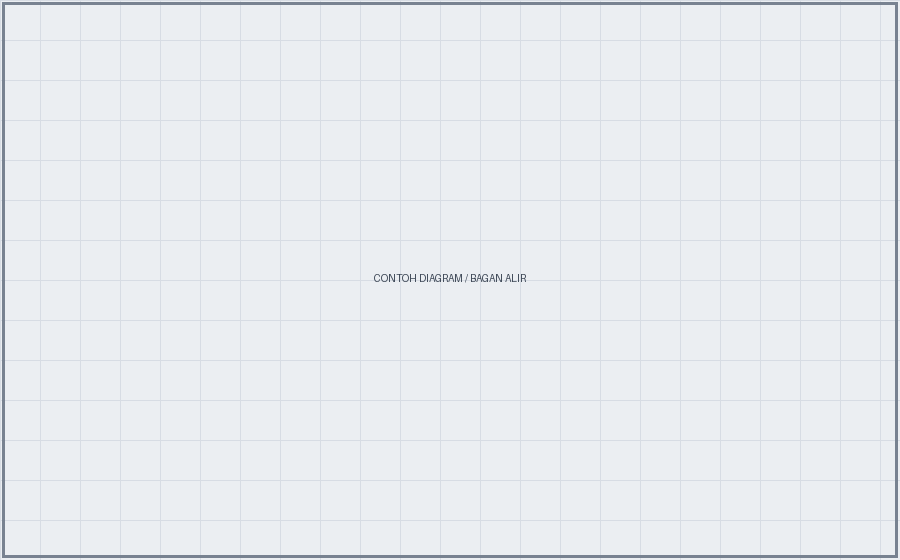
\includegraphics[width=0.75\linewidth]{contoh-diagram}
    \caption{Tahapan penelitian}
    \label{fig:tahapan}
\end{figure}

\begin{daftarnomor}
    \item \textbf{Studi pendahuluan.} Menelaah catatan layanan bantuan dan
          melakukan wawancara awal dengan pengelola sistem untuk memastikan
          masalah yang diteliti benar-benar terjadi.
    \item \textbf{Studi literatur.} Menelaah penelitian terdahulu dan landasan
          teori, serta menetapkan instrumen dan teknik analisis.
    \item \textbf{Penyusunan instrumen.} Menyiapkan kuesioner WebQual 4.0
          beserta terjemahan dan uji keterbacaannya.
    \item \textbf{Pengumpulan data.} Menyebarkan kuesioner kepada responden
          sesuai kriteria yang ditetapkan.
    \item \textbf{Pengujian instrumen.} Menguji validitas dan reliabilitas
          instrumen pada data yang terkumpul.
    \item \textbf{Analisis data.} Melakukan analisis deskriptif, analisis
          kesenjangan, dan pemetaan kuadran IPA.
    \item \textbf{Penarikan kesimpulan.} Menyusun kesimpulan yang menjawab
          setiap rumusan masalah.
\end{daftarnomor}

\section{Populasi dan Sampel}
Populasi penelitian adalah mahasiswa aktif yang telah menggunakan SIA minimal
dua semester, berjumlah 2.450 orang. Penentuan ukuran sampel menggunakan rumus
Slovin pada taraf kesalahan 10\% sebagaimana \cref{eq:slovin}.

\begin{equation}
    \label{eq:slovin}
    n = \frac{N}{1 + N e^{2}}
\end{equation}

\noindent dengan $n$ adalah ukuran sampel, $N$ adalah ukuran populasi, dan $e$
adalah taraf kesalahan. Berdasarkan perhitungan tersebut diperoleh ukuran
sampel minimum sebanyak 96 responden. Teknik pengambilan sampel yang digunakan
adalah \textit{purposive sampling} dengan kriteria inklusi berupa status
mahasiswa aktif dan pengalaman penggunaan minimal dua semester.

\section{Instrumen Penelitian}
Instrumen yang digunakan adalah WebQual 4.0 yang terdiri atas 22 butir pada tiga
dimensi. Setiap butir diukur pada dua skala Likert lima poin, yaitu tingkat
kepentingan dan tingkat kinerja. Instrumen digunakan tanpa penambahan maupun
pengurangan butir agar validitas aslinya tetap terjaga.

\section{Teknik Analisis Data}

\subsection{Pengujian Instrumen}
Validitas butir diuji menggunakan korelasi \textit{product moment}, dengan butir
dinyatakan valid apabila nilai $r_{hitung} > r_{tabel}$. Reliabilitas diuji
menggunakan koefisien \textit{Cronbach's alpha} sebagaimana \cref{eq:alpha},
dengan instrumen dinyatakan reliabel apabila nilainya di atas 0,70.

\begin{equation}
    \label{eq:alpha}
    \alpha = \frac{k}{k-1}\left(1 - \frac{\sum_{i=1}^{k} s_{i}^{2}}{s_{t}^{2}}\right)
\end{equation}

\noindent dengan $k$ adalah jumlah butir, $s_{i}^{2}$ adalah varians butir
ke-$i$, dan $s_{t}^{2}$ adalah varians skor total.

\subsection{Analisis Deskriptif}
Analisis deskriptif digunakan untuk menggambarkan tingkat kinerja setiap butir
dan setiap dimensi melalui nilai rata-rata dan simpangan baku.

\subsection{Analisis Kesenjangan}
Kesenjangan dihitung sebagai selisih antara rata-rata tingkat kinerja dan
rata-rata tingkat kepentingan pada setiap butir. Nilai negatif menunjukkan
kinerja yang belum memenuhi harapan pengguna.

\subsection{Importance-Performance Analysis}
Setiap butir dipetakan ke dalam diagram kartesius dengan sumbu mendatar berupa
tingkat kinerja dan sumbu tegak berupa tingkat kepentingan. Perpotongan sumbu
ditetapkan pada rata-rata keseluruhan, sehingga terbentuk empat kuadran:
prioritas utama, pertahankan prestasi, prioritas rendah, dan berlebihan.

\section{Matriks Keterkaitan Penelitian}

% MATRIKS INI ADALAH PENGAMAN PALING PENTING DALAM SELURUH NASKAH.
% Ia mencegah dua cacat yang paling sering terjadi:
%   (1) Bab 4 memuat pekerjaan yang tidak pernah ditanyakan di Bab 1;
%   (2) Bab 5 menjawab pertanyaan yang tidak pernah diajukan.
% Isi kolom terakhir HARUS menunjuk subbab yang benar-benar ada di Bab 4.

Keterkaitan antara rumusan masalah, tujuan, data, teknik analisis, dan penyajian
hasil disajikan pada \cref{tab:keterkaitan}. Matriks ini memastikan setiap
rumusan masalah benar-benar dijawab dan setiap hasil yang disajikan memang
ditanyakan.

\begin{table}[H]
    \centering
    \caption{Matriks keterkaitan penelitian}
    \label{tab:keterkaitan}
    \footnotesize
    \setlength{\tabcolsep}{4pt}
    \begin{tabular}{|c|p{2.9cm}|p{2.4cm}|p{3.3cm}|p{2.4cm}|}
        \hline
        \textbf{\labelrq} & \textbf{Tujuan} & \textbf{Data} &
        \textbf{Teknik analisis} & \textbf{Disajikan pada} \\ \hline

        \cref{rq:kualitas} & Mengukur tingkat kualitas layanan pada tiga dimensi &
        Skor kinerja 22 butir & Statistik deskriptif &
        Subbab \ref{sec:hasil-rq1} \\ \hline

        \cref{rq:kesenjangan} & Menganalisis kesenjangan kepentingan dan kinerja &
        Skor kepentingan dan kinerja & Analisis kesenjangan &
        Subbab \ref{sec:hasil-rq2} \\ \hline

        \cref{rq:prioritas} & Menentukan prioritas perbaikan &
        Hasil \cref{rq:kualitas,rq:kesenjangan} & \textit{Importance-\newline Performance Analysis} &
        Subbab \ref{sec:hasil-rq3} \\ \hline
    \end{tabular}
\end{table}

\section{Penggunaan Kecerdasan Buatan dalam Penelitian}
\label{sec:ai-penelitian}

Sesuai dengan prinsip transparansi dan integritas akademik, bagian ini
menjelaskan pemanfaatan teknologi kecerdasan buatan (\textit{Artificial
Intelligence}, AI) generatif dalam proses penelitian. Penggunaan AI dilakukan
secara terbatas, di bawah pengawasan penuh penulis, dan tidak menggantikan
penalaran, keahlian, maupun tanggung jawab penulis atas seluruh keputusan
penelitian.

\noindent\textbf{Catatan pemakaian templat:} isi subbab ini hanya bila AI benar-benar
digunakan pada proses \emph{penelitian} (mis. analisis data, penyusunan atau
pemeriksaan kode, perancangan struktur basis data). Bila AI hanya digunakan untuk
proses \emph{penulisan}, cukup gunakan halaman ``Pernyataan Penggunaan Kecerdasan
Buatan'' sebelum Daftar Pustaka. Bila AI tidak digunakan sama sekali, hapus subbab
ini beserta \texttt{\textbackslash include\{xx-deklarasi-ai\}} pada
\texttt{laporan.tex}.

Dalam penelitian ini, AI generatif (\belumdiisi{sebutkan nama dan versi alat,
mis. ChatGPT/GPT-4, Claude}) dimanfaatkan pada tahapan berikut:

\begin{daftarnomor}
    \item \textbf{Bantuan analisis atau pengolahan data.} \belumdiisi{jelaskan
          penggunaannya; seluruh perhitungan dan penafsiran diperiksa sendiri oleh
          penulis.}
    \item \textbf{Bantuan penyusunan atau pemeriksaan kode.} \belumdiisi{jelaskan
          penggunaannya; seluruh kode diverifikasi dan diuji sendiri oleh penulis.}
    \item \textbf{Bantuan perancangan struktur.} \belumdiisi{jelaskan
          penggunaannya; hasilnya divalidasi kesesuaiannya oleh penulis.}
\end{daftarnomor}

AI \textbf{tidak} digunakan untuk mengarang data, membuat hasil pengujian fiktif,
maupun menghasilkan sumber rujukan tanpa verifikasi. Seluruh keluaran AI telah
penulis periksa, sunting, dan validasi, sehingga penulis bertanggung jawab penuh
atas keakuratan dan integritas seluruh isi penelitian. Penggunaan AI untuk sekadar
pemeriksaan tata bahasa dan ejaan tidak termasuk yang dinyatakan di sini.

%==================================================================
% BAB 4 — HASIL DAN PEMBAHASAN
%
% STRUKTUR WAJIB: hasil disajikan PER RUMUSAN MASALAH, dengan urutan
% dan penomoran yang sama seperti pada matriks keterkaitan di Bab 3.
% Jangan menyajikan hasil yang tidak pernah ditanyakan.
%==================================================================

\chapter{HASIL DAN PEMBAHASAN}

\section{Gambaran Umum Responden}
Kuesioner disebarkan kepada mahasiswa aktif yang memenuhi kriteria inklusi dan
memperoleh 96 tanggapan yang lengkap. Sebaran responden berdasarkan angkatan
dan frekuensi penggunaan sistem disajikan pada \cref{tab:responden}.

\begin{table}[H]
    \centering
    \caption{Karakteristik responden}
    \label{tab:responden}
    \begin{tabular}{|l|c|c|}
        \hline
        \textbf{Karakteristik} & \textbf{Jumlah} & \textbf{Persentase} \\ \hline
        Angkatan 2022 & 31 & 32,3\% \\ \hline
        Angkatan 2023 & 34 & 35,4\% \\ \hline
        Angkatan 2024 & 31 & 32,3\% \\ \hline
        \textbf{Total} & \textbf{96} & \textbf{100\%} \\ \hline
    \end{tabular}
\end{table}

\section{Hasil Pengujian Instrumen}
Seluruh 22 butir dinyatakan valid karena nilai $r_{hitung}$ berada di atas
$r_{tabel}$ sebesar 0,201 pada taraf signifikansi 5\%. Nilai
\textit{Cronbach's alpha} sebesar 0,912 menunjukkan instrumen reliabel untuk
digunakan pada data penelitian ini.

% ==================================================================
% HASIL — disusun per rumusan masalah
% Perhatikan \label pada setiap subbab: label inilah yang dirujuk
% oleh matriks keterkaitan di Bab 3.
% ==================================================================

\section{Tingkat Kualitas Layanan}
\label{sec:hasil-rq1}
% Menjawab RQ1

Hasil pengukuran tingkat kinerja pada ketiga dimensi WebQual 4.0 disajikan pada
\cref{tab:dimensi}.

\begin{table}[H]
    \centering
    \caption{Tingkat kinerja per dimensi}
    \label{tab:dimensi}
    \begin{tabular}{|l|c|c|c|}
        \hline
        \textbf{Dimensi} & \textbf{Jumlah butir} & \textbf{Rata-rata} & \textbf{Kategori} \\ \hline
        \textit{Usability}                  & 8 & 3,12 & Cukup \\ \hline
        \textit{Information quality}        & 7 & 3,68 & Baik  \\ \hline
        \textit{Service interaction quality}& 7 & 3,54 & Baik  \\ \hline
    \end{tabular}
\end{table}

Berdasarkan \cref{tab:dimensi}, dimensi \textit{usability} memperoleh nilai
rata-rata terendah, yaitu 3,12, sedangkan \textit{information quality}
memperoleh nilai tertinggi sebesar 3,68.

\section{Kesenjangan Kepentingan dan Kinerja}
\label{sec:hasil-rq2}
% Menjawab RQ2

Perbandingan tingkat kepentingan dan tingkat kinerja pada setiap dimensi
disajikan pada \cref{tab:gap}.

\begin{table}[H]
    \centering
    \caption{Kesenjangan kepentingan dan kinerja per dimensi}
    \label{tab:gap}
    \begin{tabular}{|l|c|c|c|}
        \hline
        \textbf{Dimensi} & \textbf{Kepentingan} & \textbf{Kinerja} & \textbf{Kesenjangan} \\ \hline
        \textit{Usability}                  & 4,41 & 3,12 & $-1{,}29$ \\ \hline
        \textit{Information quality}        & 4,22 & 3,68 & $-0{,}54$ \\ \hline
        \textit{Service interaction quality}& 4,05 & 3,54 & $-0{,}51$ \\ \hline
    \end{tabular}
\end{table}

Seluruh dimensi memperoleh nilai kesenjangan negatif, yang menunjukkan kinerja
belum memenuhi harapan pengguna. Kesenjangan terbesar terjadi pada dimensi
\textit{usability}, khususnya pada butir kemudahan navigasi sebesar $-1{,}58$.

\section{Prioritas Perbaikan}
\label{sec:hasil-rq3}
% Menjawab RQ3

Pemetaan seluruh butir ke dalam diagram kartesius IPA ditunjukkan pada
\cref{fig:kuadran}.

\begin{figure}[H]
    \centering
    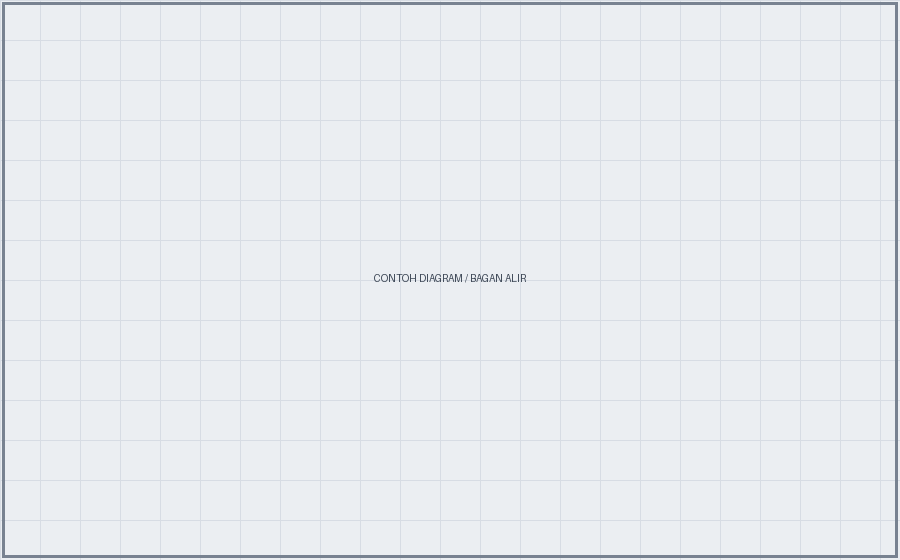
\includegraphics[width=0.7\linewidth]{contoh-diagram}
    \caption{Pemetaan kuadran \textit{Importance-Performance Analysis}}
    \label{fig:kuadran}
\end{figure}

Sebanyak lima butir berada pada kuadran prioritas utama, yaitu kuadran dengan
tingkat kepentingan tinggi namun tingkat kinerja rendah. Kelima butir tersebut
disajikan pada \cref{tab:prioritas}.

\begin{table}[H]
    \centering
    \caption{Butir pada kuadran prioritas utama}
    \label{tab:prioritas}
    \footnotesize
    \begin{tabular}{|c|p{7.5cm}|c|c|}
        \hline
        \textbf{No} & \textbf{Butir} & \textbf{Kepentingan} & \textbf{Kinerja} \\ \hline
        1 & Kemudahan menemukan menu yang dibutuhkan & 4,58 & 3,00 \\ \hline
        2 & Kejelasan alur pengisian rencana studi   & 4,52 & 3,05 \\ \hline
        3 & Kemudahan mempelajari cara pengoperasian & 4,44 & 3,10 \\ \hline
        4 & Kejelasan pesan kesalahan sistem         & 4,39 & 3,08 \\ \hline
        5 & Kemudahan navigasi antarhalaman          & 4,61 & 3,03 \\ \hline
    \end{tabular}
\end{table}

Kelima butir tersebut seluruhnya berasal dari dimensi \textit{usability} dan
berkaitan dengan navigasi serta kejelasan alur, bukan dengan ketersediaan
fitur.

% ==================================================================
% PEMBAHASAN — juga disusun per rumusan masalah
%
% POLA EMPAT LANGKAH untuk setiap subbab pembahasan:
%   (1) nyatakan ulang temuan secara ringkas;
%   (2) bandingkan dengan penelitian terdahulu YANG SAMA dengan yang
%       diperkenalkan pada latar belakang Bab 1;
%   (3) jelaskan mengapa sejalan atau mengapa berbeda;
%   (4) tarik implikasinya.
%
% Perhatikan bahwa pembahasan di bawah memuat KEDUANYA: temuan yang
% sejalan DAN temuan yang bertentangan dengan penelitian terdahulu.
% Temuan yang bertentangan bukan kelemahan, melainkan bahan analisis.
% ==================================================================

\section{Pembahasan}

\subsection{Pembahasan Tingkat Kualitas Layanan}
% Membahas hasil pada Subbab \ref{sec:hasil-rq1}

Hasil pada Subbab \ref{sec:hasil-rq1} menunjukkan dimensi \textit{usability}
memperoleh skor kinerja terendah di antara ketiga dimensi. Temuan ini sejalan
dengan hasil \citet{wijaya2022}, yang juga menemukan \textit{usability} sebagai
dimensi dengan penilaian terendah pada sistem informasi akademik, dengan
keluhan navigasi sebagai penyumbang utama.

Kesesuaian ini menguatkan dugaan bahwa persoalan utama sistem informasi
akademik terletak pada arsitektur informasi antarmuka, bukan pada kelengkapan
fitur maupun keakuratan data yang disajikan. Implikasinya, upaya perbaikan yang
menambah fitur baru berpotensi tidak menyelesaikan keluhan pengguna selama
persoalan navigasi belum dibenahi.

\subsection{Pembahasan Kesenjangan Kepentingan dan Kinerja}
% Membahas hasil pada Subbab \ref{sec:hasil-rq2}

Hasil pada Subbab \ref{sec:hasil-rq2} menunjukkan seluruh dimensi memiliki
kesenjangan negatif, dengan kesenjangan terbesar pada \textit{usability}.
Temuan ini berbeda dengan \citet{pratama2023} yang melaporkan
\textit{service interaction quality} sebagai dimensi paling berpengaruh
terhadap kepuasan pengguna.

Perbedaan tersebut dapat dijelaskan melalui karakteristik pengguna. Responden
pada penelitian \citet{pratama2023} merupakan pengguna insidental layanan
pemerintah daerah yang berinteraksi langsung dengan petugas, sehingga aspek
interaksi layanan menjadi menonjol. Sebaliknya, responden pada penelitian ini
menggunakan sistem secara mandiri tanpa pendampingan petugas, sehingga
kemudahan penggunaan antarmuka menjadi aspek yang paling dirasakan. Penjelasan
ini konsisten dengan \citet{sari2024} yang menyatakan hasil pengukuran kualitas
layanan sangat dipengaruhi karakteristik pengguna dan pola penggunaannya.

\subsection{Pembahasan Prioritas Perbaikan}
% Membahas hasil pada Subbab \ref{sec:hasil-rq3}

Hasil pada Subbab \ref{sec:hasil-rq3} menempatkan lima butir pada kuadran
prioritas utama, seluruhnya berkaitan dengan navigasi dan kejelasan alur.
Penelitian terdahulu yang menggunakan WebQual 4.0 umumnya berhenti pada
penyajian skor per dimensi \citep{wijaya2022, pratama2023}, sehingga belum
menghasilkan urutan prioritas pada tingkat butir.

Pemetaan kuadran pada penelitian ini menunjukkan bahwa meskipun dimensi
\textit{information quality} memperoleh skor tertinggi, terdapat butir di
dalamnya yang tetap masuk kuadran prioritas rendah karena tingkat
kepentingannya juga rendah. Temuan ini menegaskan bahwa keputusan perbaikan
tidak dapat didasarkan pada skor dimensi semata, melainkan perlu
mempertimbangkan tingkat kepentingan tiap butir menurut pengguna.

%==================================================================
% BAB 5 — KESIMPULAN DAN SARAN
%
% Kesimpulan disusun BERNOMOR SEJAJAR dengan rumusan masalah:
% butir 1 menjawab RQ1, butir 2 menjawab RQ2, butir 3 menjawab RQ3.
% Jangan menambahkan butir kesimpulan yang tidak menjawab rumusan
% masalah mana pun, dan jangan meninggalkan rumusan masalah tanpa
% kesimpulan.
%==================================================================

\chapter{KESIMPULAN DAN SARAN}

\section{Kesimpulan}
Berdasarkan hasil penelitian dan pembahasan, diperoleh kesimpulan berikut.

\begin{daftarnomor}
    \item Kualitas layanan SIA berada pada kategori cukup hingga baik, dengan
          dimensi \textit{usability} memperoleh nilai kinerja terendah sebesar
          3,12 dan \textit{information quality} tertinggi sebesar 3,68.
          \emph{(menjawab \cref{rq:kualitas})}
    \item Seluruh dimensi memiliki kesenjangan negatif antara kepentingan dan
          kinerja. Kesenjangan terbesar terjadi pada dimensi \textit{usability}
          sebesar $-1{,}29$, dengan butir kemudahan navigasi sebagai
          penyumbang terbesar. \emph{(menjawab \cref{rq:kesenjangan})}
    \item Terdapat lima butir yang berada pada kuadran prioritas utama dan
          seluruhnya berkaitan dengan navigasi serta kejelasan alur, sehingga
          perbaikan disarankan diarahkan pada arsitektur informasi antarmuka.
          \emph{(menjawab \cref{rq:prioritas})}
\end{daftarnomor}

\section{Keterbatasan Penelitian}
% Subbab ini opsional pada sebagian program studi, namun sangat
% disarankan. Menyatakan keterbatasan secara jujur memperkuat
% kredibilitas, dan mendahului pertanyaan penguji.

\begin{daftarnomor}
    \item Penelitian dilakukan pada satu perguruan tinggi, sehingga hasilnya
          belum dapat digeneralisasi ke sistem informasi akademik lain.
    \item Pengukuran bersifat persepsional dan belum dilengkapi pengujian
          teknis terhadap antarmuka maupun kinerja sistem.
\end{daftarnomor}

\section{Saran}

\begin{daftarnomor}
    \item Bagi pengelola sistem, perbaikan disarankan dimulai dari kelima butir
          pada kuadran prioritas utama, khususnya penataan ulang struktur menu
          dan penyederhanaan alur pengisian rencana studi.
    \item Bagi penelitian selanjutnya, hasil pengukuran persepsional ini dapat
          dilengkapi dengan pengujian ketergunaan berbasis tugas untuk
          memperoleh bukti perilaku, bukan hanya persepsi.
    \item Penelitian serupa dapat dilakukan pada beberapa perguruan tinggi
          sekaligus agar diperoleh gambaran yang lebih dapat digeneralisasi.
\end{daftarnomor}


%------------------ BAGIAN AKHIR ----------------------------------
%==================================================================
% PERNYATAAN PENGGUNAAN KECERDASAN BUATAN DALAM PENULISAN
%
% Mengikuti kelaziman jurnal internasional (mis. Elsevier), pernyataan
% penggunaan AI pada proses PENULISAN diletakkan pada bagian tersendiri
% tepat SEBELUM Daftar Pustaka. Sebutkan nama alat, tujuan penggunaan,
% dan pernyataan tanggung jawab penulis.
%
% Penggunaan AI dalam proses PENELITIAN dijelaskan terpisah pada Bab 3
% (lihat \cref{sec:ai-penelitian}).
%
% Bila AI tidak dipakai untuk penulisan, beri tanda % pada baris
% %==================================================================
% PERNYATAAN PENGGUNAAN KECERDASAN BUATAN DALAM PENULISAN
%
% Mengikuti kelaziman jurnal internasional (mis. Elsevier), pernyataan
% penggunaan AI pada proses PENULISAN diletakkan pada bagian tersendiri
% tepat SEBELUM Daftar Pustaka. Sebutkan nama alat, tujuan penggunaan,
% dan pernyataan tanggung jawab penulis.
%
% Penggunaan AI dalam proses PENELITIAN dijelaskan terpisah pada Bab 3
% (lihat \cref{sec:ai-penelitian}).
%
% Bila AI tidak dipakai untuk penulisan, beri tanda % pada baris
% %==================================================================
% PERNYATAAN PENGGUNAAN KECERDASAN BUATAN DALAM PENULISAN
%
% Mengikuti kelaziman jurnal internasional (mis. Elsevier), pernyataan
% penggunaan AI pada proses PENULISAN diletakkan pada bagian tersendiri
% tepat SEBELUM Daftar Pustaka. Sebutkan nama alat, tujuan penggunaan,
% dan pernyataan tanggung jawab penulis.
%
% Penggunaan AI dalam proses PENELITIAN dijelaskan terpisah pada Bab 3
% (lihat \cref{sec:ai-penelitian}).
%
% Bila AI tidak dipakai untuk penulisan, beri tanda % pada baris
% \include{xx-deklarasi-ai} di laporan.tex.
%==================================================================
\clearpage
\phantomsection
\addcontentsline{toc}{chapter}{PERNYATAAN PENGGUNAAN KECERDASAN BUATAN}
\begin{center}
    \textbf{\large PERNYATAAN PENGGUNAAN KECERDASAN BUATAN}\\
    \textbf{\large DALAM PROSES PENULISAN}\\[2em]
\end{center}

Selama proses penyusunan naskah Tugas Akhir ini, penulis menggunakan
\belumdiisi{sebutkan nama dan versi alat AI, mis. ChatGPT (GPT-4), Claude, atau
Grammarly} untuk \belumdiisi{sebutkan tujuannya, mis. membantu merapikan dan
memperbaiki keterbacaan bahasa, menata struktur penulisan, serta menerjemahkan
abstrak ke dalam Bahasa Inggris}. Setelah menggunakan alat tersebut, penulis
telah meninjau dan menyunting seluruh isinya sesuai kebutuhan dan bertanggung
jawab penuh atas isi naskah Tugas Akhir ini.

\vspace{0.8em}
\noindent Pernyataan ini tidak berlaku untuk penggunaan alat bantu dasar seperti
pemeriksa tata bahasa, ejaan, dan tanda baca. Kecerdasan buatan tidak dicantumkan
sebagai penulis maupun sebagai sumber rujukan dalam Tugas Akhir ini.

\vspace{2em}
\begin{flushright}
    \kota, \tglpernyataan\\[0.8em]
    Penulis,\\[2cm]
    \penulis\\
    NIM. \nim
\end{flushright}
\clearpage
 di laporan.tex.
%==================================================================
\clearpage
\phantomsection
\addcontentsline{toc}{chapter}{PERNYATAAN PENGGUNAAN KECERDASAN BUATAN}
\begin{center}
    \textbf{\large PERNYATAAN PENGGUNAAN KECERDASAN BUATAN}\\
    \textbf{\large DALAM PROSES PENULISAN}\\[2em]
\end{center}

Selama proses penyusunan naskah Tugas Akhir ini, penulis menggunakan
\belumdiisi{sebutkan nama dan versi alat AI, mis. ChatGPT (GPT-4), Claude, atau
Grammarly} untuk \belumdiisi{sebutkan tujuannya, mis. membantu merapikan dan
memperbaiki keterbacaan bahasa, menata struktur penulisan, serta menerjemahkan
abstrak ke dalam Bahasa Inggris}. Setelah menggunakan alat tersebut, penulis
telah meninjau dan menyunting seluruh isinya sesuai kebutuhan dan bertanggung
jawab penuh atas isi naskah Tugas Akhir ini.

\vspace{0.8em}
\noindent Pernyataan ini tidak berlaku untuk penggunaan alat bantu dasar seperti
pemeriksa tata bahasa, ejaan, dan tanda baca. Kecerdasan buatan tidak dicantumkan
sebagai penulis maupun sebagai sumber rujukan dalam Tugas Akhir ini.

\vspace{2em}
\begin{flushright}
    \kota, \tglpernyataan\\[0.8em]
    Penulis,\\[2cm]
    \penulis\\
    NIM. \nim
\end{flushright}
\clearpage
 di laporan.tex.
%==================================================================
\clearpage
\phantomsection
\addcontentsline{toc}{chapter}{PERNYATAAN PENGGUNAAN KECERDASAN BUATAN}
\begin{center}
    \textbf{\large PERNYATAAN PENGGUNAAN KECERDASAN BUATAN}\\
    \textbf{\large DALAM PROSES PENULISAN}\\[2em]
\end{center}

Selama proses penyusunan naskah Tugas Akhir ini, penulis menggunakan
\belumdiisi{sebutkan nama dan versi alat AI, mis. ChatGPT (GPT-4), Claude, atau
Grammarly} untuk \belumdiisi{sebutkan tujuannya, mis. membantu merapikan dan
memperbaiki keterbacaan bahasa, menata struktur penulisan, serta menerjemahkan
abstrak ke dalam Bahasa Inggris}. Setelah menggunakan alat tersebut, penulis
telah meninjau dan menyunting seluruh isinya sesuai kebutuhan dan bertanggung
jawab penuh atas isi naskah Tugas Akhir ini.

\vspace{0.8em}
\noindent Pernyataan ini tidak berlaku untuk penggunaan alat bantu dasar seperti
pemeriksa tata bahasa, ejaan, dan tanda baca. Kecerdasan buatan tidak dicantumkan
sebagai penulis maupun sebagai sumber rujukan dalam Tugas Akhir ini.

\vspace{2em}
\begin{flushright}
    \kota, \tglpernyataan\\[0.8em]
    Penulis,\\[2cm]
    \penulis\\
    NIM. \nim
\end{flushright}
\clearpage

%==================================================================
% DAFTAR PUSTAKA  (dihasilkan otomatis dari a7-pustaka.bib)
%
% Hanya rujukan yang benar-benar disitasi di dalam naskah yang akan
% muncul di sini. Jika ingin menampilkan SELURUH entri pada berkas
% .bib meskipun tidak disitasi, aktifkan baris \nocite{*} di bawah.
%==================================================================
\clearpage
\phantomsection
\addcontentsline{toc}{chapter}{\bibname}
\begin{center}
    \textbf{\large \bibname}\\[1.5em]
\end{center}

% \nocite{*}
\bibliography{a7-pustaka}

%==================================================================
% LAMPIRAN
%
% Setiap lampiran didaftarkan ke DAFTAR LAMPIRAN dengan perintah
% \daftarlampiran{...}
%
% Penomoran gambar dan tabel di dalam lampiran otomatis berubah
% menjadi A.1, A.2, B.1, dan seterusnya.
%==================================================================
\clearpage
\appendix
\renewcommand{\thefigure}{\Alph{chapter}.\arabic{figure}}
\renewcommand{\thetable}{\Alph{chapter}.\arabic{table}}

%------------------------------------------------------------------
\chapter{INSTRUMEN PENELITIAN}
\daftarlampiran{Lampiran A \quad Instrumen Penelitian}

Lampirkan instrumen lengkap yang digunakan, misalnya kuesioner, pedoman
wawancara, atau lembar validasi pakar.

\begin{table}[H]
    \centering
    \caption{Contoh butir instrumen}
    \begin{tabular}{|c|p{8cm}|c|}
        \hline
        \textbf{No} & \textbf{Pernyataan} & \textbf{Dimensi} \\ \hline
        1 & Saya merasa sistem mudah dipelajari.       & \textit{Usability} \\ \hline
        2 & Informasi yang disajikan sistem akurat.    & \textit{Information quality} \\ \hline
        3 & Sistem memberikan tanggapan yang memadai.  & \textit{Service interaction} \\ \hline
    \end{tabular}
\end{table}

%------------------------------------------------------------------
\chapter{DATA HASIL PENELITIAN}
\daftarlampiran{Lampiran B \quad Data Hasil Penelitian}

Lampirkan rekapitulasi data mentah, hasil perhitungan, atau keluaran perangkat
lunak analisis.

\begin{figure}[H]
    \centering
    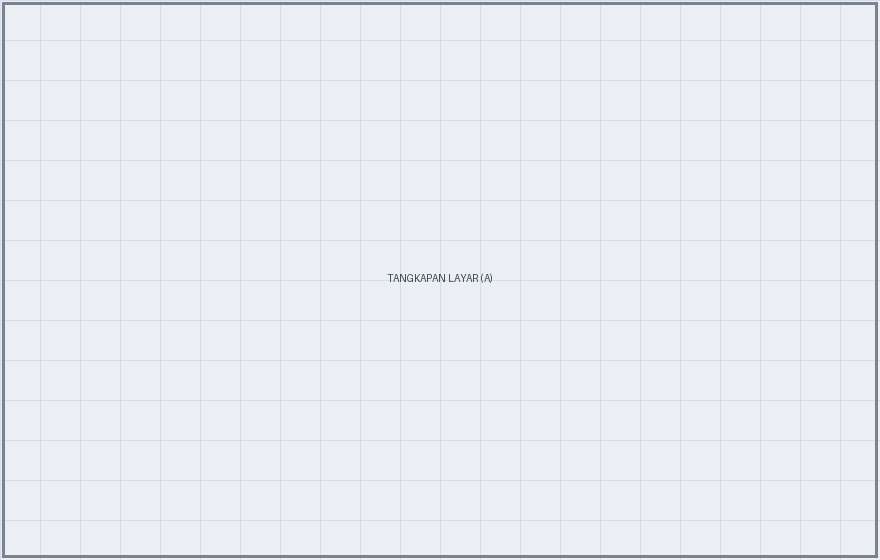
\includegraphics[width=0.8\linewidth]{contoh-tangkapan-a}
    \caption{Contoh rekapitulasi data}
\end{figure}

%------------------------------------------------------------------
\chapter{DOKUMENTASI}
\daftarlampiran{Lampiran C \quad Dokumentasi}

Lampirkan dokumentasi kegiatan penelitian, surat izin, atau berita acara
pengujian.


%==================================================================
% GALERI ELEMEN — contoh tabel, gambar, rumus, kode, dan sitasi.
% HAPUS ATAU BERI TANDA % PADA BARIS DI BAWAH sebelum naskah dikumpulkan.
%==================================================================
%%==================================================================
% GALERI ELEMEN
%
% Berkas ini berisi CONTOH SIAP SALIN untuk seluruh elemen yang lazim
% dibutuhkan pada Tugas Akhir: berbagai jenis tabel, gambar, rumus,
% kode program, pseudocode, dan pola sitasi.
%
% CARA MEMATIKANNYA
% Beri tanda % pada baris %==================================================================
% GALERI ELEMEN
%
% Berkas ini berisi CONTOH SIAP SALIN untuk seluruh elemen yang lazim
% dibutuhkan pada Tugas Akhir: berbagai jenis tabel, gambar, rumus,
% kode program, pseudocode, dan pola sitasi.
%
% CARA MEMATIKANNYA
% Beri tanda % pada baris %==================================================================
% GALERI ELEMEN
%
% Berkas ini berisi CONTOH SIAP SALIN untuk seluruh elemen yang lazim
% dibutuhkan pada Tugas Akhir: berbagai jenis tabel, gambar, rumus,
% kode program, pseudocode, dan pola sitasi.
%
% CARA MEMATIKANNYA
% Beri tanda % pada baris \include{zz-galeri-elemen} di laporan.tex
% sebelum naskah dikumpulkan. Berkas ini tidak akan ikut tercetak,
% tetapi tetap tersimpan sebagai rujukan.
%==================================================================

% Galeri disertakan setelah lampiran, sehingga tanpa pengaturan ini
% penomorannya akan ikut melanjutkan huruf lampiran (D, E, dst.).
% Blok berikut membuatnya bernomor "G" agar jelas terpisah.
\clearpage
\setcounter{chapter}{0}
\setcounter{figure}{0}
\setcounter{table}{0}
\setcounter{equation}{0}
\renewcommand{\thechapter}{G}
\renewcommand{\thesection}{G.\arabic{section}}
\renewcommand{\thesubsection}{\thesection.\arabic{subsection}}
\renewcommand{\thefigure}{G.\arabic{figure}}
\renewcommand{\thetable}{G.\arabic{table}}
\renewcommand{\theequation}{G.\arabic{equation}}

\chapter*{GALERI ELEMEN (HAPUS SEBELUM DIKUMPULKAN)}
\addcontentsline{toc}{chapter}{GALERI ELEMEN (HAPUS SEBELUM DIKUMPULKAN)}

Bab ini bukan bagian dari naskah Tugas Akhir. Isinya adalah contoh siap salin
untuk seluruh elemen yang lazim dibutuhkan. Matikan dengan memberi tanda
\texttt{\%} pada baris \texttt{\textbackslash include\{zz-galeri-elemen\}} di
berkas \texttt{laporan.tex}.

% ==================================================================
\section{Tabel}
% ==================================================================

\subsection{Tabel biasa}
Keterangan tabel diletakkan di \textbf{atas} tabel. Setiap tabel wajib diberi
\texttt{\textbackslash label} dan disebut dalam teks, misalnya
\cref{tab:g-biasa}.

\begin{table}[H]
    \centering
    \caption{Contoh tabel biasa}
    \label{tab:g-biasa}
    \begin{tabular}{|c|l|c|}
        \hline
        \textbf{No} & \textbf{Keterangan} & \textbf{Nilai} \\ \hline
        1 & Baris pertama & 3,12 \\ \hline
        2 & Baris kedua   & 3,68 \\ \hline
        3 & Baris ketiga  & 3,54 \\ \hline
    \end{tabular}
\end{table}

\subsection{Tabel dengan garis gaya ilmiah (booktabs)}
Sebagian program studi menghendaki tabel tanpa garis vertikal.

\begin{table}[H]
    \centering
    \caption{Contoh tabel gaya booktabs}
    \label{tab:g-booktabs}
    \begin{tabular}{lcc}
        \toprule
        \textbf{Dimensi} & \textbf{Kepentingan} & \textbf{Kinerja} \\
        \midrule
        \textit{Usability}           & 4,41 & 3,12 \\
        \textit{Information quality} & 4,22 & 3,68 \\
        \bottomrule
    \end{tabular}
\end{table}

\subsection{Tabel bersambung antarhalaman (longtable)}
Gunakan \texttt{longtable} bila tabel lebih panjang daripada satu halaman.
Baris kepala akan diulang otomatis, dan halaman sambungan diberi keterangan
``Lanjutan'' sesuai kelaziman naskah Indonesia.

\begin{longtable}{|c|p{6.5cm}|c|c|}
    \caption{Contoh tabel bersambung antarhalaman}
    \label{tab:g-longtable} \\
    \hline
    \textbf{No} & \textbf{Pernyataan} & \textbf{Kepentingan} & \textbf{Kinerja} \\ \hline
    \endfirsthead

    \multicolumn{4}{l}{\footnotesize\textit{Lanjutan \cref{tab:g-longtable}}} \\
    \hline
    \textbf{No} & \textbf{Pernyataan} & \textbf{Kepentingan} & \textbf{Kinerja} \\ \hline
    \endhead

    \hline
    \multicolumn{4}{r}{\footnotesize\textit{Bersambung ke halaman berikutnya}} \\
    \endfoot

    \hline
    \endlastfoot

    1  & Saya merasa sistem mudah dipelajari & 4,44 & 3,10 \\ \hline
    2  & Interaksi dengan sistem jelas dan mudah dipahami & 4,38 & 3,21 \\ \hline
    3  & Sistem mudah dioperasikan & 4,41 & 3,15 \\ \hline
    4  & Navigasi antarhalaman terasa mudah & 4,61 & 3,03 \\ \hline
    5  & Tampilan sistem sesuai dengan jenis layanannya & 4,02 & 3,44 \\ \hline
    6  & Tampilan sistem menarik & 3,88 & 3,52 \\ \hline
    7  & Sistem menyampaikan kesan kompeten & 4,12 & 3,40 \\ \hline
    8  & Sistem menciptakan pengalaman yang menyenangkan & 3,95 & 3,33 \\ \hline
    9  & Informasi yang disajikan akurat & 4,30 & 3,71 \\ \hline
    10 & Informasi yang disajikan tepercaya & 4,28 & 3,69 \\ \hline
    11 & Informasi selalu diperbarui & 4,19 & 3,58 \\ \hline
    12 & Informasi relevan dengan kebutuhan & 4,25 & 3,66 \\ \hline
    13 & Informasi mudah dipahami & 4,21 & 3,74 \\ \hline
    14 & Informasi disajikan pada tingkat rincian yang tepat & 4,08 & 3,70 \\ \hline
    15 & Informasi disajikan dalam format yang sesuai & 4,15 & 3,68 \\ \hline
    16 & Sistem memberikan rasa aman & 4,09 & 3,61 \\ \hline
    17 & Data pribadi terasa terlindungi & 4,18 & 3,55 \\ \hline
    18 & Sistem memudahkan komunikasi dengan pengelola & 3,97 & 3,42 \\ \hline
    19 & Sistem menciptakan rasa keterhubungan & 3,82 & 3,39 \\ \hline
    20 & Layanan diberikan sesuai yang dijanjikan & 4,11 & 3,58 \\ \hline
\end{longtable}

\subsection{Tabel dengan sel gabung (multirow dan multicolumn)}

\begin{table}[H]
    \centering
    \caption{Contoh tabel dengan sel gabung}
    \label{tab:g-gabung}
    \begin{tabular}{|c|c|c|c|c|}
        \hline
        \multirow{2}{*}{\textbf{Butir}} & \multicolumn{2}{c|}{\textbf{Sebelum}} & \multicolumn{2}{c|}{\textbf{Sesudah}} \\ \cline{2-5}
         & \textbf{Rerata} & \textbf{SB} & \textbf{Rerata} & \textbf{SB} \\ \hline
        B1 & 3,10 & 0,82 & 4,05 & 0,61 \\ \hline
        B2 & 3,22 & 0,77 & 4,12 & 0,58 \\ \hline
    \end{tabular}
\end{table}

\subsection{Tabel berkolom otomatis (tabularx)}
Lebar kolom bertipe \texttt{X} menyesuaikan sendiri agar tabel tepat memenuhi
lebar teks.

\begin{table}[H]
    \centering
    \caption{Contoh tabel dengan lebar kolom otomatis}
    \label{tab:g-tabularx}
    \begin{tabularx}{\textwidth}{|c|X|X|}
        \hline
        \textbf{No} & \textbf{Temuan} & \textbf{Tindak lanjut} \\ \hline
        1 & Menu utama tidak konsisten antarhalaman sehingga pengguna kehilangan orientasi. & Menyeragamkan struktur menu pada seluruh halaman. \\ \hline
        2 & Pesan kesalahan tidak menjelaskan penyebab masalah. & Menulis ulang pesan kesalahan dengan bahasa yang spesifik. \\ \hline
    \end{tabularx}
\end{table}

\subsection{Tabel dengan catatan kaki (threeparttable)}
Gunakan bila tabel memerlukan keterangan simbol atau sumber.

\begin{table}[H]
    \centering
    \begin{threeparttable}
        \caption{Contoh tabel dengan catatan kaki}
        \label{tab:g-catatan}
        \begin{tabular}{|l|c|c|}
            \hline
            \textbf{Dimensi} & \textbf{Rerata} & \textbf{Kategori} \\ \hline
            \textit{Usability}\tnote{a}           & 3,12 & Cukup \\ \hline
            \textit{Information quality}          & 3,68 & Baik  \\ \hline
            \textit{Service interaction}\tnote{b} & 3,54 & Baik  \\ \hline
        \end{tabular}
        \begin{tablenotes}\footnotesize
            \item[a] Terdiri atas 8 butir pernyataan.
            \item[b] Terdiri atas 7 butir pernyataan.
            \item Sumber: Hasil pengolahan data penelitian (2026).
        \end{tablenotes}
    \end{threeparttable}
\end{table}

\subsection{Tabel yang terlalu lebar}
Bila tabel sedikit melebihi lebar teks, perkecil jarak antarkolom dengan
\texttt{\textbackslash tabcolsep} atau bungkus dengan \texttt{adjustbox}.

\begin{table}[H]
    \centering
    \caption{Contoh tabel lebar yang dikecilkan otomatis}
    \label{tab:g-lebar}
    \footnotesize
    \begin{adjustbox}{max width=\textwidth}
    \begin{tabular}{|c|c|c|c|c|c|c|c|c|c|c|}
        \hline
        \textbf{Butir} & \textbf{R1} & \textbf{R2} & \textbf{R3} & \textbf{R4} & \textbf{R5} & \textbf{R6} & \textbf{R7} & \textbf{R8} & \textbf{Rerata} & \textbf{Simpangan Baku} \\ \hline
        B1 & 4 & 5 & 4 & 3 & 4 & 5 & 4 & 4 & 4,13 & 0,64 \\ \hline
        B2 & 3 & 4 & 4 & 4 & 5 & 4 & 3 & 4 & 3,88 & 0,64 \\ \hline
    \end{tabular}
    \end{adjustbox}
\end{table}

\subsection{Tabel lanskap}
Paket \texttt{pdflscape} ikut memutar halaman pada berkas PDF, sehingga pembaca
tidak perlu memiringkan kepala.

\begin{landscape}
\begin{table}[H]
    \centering
    \caption{Contoh tabel pada halaman lanskap}
    \label{tab:g-lanskap}
    \footnotesize
    \begin{tabular}{|c|p{4cm}|p{4cm}|p{4cm}|p{4cm}|}
        \hline
        \textbf{No} & \textbf{Kondisi berjalan} & \textbf{Masalah} & \textbf{Usulan} & \textbf{Dampak yang diharapkan} \\ \hline
        1 & Menu tersebar pada tiga tingkat & Pengguna kesulitan menemukan menu & Menyusun ulang menjadi dua tingkat & Waktu pencarian menu berkurang \\ \hline
        2 & Alur pengisian tidak menampilkan tahapan & Pengguna tidak tahu posisinya & Menambahkan penanda tahapan & Kesalahan pengisian berkurang \\ \hline
    \end{tabular}
\end{table}
\end{landscape}

% ==================================================================
\section{Gambar}
% ==================================================================

\subsection{Gambar tunggal}
Keterangan gambar diletakkan di \textbf{bawah} gambar. Lihat
\cref{fig:g-tunggal}.

\begin{figure}[H]
    \centering
    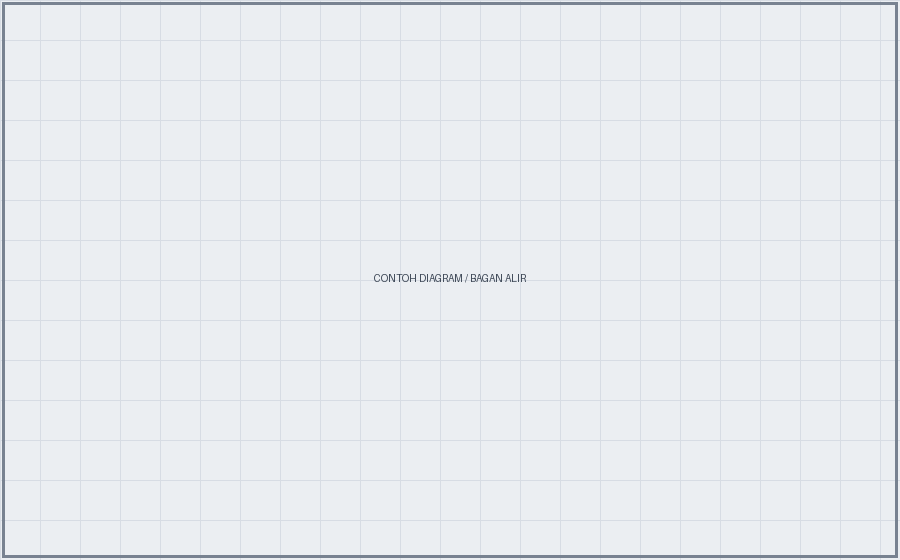
\includegraphics[width=0.6\linewidth]{contoh-diagram}
    \caption{Contoh gambar tunggal}
    \label{fig:g-tunggal}
\end{figure}

\subsection{Gambar dengan keterangan sumber}
Gunakan perintah \texttt{\textbackslash sumber} bila gambar dikutip dari
sumber lain.

\begin{figure}[H]
    \centering
    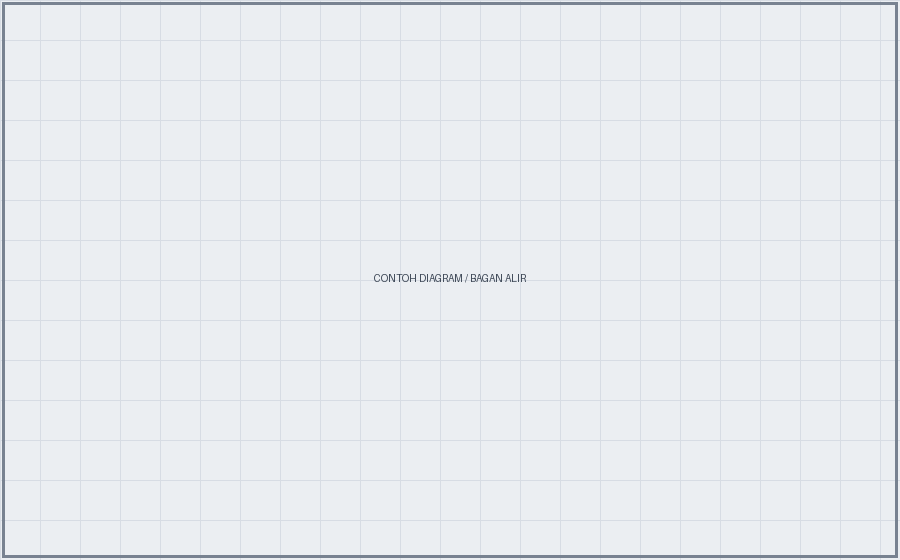
\includegraphics[width=0.55\linewidth]{contoh-diagram}
    \caption{Contoh gambar yang dikutip dari sumber lain}
    \label{fig:g-sumber}
\end{figure}
\sumber{\citet{barnes2002}}

\subsection{Dua gambar berdampingan}
Gunakan \texttt{subcaption} agar tiap bagian memperoleh label (a) dan (b) yang
dapat dirujuk terpisah, misalnya \cref{fig:g-kiri} dan \cref{fig:g-kanan}.

\begin{figure}[H]
    \centering
    \begin{subfigure}[t]{0.47\linewidth}
        \centering
        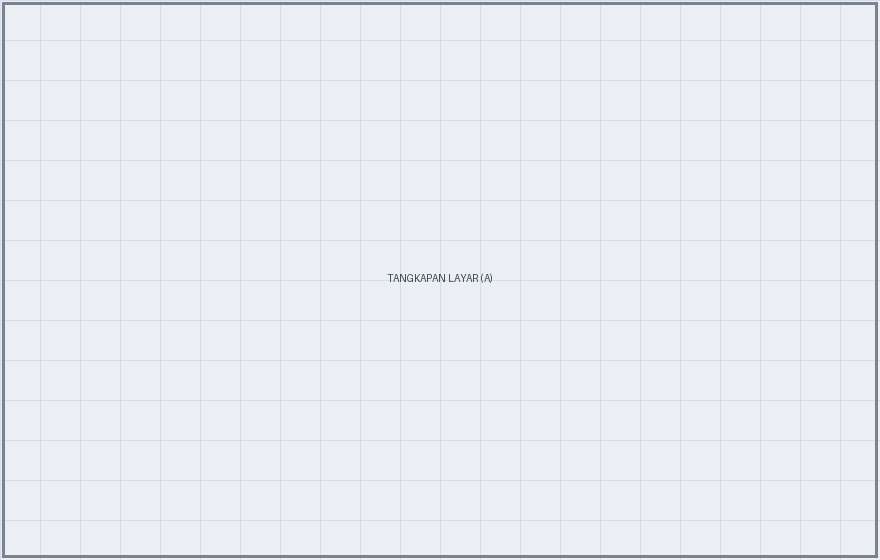
\includegraphics[width=\linewidth]{contoh-tangkapan-a}
        \caption{Tampilan sebelum perbaikan}
        \label{fig:g-kiri}
    \end{subfigure}
    \hfill
    \begin{subfigure}[t]{0.47\linewidth}
        \centering
        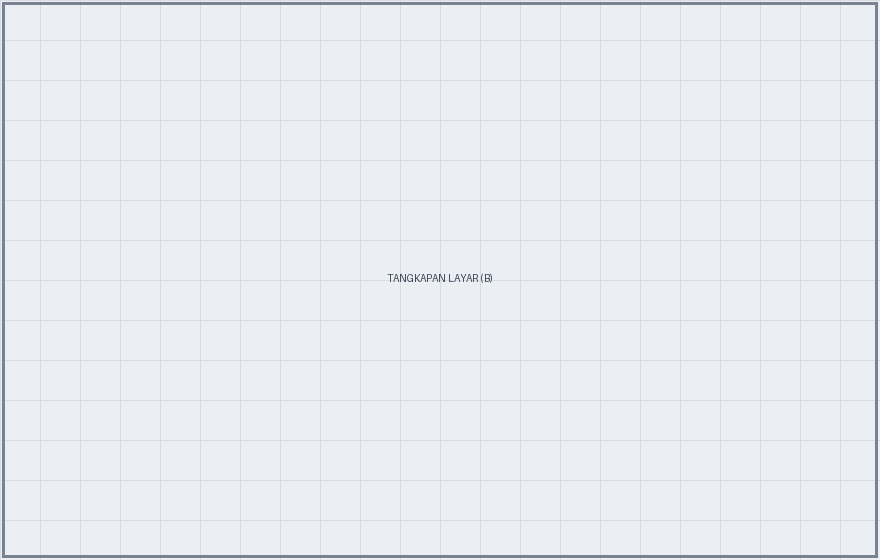
\includegraphics[width=\linewidth]{contoh-tangkapan-b}
        \caption{Tampilan sesudah perbaikan}
        \label{fig:g-kanan}
    \end{subfigure}
    \caption{Perbandingan tampilan antarmuka}
    \label{fig:g-berdampingan}
\end{figure}

\subsection{Gambar tinggi satu halaman}
Untuk gambar yang tinggi, seperti diagram alir panjang, gunakan
\texttt{height} agar tidak meluber ke halaman berikutnya.

\begin{figure}[H]
    \centering
    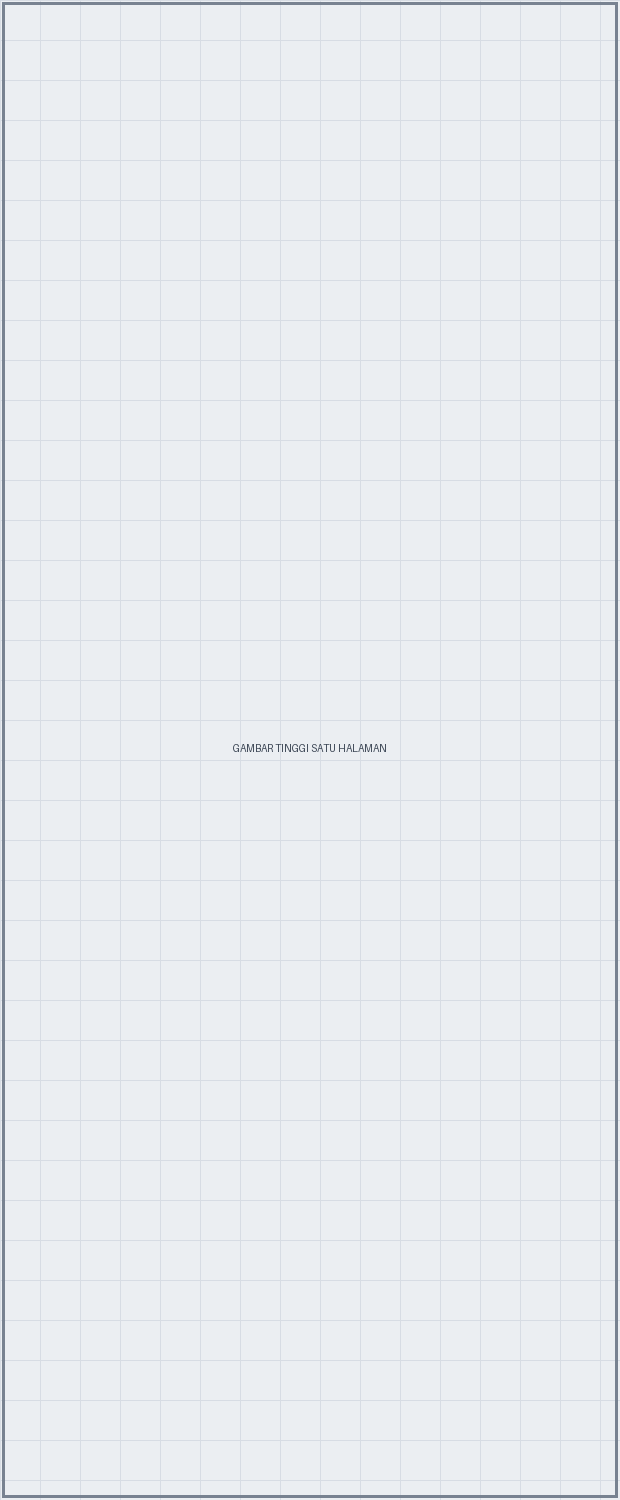
\includegraphics[height=0.78\textheight,keepaspectratio]{contoh-tinggi}
    \caption{Contoh gambar tinggi satu halaman}
    \label{fig:g-tinggi}
\end{figure}

\subsection{Gambar lanskap}

\begin{landscape}
\begin{figure}[H]
    \centering
    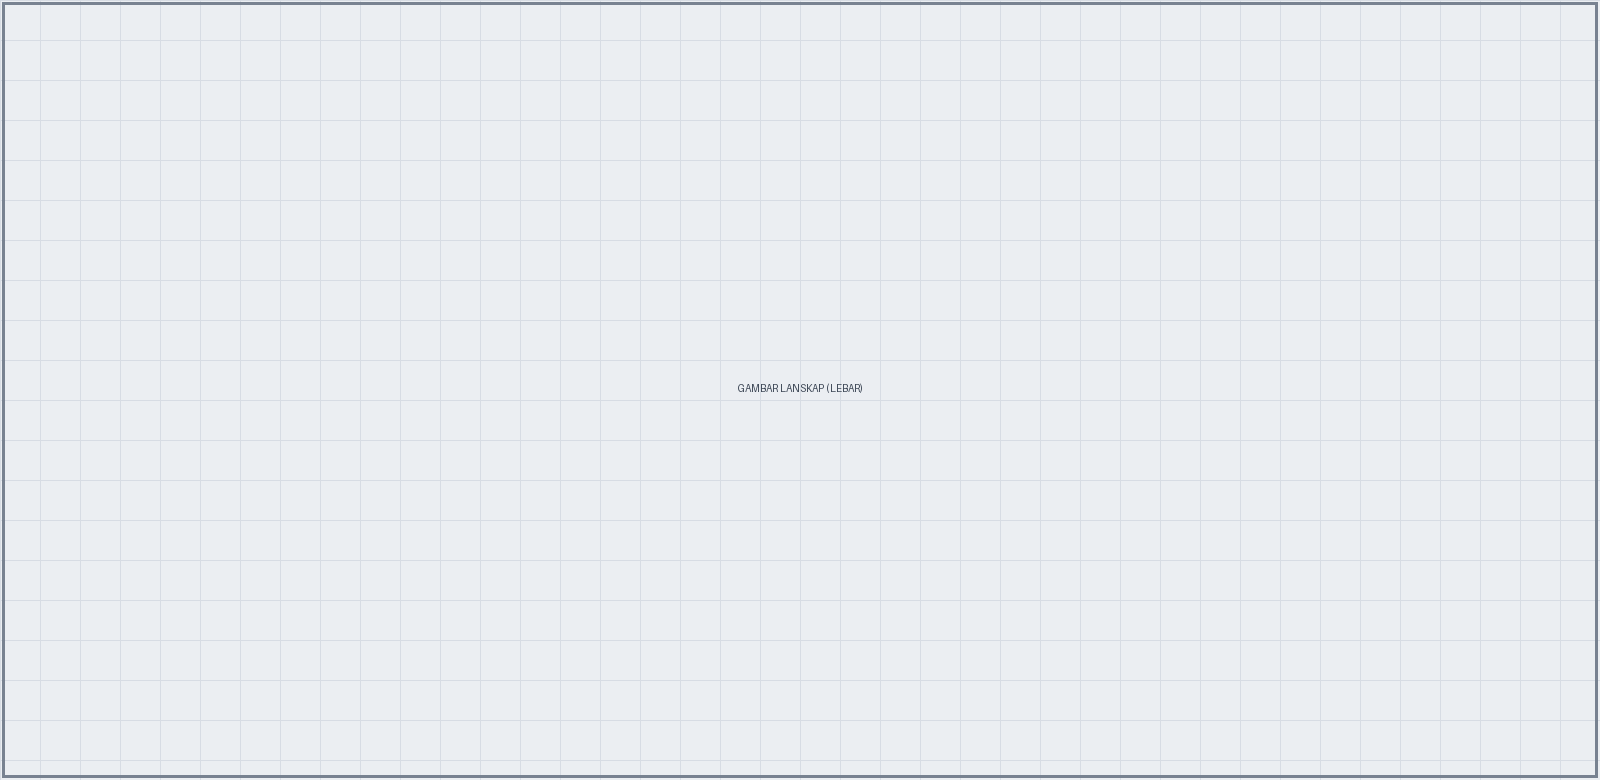
\includegraphics[width=0.92\linewidth]{contoh-lanskap}
    \caption{Contoh gambar pada halaman lanskap}
    \label{fig:g-lanskap}
\end{figure}
\end{landscape}

\subsection{Catatan penempatan gambar}
Parameter \texttt{[H]} memaksa gambar muncul tepat di posisi penulisannya.
Parameter \texttt{[htbp]} memberi LaTeX kebebasan menempatkan gambar pada
posisi terbaik, sehingga halaman tidak menyisakan ruang kosong. Gunakan
\texttt{[H]} bila urutan gambar penting, dan \texttt{[htbp]} bila
mengutamakan kerapian halaman.

% ==================================================================
\section{Persamaan}
% ==================================================================

Persamaan dalam baris teks ditulis seperti $\bar{x} = \sum x_i / n$, sedangkan
persamaan bernomor ditulis terpisah seperti \cref{eq:g-rerata}.

\begin{equation}
    \label{eq:g-rerata}
    \bar{x} = \frac{1}{n}\sum_{i=1}^{n} x_{i}
\end{equation}

Persamaan bertingkat ditulis dengan lingkungan \texttt{align}, dan setiap baris
memperoleh nomor tersendiri seperti \cref{eq:g-gap} dan \cref{eq:g-tki}.

\begin{align}
    \text{Gap}_i &= \bar{P}_i - \bar{I}_i \label{eq:g-gap} \\
    \text{TKI}_i &= \frac{\bar{P}_i}{\bar{I}_i} \times 100\% \label{eq:g-tki}
\end{align}

Beberapa bentuk yang sering dibutuhkan: pecahan $\frac{a}{b}$, akar
$\sqrt[3]{x}$, jumlah $\sum_{i=1}^{n}$, hasil kali $\prod_{i=1}^{n}$, integral
$\int_{0}^{1}$, huruf Yunani $\alpha, \beta, \sigma, \mu, \kappa$, serta matriks
berikut.

\begin{equation}
    \label{eq:g-matriks}
    \mathbf{D} =
    \begin{bmatrix}
        d_{11} & d_{12} & \cdots & d_{1n} \\
        d_{21} & d_{22} & \cdots & d_{2n} \\
        \vdots & \vdots & \ddots & \vdots \\
        d_{m1} & d_{m2} & \cdots & d_{mn}
    \end{bmatrix}
\end{equation}

% ==================================================================
\section{Kode Program}
% ==================================================================

\subsection{Kode ditulis langsung}
Kode dapat ditulis langsung di dalam naskah dan dirujuk seperti
\cref{lst:g-python}.

\begin{lstlisting}[language=Python, caption={Contoh kode Python}, label=lst:g-python]
def hitung_rerata(nilai):
    """Menghitung rata-rata dari sebuah senarai angka."""
    if not nilai:
        return 0
    return sum(nilai) / len(nilai)
\end{lstlisting}

\begin{lstlisting}[language=SQL, caption={Contoh kueri SQL}, label=lst:g-sql]
SELECT d.nama       AS dimensi,
       AVG(j.kinerja)     AS rerata_kinerja,
       AVG(j.kepentingan) AS rerata_penting
FROM   jawaban j
JOIN   butir b   ON b.id = j.butir_id
JOIN   dimensi d ON d.id = b.dimensi_id
GROUP  BY d.nama
ORDER  BY rerata_kinerja ASC;
\end{lstlisting}

\begin{lstlisting}[language=Java, caption={Contoh kode Java}, label=lst:g-java]
public class Responden {
    private final String kode;
    private final int[] jawaban;

    public Responden(String kode, int[] jawaban) {
        this.kode = kode;
        this.jawaban = jawaban;
    }

    public double rerata() {
        return Arrays.stream(jawaban)
                     .average()
                     .orElse(0.0);
    }
}
\end{lstlisting}

\begin{lstlisting}[language=PHP, caption={Contoh kode PHP}, label=lst:g-php]
<?php
function hitungGap(array $kin, array $pen): array {
    $gap = [];
    foreach ($kin as $b => $nilai) {
        $gap[$b] = round($nilai - $pen[$b], 2);
    }
    return $gap;
}
\end{lstlisting}

\subsection{Kode dibaca dari berkas}
Cara ini lebih dianjurkan untuk lampiran kode karena isinya selalu sinkron
dengan berkas sumber, dapat dicari, dan tidak membengkakkan ukuran berkas
seperti halnya tangkapan layar. Lihat \cref{lst:g-berkas}.

\lstinputlisting[language=Python, caption={Kode yang dibaca langsung dari berkas \texttt{kode/hitung-sus.py}}, label=lst:g-berkas]{kode/hitung-sus.py}

Sebagian baris saja juga dapat ditampilkan dengan parameter
\texttt{firstline} dan \texttt{lastline}.

\lstinputlisting[language=Python, firstline=7, lastline=18, caption={Cuplikan baris 7--18 dari berkas yang sama}, label=lst:g-cuplikan]{kode/hitung-sus.py}

\subsection{Pseudocode}
Untuk menuliskan algoritma, gunakan \texttt{algorithm2e}. Bentuk ini lebih
disukai penguji daripada kode nyata karena tidak terikat bahasa pemrograman
tertentu. Lihat \cref{alg:g-ipa}.

\begin{algorithm}[H]
\caption{Pemetaan kuadran \textit{Importance-Performance Analysis}}
\label{alg:g-ipa}
\KwMasukan{Senarai butir $B$, skor kepentingan $I$, skor kinerja $P$}
\KwKeluaran{Kuadran setiap butir}
$\bar{I} \leftarrow$ rata-rata seluruh nilai $I$\;
$\bar{P} \leftarrow$ rata-rata seluruh nilai $P$\;
\ForEach{butir $b \in B$}{
    \uIf{$I_b \geq \bar{I}$ \textbf{dan} $P_b < \bar{P}$}{
        $K_b \leftarrow$ ``Prioritas utama''\;
    }
    \uElseIf{$I_b \geq \bar{I}$}{
        $K_b \leftarrow$ ``Pertahankan prestasi''\;
    }
    \uElseIf{$P_b < \bar{P}$}{
        $K_b \leftarrow$ ``Prioritas rendah''\;
    }
    \Else{
        $K_b \leftarrow$ ``Berlebihan''\;
    }
}
\Return $K$\;
\end{algorithm}

% ==================================================================
\section{Sitasi dan Daftar Pustaka}
% ==================================================================

Template ini memakai gaya APA nama-tahun. Gaya diatur melalui perintah
\texttt{\textbackslash gayasitasi} pada berkas \texttt{a0-identitas.tex}.

\subsection{Bentuk sitasi}

\begin{daftarpoin}
    \item \texttt{\textbackslash citep\{kunci\}} menghasilkan sitasi dalam
          kurung: \citep{wijaya2022}. Dipakai bila rujukan bukan bagian dari
          kalimat.
    \item \texttt{\textbackslash citet\{kunci\}} menghasilkan sitasi naratif:
          \citet{wijaya2022}. Dipakai bila nama penulis menjadi subjek kalimat.
    \item Sitasi jamak ditulis dalam satu perintah:
          \citep{wijaya2022, pratama2023, sari2024}.
    \item Sitasi dengan halaman:
          \citep[hlm.~118]{barnes2002}.
    \item Sitasi dengan keterangan awalan:
          \citep[lihat][]{martilla1977}.
    \item Menyebut tahun saja: \citeyearpar{martilla1977}.
    \item Menyebut nama penulis saja: \citeauthor{barnes2002}.
\end{daftarpoin}

\subsection{Kutipan langsung}
Kutipan pendek ditulis menyatu dengan paragraf dan diapit tanda kutip.
Kutipan langsung yang panjang, yaitu lebih dari 40 kata, ditulis sebagai blok
tersendiri yang menjorok tanpa tanda kutip, seperti berikut.

\begin{quote}
    \noindent Tulis kutipan panjang Anda di sini. Blok kutipan ditulis menjorok
    ke dalam, tanpa tanda kutip, dan tetap diakhiri sitasi yang memuat nomor
    halaman sumbernya. Kutipan langsung sebaiknya digunakan seperlunya saja;
    utamakan parafrasa dengan bahasa Anda sendiri agar naskah tidak menjadi
    rangkaian kutipan. \citep[hlm.~120]{barnes2002}
\end{quote}

\subsection{Tipe entri pada berkas .bib}
Berkas \texttt{a7-pustaka.bib} memuat katalog seluruh tipe entri yang lazim
dipakai, yaitu \texttt{@article} untuk artikel jurnal, \texttt{@book} untuk
buku, \texttt{@incollection} untuk bab dalam bunga rampai,
\texttt{@inproceedings} untuk prosiding, \texttt{@mastersthesis} untuk skripsi
atau tesis, \texttt{@techreport} untuk laporan lembaga, \texttt{@manual} untuk
standar dan dokumentasi, serta \texttt{@misc} untuk sumber daring. Salin tipe
yang dibutuhkan lalu isi dengan data sebenarnya.

% Perintah \nocite berikut memaksa seluruh tipe entri ikut tampil pada
% Daftar Pustaka meskipun tidak disitasi di dalam teks, sehingga Anda
% dapat melihat bentuk tampilannya. Entri ini akan hilang sendiri
% begitu galeri dimatikan.
\nocite{contoh-buku, contoh-babbuku, contoh-prosiding, contoh-skripsi,
        contoh-laporan, contoh-standar, contoh-web}

Bentuk tampilan masing-masing tipe dapat Anda lihat langsung pada Daftar
Pustaka naskah ini.

% ==================================================================
\section{Rujukan Silang}
% ==================================================================

Seluruh rujukan silang sebaiknya memakai \texttt{\textbackslash cref} agar kata
``Gambar'', ``Tabel'', atau ``Persamaan'' muncul otomatis dan penomorannya
selalu sinkron: \cref{fig:g-tunggal}, \cref{tab:g-biasa}, \cref{eq:g-rerata},
\cref{lst:g-python}, dan \cref{alg:g-ipa}.

Beberapa objek sekaligus dapat dirujuk dalam satu perintah dan LaTeX akan
menyusun kata sambungnya sendiri: \cref{tab:g-biasa,tab:g-booktabs,tab:g-gabung}.

Rujukan ke rumusan masalah juga tersedia. Perintah \texttt{\textbackslash
cref\{rq:kualitas\}} menghasilkan \cref{rq:kualitas}, sehingga penomoran RQ di
seluruh naskah menyesuaikan sendiri bila urutannya diubah.
 di laporan.tex
% sebelum naskah dikumpulkan. Berkas ini tidak akan ikut tercetak,
% tetapi tetap tersimpan sebagai rujukan.
%==================================================================

% Galeri disertakan setelah lampiran, sehingga tanpa pengaturan ini
% penomorannya akan ikut melanjutkan huruf lampiran (D, E, dst.).
% Blok berikut membuatnya bernomor "G" agar jelas terpisah.
\clearpage
\setcounter{chapter}{0}
\setcounter{figure}{0}
\setcounter{table}{0}
\setcounter{equation}{0}
\renewcommand{\thechapter}{G}
\renewcommand{\thesection}{G.\arabic{section}}
\renewcommand{\thesubsection}{\thesection.\arabic{subsection}}
\renewcommand{\thefigure}{G.\arabic{figure}}
\renewcommand{\thetable}{G.\arabic{table}}
\renewcommand{\theequation}{G.\arabic{equation}}

\chapter*{GALERI ELEMEN (HAPUS SEBELUM DIKUMPULKAN)}
\addcontentsline{toc}{chapter}{GALERI ELEMEN (HAPUS SEBELUM DIKUMPULKAN)}

Bab ini bukan bagian dari naskah Tugas Akhir. Isinya adalah contoh siap salin
untuk seluruh elemen yang lazim dibutuhkan. Matikan dengan memberi tanda
\texttt{\%} pada baris \texttt{\textbackslash include\{zz-galeri-elemen\}} di
berkas \texttt{laporan.tex}.

% ==================================================================
\section{Tabel}
% ==================================================================

\subsection{Tabel biasa}
Keterangan tabel diletakkan di \textbf{atas} tabel. Setiap tabel wajib diberi
\texttt{\textbackslash label} dan disebut dalam teks, misalnya
\cref{tab:g-biasa}.

\begin{table}[H]
    \centering
    \caption{Contoh tabel biasa}
    \label{tab:g-biasa}
    \begin{tabular}{|c|l|c|}
        \hline
        \textbf{No} & \textbf{Keterangan} & \textbf{Nilai} \\ \hline
        1 & Baris pertama & 3,12 \\ \hline
        2 & Baris kedua   & 3,68 \\ \hline
        3 & Baris ketiga  & 3,54 \\ \hline
    \end{tabular}
\end{table}

\subsection{Tabel dengan garis gaya ilmiah (booktabs)}
Sebagian program studi menghendaki tabel tanpa garis vertikal.

\begin{table}[H]
    \centering
    \caption{Contoh tabel gaya booktabs}
    \label{tab:g-booktabs}
    \begin{tabular}{lcc}
        \toprule
        \textbf{Dimensi} & \textbf{Kepentingan} & \textbf{Kinerja} \\
        \midrule
        \textit{Usability}           & 4,41 & 3,12 \\
        \textit{Information quality} & 4,22 & 3,68 \\
        \bottomrule
    \end{tabular}
\end{table}

\subsection{Tabel bersambung antarhalaman (longtable)}
Gunakan \texttt{longtable} bila tabel lebih panjang daripada satu halaman.
Baris kepala akan diulang otomatis, dan halaman sambungan diberi keterangan
``Lanjutan'' sesuai kelaziman naskah Indonesia.

\begin{longtable}{|c|p{6.5cm}|c|c|}
    \caption{Contoh tabel bersambung antarhalaman}
    \label{tab:g-longtable} \\
    \hline
    \textbf{No} & \textbf{Pernyataan} & \textbf{Kepentingan} & \textbf{Kinerja} \\ \hline
    \endfirsthead

    \multicolumn{4}{l}{\footnotesize\textit{Lanjutan \cref{tab:g-longtable}}} \\
    \hline
    \textbf{No} & \textbf{Pernyataan} & \textbf{Kepentingan} & \textbf{Kinerja} \\ \hline
    \endhead

    \hline
    \multicolumn{4}{r}{\footnotesize\textit{Bersambung ke halaman berikutnya}} \\
    \endfoot

    \hline
    \endlastfoot

    1  & Saya merasa sistem mudah dipelajari & 4,44 & 3,10 \\ \hline
    2  & Interaksi dengan sistem jelas dan mudah dipahami & 4,38 & 3,21 \\ \hline
    3  & Sistem mudah dioperasikan & 4,41 & 3,15 \\ \hline
    4  & Navigasi antarhalaman terasa mudah & 4,61 & 3,03 \\ \hline
    5  & Tampilan sistem sesuai dengan jenis layanannya & 4,02 & 3,44 \\ \hline
    6  & Tampilan sistem menarik & 3,88 & 3,52 \\ \hline
    7  & Sistem menyampaikan kesan kompeten & 4,12 & 3,40 \\ \hline
    8  & Sistem menciptakan pengalaman yang menyenangkan & 3,95 & 3,33 \\ \hline
    9  & Informasi yang disajikan akurat & 4,30 & 3,71 \\ \hline
    10 & Informasi yang disajikan tepercaya & 4,28 & 3,69 \\ \hline
    11 & Informasi selalu diperbarui & 4,19 & 3,58 \\ \hline
    12 & Informasi relevan dengan kebutuhan & 4,25 & 3,66 \\ \hline
    13 & Informasi mudah dipahami & 4,21 & 3,74 \\ \hline
    14 & Informasi disajikan pada tingkat rincian yang tepat & 4,08 & 3,70 \\ \hline
    15 & Informasi disajikan dalam format yang sesuai & 4,15 & 3,68 \\ \hline
    16 & Sistem memberikan rasa aman & 4,09 & 3,61 \\ \hline
    17 & Data pribadi terasa terlindungi & 4,18 & 3,55 \\ \hline
    18 & Sistem memudahkan komunikasi dengan pengelola & 3,97 & 3,42 \\ \hline
    19 & Sistem menciptakan rasa keterhubungan & 3,82 & 3,39 \\ \hline
    20 & Layanan diberikan sesuai yang dijanjikan & 4,11 & 3,58 \\ \hline
\end{longtable}

\subsection{Tabel dengan sel gabung (multirow dan multicolumn)}

\begin{table}[H]
    \centering
    \caption{Contoh tabel dengan sel gabung}
    \label{tab:g-gabung}
    \begin{tabular}{|c|c|c|c|c|}
        \hline
        \multirow{2}{*}{\textbf{Butir}} & \multicolumn{2}{c|}{\textbf{Sebelum}} & \multicolumn{2}{c|}{\textbf{Sesudah}} \\ \cline{2-5}
         & \textbf{Rerata} & \textbf{SB} & \textbf{Rerata} & \textbf{SB} \\ \hline
        B1 & 3,10 & 0,82 & 4,05 & 0,61 \\ \hline
        B2 & 3,22 & 0,77 & 4,12 & 0,58 \\ \hline
    \end{tabular}
\end{table}

\subsection{Tabel berkolom otomatis (tabularx)}
Lebar kolom bertipe \texttt{X} menyesuaikan sendiri agar tabel tepat memenuhi
lebar teks.

\begin{table}[H]
    \centering
    \caption{Contoh tabel dengan lebar kolom otomatis}
    \label{tab:g-tabularx}
    \begin{tabularx}{\textwidth}{|c|X|X|}
        \hline
        \textbf{No} & \textbf{Temuan} & \textbf{Tindak lanjut} \\ \hline
        1 & Menu utama tidak konsisten antarhalaman sehingga pengguna kehilangan orientasi. & Menyeragamkan struktur menu pada seluruh halaman. \\ \hline
        2 & Pesan kesalahan tidak menjelaskan penyebab masalah. & Menulis ulang pesan kesalahan dengan bahasa yang spesifik. \\ \hline
    \end{tabularx}
\end{table}

\subsection{Tabel dengan catatan kaki (threeparttable)}
Gunakan bila tabel memerlukan keterangan simbol atau sumber.

\begin{table}[H]
    \centering
    \begin{threeparttable}
        \caption{Contoh tabel dengan catatan kaki}
        \label{tab:g-catatan}
        \begin{tabular}{|l|c|c|}
            \hline
            \textbf{Dimensi} & \textbf{Rerata} & \textbf{Kategori} \\ \hline
            \textit{Usability}\tnote{a}           & 3,12 & Cukup \\ \hline
            \textit{Information quality}          & 3,68 & Baik  \\ \hline
            \textit{Service interaction}\tnote{b} & 3,54 & Baik  \\ \hline
        \end{tabular}
        \begin{tablenotes}\footnotesize
            \item[a] Terdiri atas 8 butir pernyataan.
            \item[b] Terdiri atas 7 butir pernyataan.
            \item Sumber: Hasil pengolahan data penelitian (2026).
        \end{tablenotes}
    \end{threeparttable}
\end{table}

\subsection{Tabel yang terlalu lebar}
Bila tabel sedikit melebihi lebar teks, perkecil jarak antarkolom dengan
\texttt{\textbackslash tabcolsep} atau bungkus dengan \texttt{adjustbox}.

\begin{table}[H]
    \centering
    \caption{Contoh tabel lebar yang dikecilkan otomatis}
    \label{tab:g-lebar}
    \footnotesize
    \begin{adjustbox}{max width=\textwidth}
    \begin{tabular}{|c|c|c|c|c|c|c|c|c|c|c|}
        \hline
        \textbf{Butir} & \textbf{R1} & \textbf{R2} & \textbf{R3} & \textbf{R4} & \textbf{R5} & \textbf{R6} & \textbf{R7} & \textbf{R8} & \textbf{Rerata} & \textbf{Simpangan Baku} \\ \hline
        B1 & 4 & 5 & 4 & 3 & 4 & 5 & 4 & 4 & 4,13 & 0,64 \\ \hline
        B2 & 3 & 4 & 4 & 4 & 5 & 4 & 3 & 4 & 3,88 & 0,64 \\ \hline
    \end{tabular}
    \end{adjustbox}
\end{table}

\subsection{Tabel lanskap}
Paket \texttt{pdflscape} ikut memutar halaman pada berkas PDF, sehingga pembaca
tidak perlu memiringkan kepala.

\begin{landscape}
\begin{table}[H]
    \centering
    \caption{Contoh tabel pada halaman lanskap}
    \label{tab:g-lanskap}
    \footnotesize
    \begin{tabular}{|c|p{4cm}|p{4cm}|p{4cm}|p{4cm}|}
        \hline
        \textbf{No} & \textbf{Kondisi berjalan} & \textbf{Masalah} & \textbf{Usulan} & \textbf{Dampak yang diharapkan} \\ \hline
        1 & Menu tersebar pada tiga tingkat & Pengguna kesulitan menemukan menu & Menyusun ulang menjadi dua tingkat & Waktu pencarian menu berkurang \\ \hline
        2 & Alur pengisian tidak menampilkan tahapan & Pengguna tidak tahu posisinya & Menambahkan penanda tahapan & Kesalahan pengisian berkurang \\ \hline
    \end{tabular}
\end{table}
\end{landscape}

% ==================================================================
\section{Gambar}
% ==================================================================

\subsection{Gambar tunggal}
Keterangan gambar diletakkan di \textbf{bawah} gambar. Lihat
\cref{fig:g-tunggal}.

\begin{figure}[H]
    \centering
    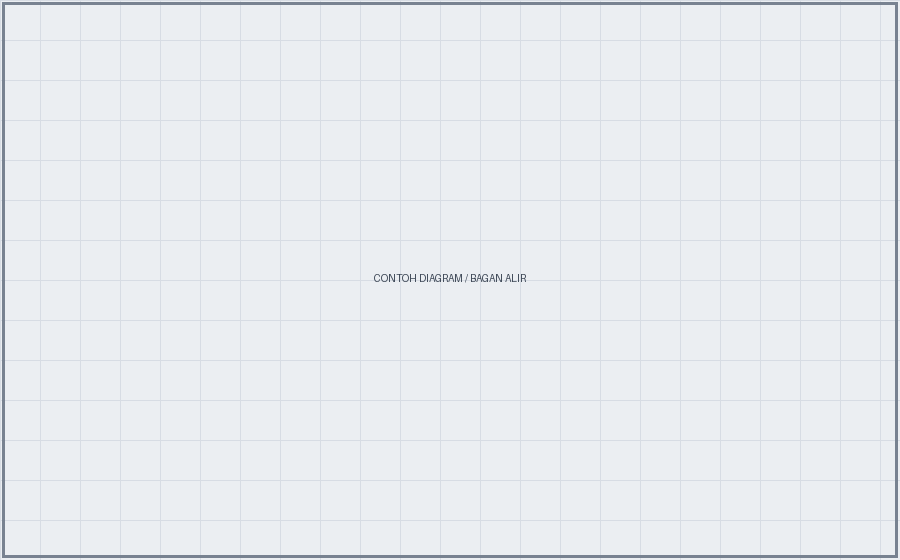
\includegraphics[width=0.6\linewidth]{contoh-diagram}
    \caption{Contoh gambar tunggal}
    \label{fig:g-tunggal}
\end{figure}

\subsection{Gambar dengan keterangan sumber}
Gunakan perintah \texttt{\textbackslash sumber} bila gambar dikutip dari
sumber lain.

\begin{figure}[H]
    \centering
    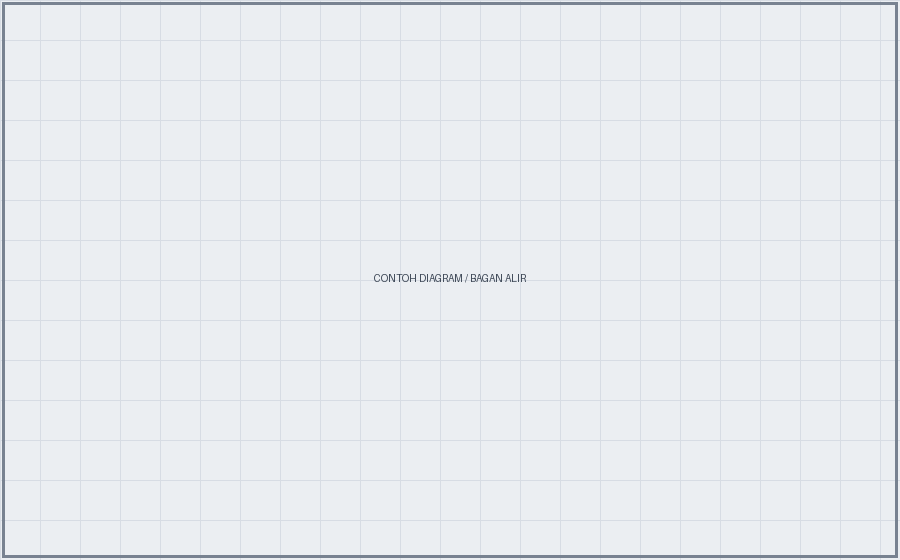
\includegraphics[width=0.55\linewidth]{contoh-diagram}
    \caption{Contoh gambar yang dikutip dari sumber lain}
    \label{fig:g-sumber}
\end{figure}
\sumber{\citet{barnes2002}}

\subsection{Dua gambar berdampingan}
Gunakan \texttt{subcaption} agar tiap bagian memperoleh label (a) dan (b) yang
dapat dirujuk terpisah, misalnya \cref{fig:g-kiri} dan \cref{fig:g-kanan}.

\begin{figure}[H]
    \centering
    \begin{subfigure}[t]{0.47\linewidth}
        \centering
        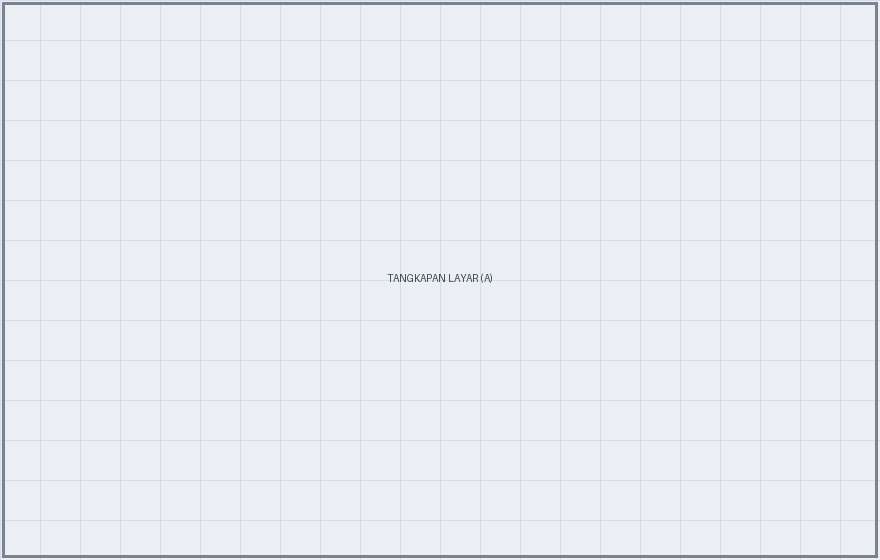
\includegraphics[width=\linewidth]{contoh-tangkapan-a}
        \caption{Tampilan sebelum perbaikan}
        \label{fig:g-kiri}
    \end{subfigure}
    \hfill
    \begin{subfigure}[t]{0.47\linewidth}
        \centering
        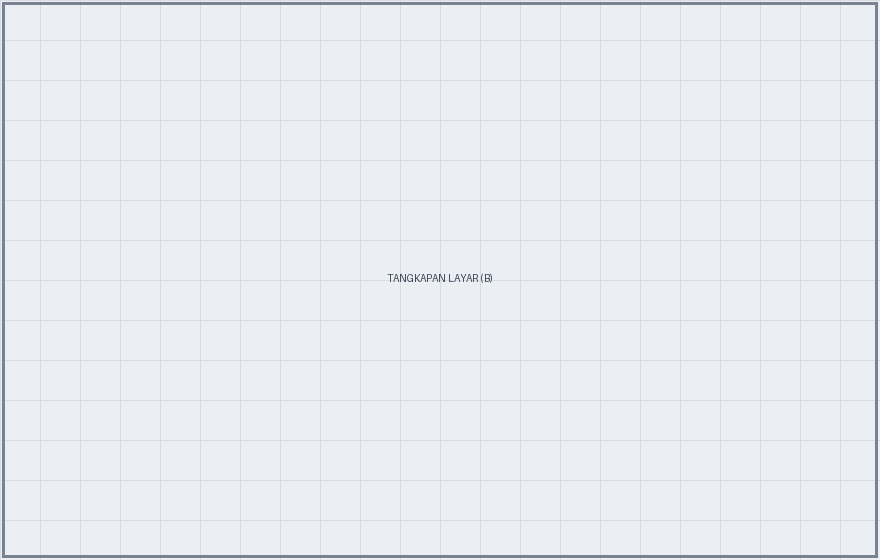
\includegraphics[width=\linewidth]{contoh-tangkapan-b}
        \caption{Tampilan sesudah perbaikan}
        \label{fig:g-kanan}
    \end{subfigure}
    \caption{Perbandingan tampilan antarmuka}
    \label{fig:g-berdampingan}
\end{figure}

\subsection{Gambar tinggi satu halaman}
Untuk gambar yang tinggi, seperti diagram alir panjang, gunakan
\texttt{height} agar tidak meluber ke halaman berikutnya.

\begin{figure}[H]
    \centering
    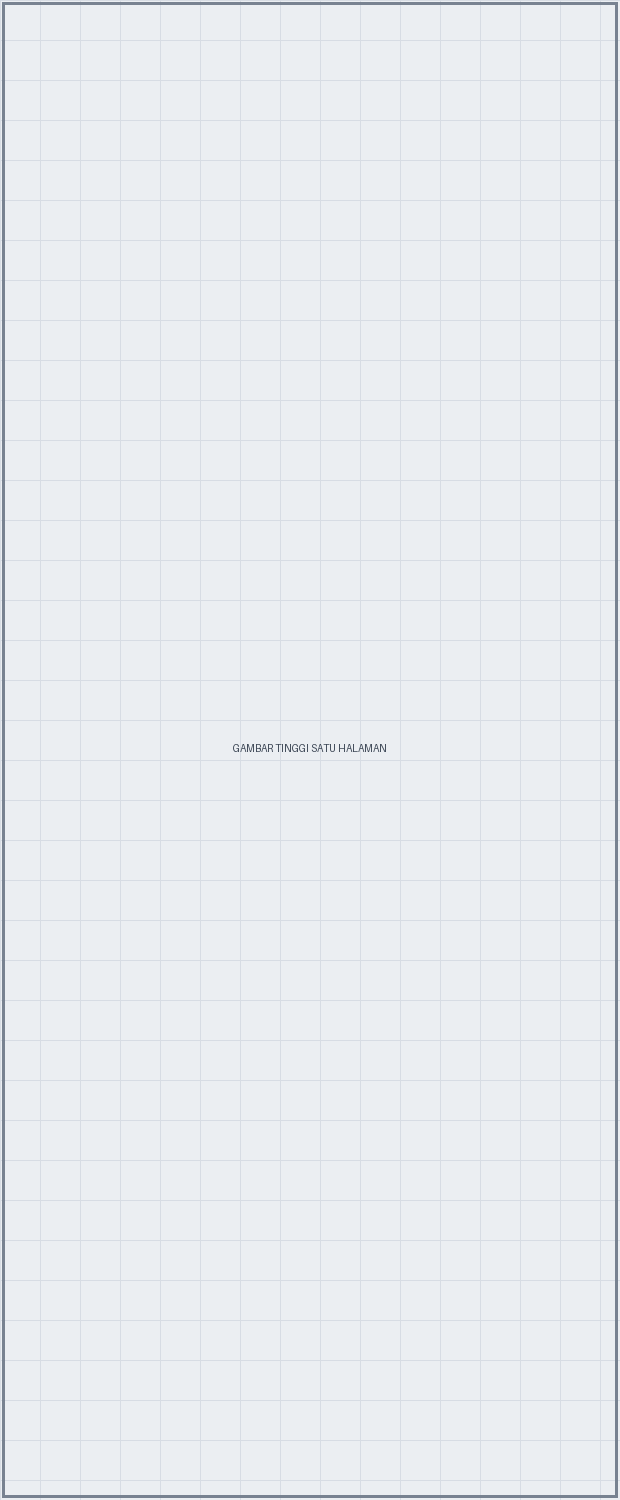
\includegraphics[height=0.78\textheight,keepaspectratio]{contoh-tinggi}
    \caption{Contoh gambar tinggi satu halaman}
    \label{fig:g-tinggi}
\end{figure}

\subsection{Gambar lanskap}

\begin{landscape}
\begin{figure}[H]
    \centering
    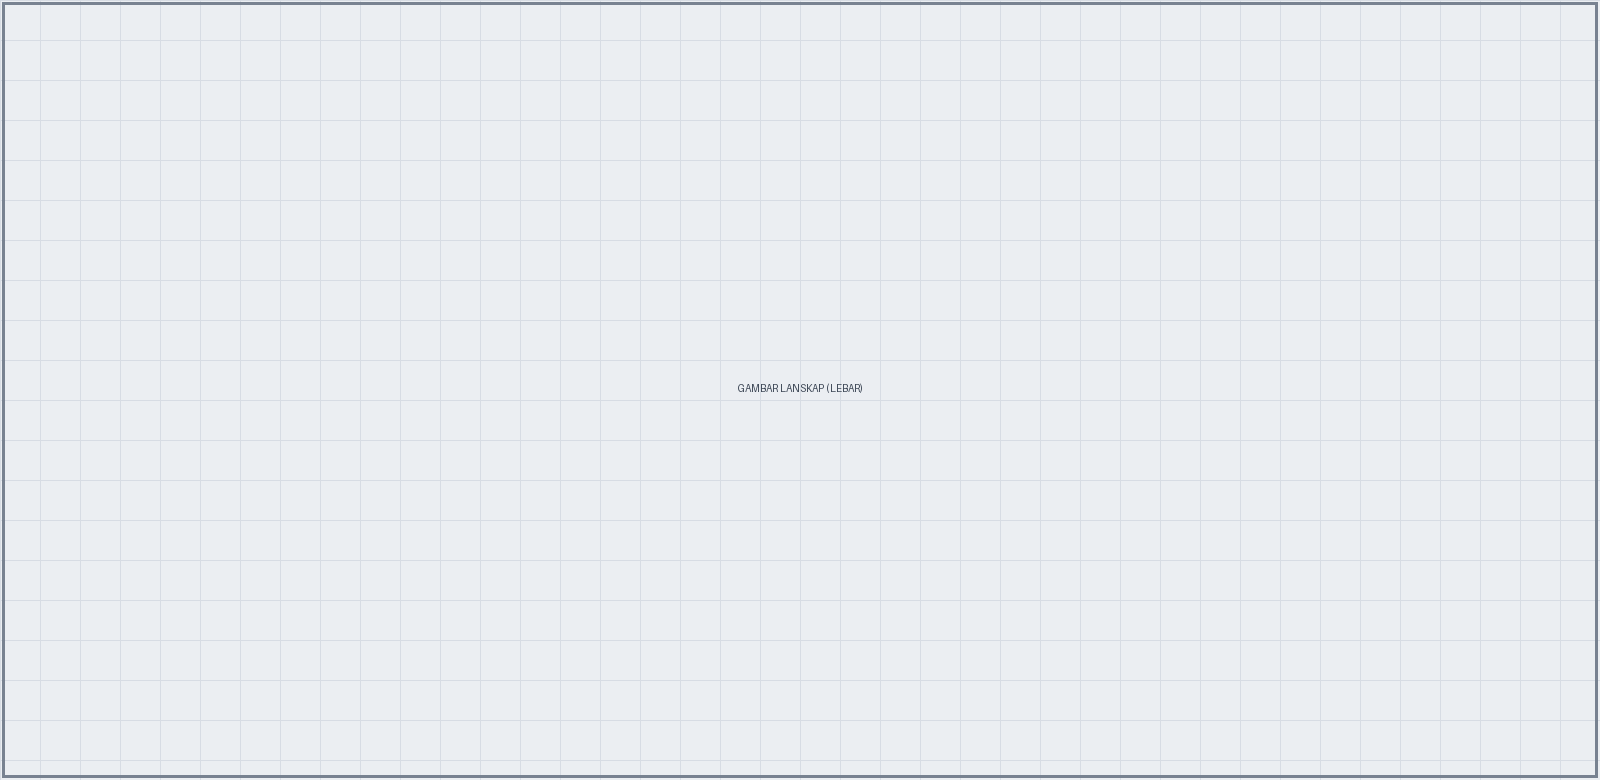
\includegraphics[width=0.92\linewidth]{contoh-lanskap}
    \caption{Contoh gambar pada halaman lanskap}
    \label{fig:g-lanskap}
\end{figure}
\end{landscape}

\subsection{Catatan penempatan gambar}
Parameter \texttt{[H]} memaksa gambar muncul tepat di posisi penulisannya.
Parameter \texttt{[htbp]} memberi LaTeX kebebasan menempatkan gambar pada
posisi terbaik, sehingga halaman tidak menyisakan ruang kosong. Gunakan
\texttt{[H]} bila urutan gambar penting, dan \texttt{[htbp]} bila
mengutamakan kerapian halaman.

% ==================================================================
\section{Persamaan}
% ==================================================================

Persamaan dalam baris teks ditulis seperti $\bar{x} = \sum x_i / n$, sedangkan
persamaan bernomor ditulis terpisah seperti \cref{eq:g-rerata}.

\begin{equation}
    \label{eq:g-rerata}
    \bar{x} = \frac{1}{n}\sum_{i=1}^{n} x_{i}
\end{equation}

Persamaan bertingkat ditulis dengan lingkungan \texttt{align}, dan setiap baris
memperoleh nomor tersendiri seperti \cref{eq:g-gap} dan \cref{eq:g-tki}.

\begin{align}
    \text{Gap}_i &= \bar{P}_i - \bar{I}_i \label{eq:g-gap} \\
    \text{TKI}_i &= \frac{\bar{P}_i}{\bar{I}_i} \times 100\% \label{eq:g-tki}
\end{align}

Beberapa bentuk yang sering dibutuhkan: pecahan $\frac{a}{b}$, akar
$\sqrt[3]{x}$, jumlah $\sum_{i=1}^{n}$, hasil kali $\prod_{i=1}^{n}$, integral
$\int_{0}^{1}$, huruf Yunani $\alpha, \beta, \sigma, \mu, \kappa$, serta matriks
berikut.

\begin{equation}
    \label{eq:g-matriks}
    \mathbf{D} =
    \begin{bmatrix}
        d_{11} & d_{12} & \cdots & d_{1n} \\
        d_{21} & d_{22} & \cdots & d_{2n} \\
        \vdots & \vdots & \ddots & \vdots \\
        d_{m1} & d_{m2} & \cdots & d_{mn}
    \end{bmatrix}
\end{equation}

% ==================================================================
\section{Kode Program}
% ==================================================================

\subsection{Kode ditulis langsung}
Kode dapat ditulis langsung di dalam naskah dan dirujuk seperti
\cref{lst:g-python}.

\begin{lstlisting}[language=Python, caption={Contoh kode Python}, label=lst:g-python]
def hitung_rerata(nilai):
    """Menghitung rata-rata dari sebuah senarai angka."""
    if not nilai:
        return 0
    return sum(nilai) / len(nilai)
\end{lstlisting}

\begin{lstlisting}[language=SQL, caption={Contoh kueri SQL}, label=lst:g-sql]
SELECT d.nama       AS dimensi,
       AVG(j.kinerja)     AS rerata_kinerja,
       AVG(j.kepentingan) AS rerata_penting
FROM   jawaban j
JOIN   butir b   ON b.id = j.butir_id
JOIN   dimensi d ON d.id = b.dimensi_id
GROUP  BY d.nama
ORDER  BY rerata_kinerja ASC;
\end{lstlisting}

\begin{lstlisting}[language=Java, caption={Contoh kode Java}, label=lst:g-java]
public class Responden {
    private final String kode;
    private final int[] jawaban;

    public Responden(String kode, int[] jawaban) {
        this.kode = kode;
        this.jawaban = jawaban;
    }

    public double rerata() {
        return Arrays.stream(jawaban)
                     .average()
                     .orElse(0.0);
    }
}
\end{lstlisting}

\begin{lstlisting}[language=PHP, caption={Contoh kode PHP}, label=lst:g-php]
<?php
function hitungGap(array $kin, array $pen): array {
    $gap = [];
    foreach ($kin as $b => $nilai) {
        $gap[$b] = round($nilai - $pen[$b], 2);
    }
    return $gap;
}
\end{lstlisting}

\subsection{Kode dibaca dari berkas}
Cara ini lebih dianjurkan untuk lampiran kode karena isinya selalu sinkron
dengan berkas sumber, dapat dicari, dan tidak membengkakkan ukuran berkas
seperti halnya tangkapan layar. Lihat \cref{lst:g-berkas}.

\lstinputlisting[language=Python, caption={Kode yang dibaca langsung dari berkas \texttt{kode/hitung-sus.py}}, label=lst:g-berkas]{kode/hitung-sus.py}

Sebagian baris saja juga dapat ditampilkan dengan parameter
\texttt{firstline} dan \texttt{lastline}.

\lstinputlisting[language=Python, firstline=7, lastline=18, caption={Cuplikan baris 7--18 dari berkas yang sama}, label=lst:g-cuplikan]{kode/hitung-sus.py}

\subsection{Pseudocode}
Untuk menuliskan algoritma, gunakan \texttt{algorithm2e}. Bentuk ini lebih
disukai penguji daripada kode nyata karena tidak terikat bahasa pemrograman
tertentu. Lihat \cref{alg:g-ipa}.

\begin{algorithm}[H]
\caption{Pemetaan kuadran \textit{Importance-Performance Analysis}}
\label{alg:g-ipa}
\KwMasukan{Senarai butir $B$, skor kepentingan $I$, skor kinerja $P$}
\KwKeluaran{Kuadran setiap butir}
$\bar{I} \leftarrow$ rata-rata seluruh nilai $I$\;
$\bar{P} \leftarrow$ rata-rata seluruh nilai $P$\;
\ForEach{butir $b \in B$}{
    \uIf{$I_b \geq \bar{I}$ \textbf{dan} $P_b < \bar{P}$}{
        $K_b \leftarrow$ ``Prioritas utama''\;
    }
    \uElseIf{$I_b \geq \bar{I}$}{
        $K_b \leftarrow$ ``Pertahankan prestasi''\;
    }
    \uElseIf{$P_b < \bar{P}$}{
        $K_b \leftarrow$ ``Prioritas rendah''\;
    }
    \Else{
        $K_b \leftarrow$ ``Berlebihan''\;
    }
}
\Return $K$\;
\end{algorithm}

% ==================================================================
\section{Sitasi dan Daftar Pustaka}
% ==================================================================

Template ini memakai gaya APA nama-tahun. Gaya diatur melalui perintah
\texttt{\textbackslash gayasitasi} pada berkas \texttt{a0-identitas.tex}.

\subsection{Bentuk sitasi}

\begin{daftarpoin}
    \item \texttt{\textbackslash citep\{kunci\}} menghasilkan sitasi dalam
          kurung: \citep{wijaya2022}. Dipakai bila rujukan bukan bagian dari
          kalimat.
    \item \texttt{\textbackslash citet\{kunci\}} menghasilkan sitasi naratif:
          \citet{wijaya2022}. Dipakai bila nama penulis menjadi subjek kalimat.
    \item Sitasi jamak ditulis dalam satu perintah:
          \citep{wijaya2022, pratama2023, sari2024}.
    \item Sitasi dengan halaman:
          \citep[hlm.~118]{barnes2002}.
    \item Sitasi dengan keterangan awalan:
          \citep[lihat][]{martilla1977}.
    \item Menyebut tahun saja: \citeyearpar{martilla1977}.
    \item Menyebut nama penulis saja: \citeauthor{barnes2002}.
\end{daftarpoin}

\subsection{Kutipan langsung}
Kutipan pendek ditulis menyatu dengan paragraf dan diapit tanda kutip.
Kutipan langsung yang panjang, yaitu lebih dari 40 kata, ditulis sebagai blok
tersendiri yang menjorok tanpa tanda kutip, seperti berikut.

\begin{quote}
    \noindent Tulis kutipan panjang Anda di sini. Blok kutipan ditulis menjorok
    ke dalam, tanpa tanda kutip, dan tetap diakhiri sitasi yang memuat nomor
    halaman sumbernya. Kutipan langsung sebaiknya digunakan seperlunya saja;
    utamakan parafrasa dengan bahasa Anda sendiri agar naskah tidak menjadi
    rangkaian kutipan. \citep[hlm.~120]{barnes2002}
\end{quote}

\subsection{Tipe entri pada berkas .bib}
Berkas \texttt{a7-pustaka.bib} memuat katalog seluruh tipe entri yang lazim
dipakai, yaitu \texttt{@article} untuk artikel jurnal, \texttt{@book} untuk
buku, \texttt{@incollection} untuk bab dalam bunga rampai,
\texttt{@inproceedings} untuk prosiding, \texttt{@mastersthesis} untuk skripsi
atau tesis, \texttt{@techreport} untuk laporan lembaga, \texttt{@manual} untuk
standar dan dokumentasi, serta \texttt{@misc} untuk sumber daring. Salin tipe
yang dibutuhkan lalu isi dengan data sebenarnya.

% Perintah \nocite berikut memaksa seluruh tipe entri ikut tampil pada
% Daftar Pustaka meskipun tidak disitasi di dalam teks, sehingga Anda
% dapat melihat bentuk tampilannya. Entri ini akan hilang sendiri
% begitu galeri dimatikan.
\nocite{contoh-buku, contoh-babbuku, contoh-prosiding, contoh-skripsi,
        contoh-laporan, contoh-standar, contoh-web}

Bentuk tampilan masing-masing tipe dapat Anda lihat langsung pada Daftar
Pustaka naskah ini.

% ==================================================================
\section{Rujukan Silang}
% ==================================================================

Seluruh rujukan silang sebaiknya memakai \texttt{\textbackslash cref} agar kata
``Gambar'', ``Tabel'', atau ``Persamaan'' muncul otomatis dan penomorannya
selalu sinkron: \cref{fig:g-tunggal}, \cref{tab:g-biasa}, \cref{eq:g-rerata},
\cref{lst:g-python}, dan \cref{alg:g-ipa}.

Beberapa objek sekaligus dapat dirujuk dalam satu perintah dan LaTeX akan
menyusun kata sambungnya sendiri: \cref{tab:g-biasa,tab:g-booktabs,tab:g-gabung}.

Rujukan ke rumusan masalah juga tersedia. Perintah \texttt{\textbackslash
cref\{rq:kualitas\}} menghasilkan \cref{rq:kualitas}, sehingga penomoran RQ di
seluruh naskah menyesuaikan sendiri bila urutannya diubah.
 di laporan.tex
% sebelum naskah dikumpulkan. Berkas ini tidak akan ikut tercetak,
% tetapi tetap tersimpan sebagai rujukan.
%==================================================================

% Galeri disertakan setelah lampiran, sehingga tanpa pengaturan ini
% penomorannya akan ikut melanjutkan huruf lampiran (D, E, dst.).
% Blok berikut membuatnya bernomor "G" agar jelas terpisah.
\clearpage
\setcounter{chapter}{0}
\setcounter{figure}{0}
\setcounter{table}{0}
\setcounter{equation}{0}
\renewcommand{\thechapter}{G}
\renewcommand{\thesection}{G.\arabic{section}}
\renewcommand{\thesubsection}{\thesection.\arabic{subsection}}
\renewcommand{\thefigure}{G.\arabic{figure}}
\renewcommand{\thetable}{G.\arabic{table}}
\renewcommand{\theequation}{G.\arabic{equation}}

\chapter*{GALERI ELEMEN (HAPUS SEBELUM DIKUMPULKAN)}
\addcontentsline{toc}{chapter}{GALERI ELEMEN (HAPUS SEBELUM DIKUMPULKAN)}

Bab ini bukan bagian dari naskah Tugas Akhir. Isinya adalah contoh siap salin
untuk seluruh elemen yang lazim dibutuhkan. Matikan dengan memberi tanda
\texttt{\%} pada baris \texttt{\textbackslash include\{zz-galeri-elemen\}} di
berkas \texttt{laporan.tex}.

% ==================================================================
\section{Tabel}
% ==================================================================

\subsection{Tabel biasa}
Keterangan tabel diletakkan di \textbf{atas} tabel. Setiap tabel wajib diberi
\texttt{\textbackslash label} dan disebut dalam teks, misalnya
\cref{tab:g-biasa}.

\begin{table}[H]
    \centering
    \caption{Contoh tabel biasa}
    \label{tab:g-biasa}
    \begin{tabular}{|c|l|c|}
        \hline
        \textbf{No} & \textbf{Keterangan} & \textbf{Nilai} \\ \hline
        1 & Baris pertama & 3,12 \\ \hline
        2 & Baris kedua   & 3,68 \\ \hline
        3 & Baris ketiga  & 3,54 \\ \hline
    \end{tabular}
\end{table}

\subsection{Tabel dengan garis gaya ilmiah (booktabs)}
Sebagian program studi menghendaki tabel tanpa garis vertikal.

\begin{table}[H]
    \centering
    \caption{Contoh tabel gaya booktabs}
    \label{tab:g-booktabs}
    \begin{tabular}{lcc}
        \toprule
        \textbf{Dimensi} & \textbf{Kepentingan} & \textbf{Kinerja} \\
        \midrule
        \textit{Usability}           & 4,41 & 3,12 \\
        \textit{Information quality} & 4,22 & 3,68 \\
        \bottomrule
    \end{tabular}
\end{table}

\subsection{Tabel bersambung antarhalaman (longtable)}
Gunakan \texttt{longtable} bila tabel lebih panjang daripada satu halaman.
Baris kepala akan diulang otomatis, dan halaman sambungan diberi keterangan
``Lanjutan'' sesuai kelaziman naskah Indonesia.

\begin{longtable}{|c|p{6.5cm}|c|c|}
    \caption{Contoh tabel bersambung antarhalaman}
    \label{tab:g-longtable} \\
    \hline
    \textbf{No} & \textbf{Pernyataan} & \textbf{Kepentingan} & \textbf{Kinerja} \\ \hline
    \endfirsthead

    \multicolumn{4}{l}{\footnotesize\textit{Lanjutan \cref{tab:g-longtable}}} \\
    \hline
    \textbf{No} & \textbf{Pernyataan} & \textbf{Kepentingan} & \textbf{Kinerja} \\ \hline
    \endhead

    \hline
    \multicolumn{4}{r}{\footnotesize\textit{Bersambung ke halaman berikutnya}} \\
    \endfoot

    \hline
    \endlastfoot

    1  & Saya merasa sistem mudah dipelajari & 4,44 & 3,10 \\ \hline
    2  & Interaksi dengan sistem jelas dan mudah dipahami & 4,38 & 3,21 \\ \hline
    3  & Sistem mudah dioperasikan & 4,41 & 3,15 \\ \hline
    4  & Navigasi antarhalaman terasa mudah & 4,61 & 3,03 \\ \hline
    5  & Tampilan sistem sesuai dengan jenis layanannya & 4,02 & 3,44 \\ \hline
    6  & Tampilan sistem menarik & 3,88 & 3,52 \\ \hline
    7  & Sistem menyampaikan kesan kompeten & 4,12 & 3,40 \\ \hline
    8  & Sistem menciptakan pengalaman yang menyenangkan & 3,95 & 3,33 \\ \hline
    9  & Informasi yang disajikan akurat & 4,30 & 3,71 \\ \hline
    10 & Informasi yang disajikan tepercaya & 4,28 & 3,69 \\ \hline
    11 & Informasi selalu diperbarui & 4,19 & 3,58 \\ \hline
    12 & Informasi relevan dengan kebutuhan & 4,25 & 3,66 \\ \hline
    13 & Informasi mudah dipahami & 4,21 & 3,74 \\ \hline
    14 & Informasi disajikan pada tingkat rincian yang tepat & 4,08 & 3,70 \\ \hline
    15 & Informasi disajikan dalam format yang sesuai & 4,15 & 3,68 \\ \hline
    16 & Sistem memberikan rasa aman & 4,09 & 3,61 \\ \hline
    17 & Data pribadi terasa terlindungi & 4,18 & 3,55 \\ \hline
    18 & Sistem memudahkan komunikasi dengan pengelola & 3,97 & 3,42 \\ \hline
    19 & Sistem menciptakan rasa keterhubungan & 3,82 & 3,39 \\ \hline
    20 & Layanan diberikan sesuai yang dijanjikan & 4,11 & 3,58 \\ \hline
\end{longtable}

\subsection{Tabel dengan sel gabung (multirow dan multicolumn)}

\begin{table}[H]
    \centering
    \caption{Contoh tabel dengan sel gabung}
    \label{tab:g-gabung}
    \begin{tabular}{|c|c|c|c|c|}
        \hline
        \multirow{2}{*}{\textbf{Butir}} & \multicolumn{2}{c|}{\textbf{Sebelum}} & \multicolumn{2}{c|}{\textbf{Sesudah}} \\ \cline{2-5}
         & \textbf{Rerata} & \textbf{SB} & \textbf{Rerata} & \textbf{SB} \\ \hline
        B1 & 3,10 & 0,82 & 4,05 & 0,61 \\ \hline
        B2 & 3,22 & 0,77 & 4,12 & 0,58 \\ \hline
    \end{tabular}
\end{table}

\subsection{Tabel berkolom otomatis (tabularx)}
Lebar kolom bertipe \texttt{X} menyesuaikan sendiri agar tabel tepat memenuhi
lebar teks.

\begin{table}[H]
    \centering
    \caption{Contoh tabel dengan lebar kolom otomatis}
    \label{tab:g-tabularx}
    \begin{tabularx}{\textwidth}{|c|X|X|}
        \hline
        \textbf{No} & \textbf{Temuan} & \textbf{Tindak lanjut} \\ \hline
        1 & Menu utama tidak konsisten antarhalaman sehingga pengguna kehilangan orientasi. & Menyeragamkan struktur menu pada seluruh halaman. \\ \hline
        2 & Pesan kesalahan tidak menjelaskan penyebab masalah. & Menulis ulang pesan kesalahan dengan bahasa yang spesifik. \\ \hline
    \end{tabularx}
\end{table}

\subsection{Tabel dengan catatan kaki (threeparttable)}
Gunakan bila tabel memerlukan keterangan simbol atau sumber.

\begin{table}[H]
    \centering
    \begin{threeparttable}
        \caption{Contoh tabel dengan catatan kaki}
        \label{tab:g-catatan}
        \begin{tabular}{|l|c|c|}
            \hline
            \textbf{Dimensi} & \textbf{Rerata} & \textbf{Kategori} \\ \hline
            \textit{Usability}\tnote{a}           & 3,12 & Cukup \\ \hline
            \textit{Information quality}          & 3,68 & Baik  \\ \hline
            \textit{Service interaction}\tnote{b} & 3,54 & Baik  \\ \hline
        \end{tabular}
        \begin{tablenotes}\footnotesize
            \item[a] Terdiri atas 8 butir pernyataan.
            \item[b] Terdiri atas 7 butir pernyataan.
            \item Sumber: Hasil pengolahan data penelitian (2026).
        \end{tablenotes}
    \end{threeparttable}
\end{table}

\subsection{Tabel yang terlalu lebar}
Bila tabel sedikit melebihi lebar teks, perkecil jarak antarkolom dengan
\texttt{\textbackslash tabcolsep} atau bungkus dengan \texttt{adjustbox}.

\begin{table}[H]
    \centering
    \caption{Contoh tabel lebar yang dikecilkan otomatis}
    \label{tab:g-lebar}
    \footnotesize
    \begin{adjustbox}{max width=\textwidth}
    \begin{tabular}{|c|c|c|c|c|c|c|c|c|c|c|}
        \hline
        \textbf{Butir} & \textbf{R1} & \textbf{R2} & \textbf{R3} & \textbf{R4} & \textbf{R5} & \textbf{R6} & \textbf{R7} & \textbf{R8} & \textbf{Rerata} & \textbf{Simpangan Baku} \\ \hline
        B1 & 4 & 5 & 4 & 3 & 4 & 5 & 4 & 4 & 4,13 & 0,64 \\ \hline
        B2 & 3 & 4 & 4 & 4 & 5 & 4 & 3 & 4 & 3,88 & 0,64 \\ \hline
    \end{tabular}
    \end{adjustbox}
\end{table}

\subsection{Tabel lanskap}
Paket \texttt{pdflscape} ikut memutar halaman pada berkas PDF, sehingga pembaca
tidak perlu memiringkan kepala.

\begin{landscape}
\begin{table}[H]
    \centering
    \caption{Contoh tabel pada halaman lanskap}
    \label{tab:g-lanskap}
    \footnotesize
    \begin{tabular}{|c|p{4cm}|p{4cm}|p{4cm}|p{4cm}|}
        \hline
        \textbf{No} & \textbf{Kondisi berjalan} & \textbf{Masalah} & \textbf{Usulan} & \textbf{Dampak yang diharapkan} \\ \hline
        1 & Menu tersebar pada tiga tingkat & Pengguna kesulitan menemukan menu & Menyusun ulang menjadi dua tingkat & Waktu pencarian menu berkurang \\ \hline
        2 & Alur pengisian tidak menampilkan tahapan & Pengguna tidak tahu posisinya & Menambahkan penanda tahapan & Kesalahan pengisian berkurang \\ \hline
    \end{tabular}
\end{table}
\end{landscape}

% ==================================================================
\section{Gambar}
% ==================================================================

\subsection{Gambar tunggal}
Keterangan gambar diletakkan di \textbf{bawah} gambar. Lihat
\cref{fig:g-tunggal}.

\begin{figure}[H]
    \centering
    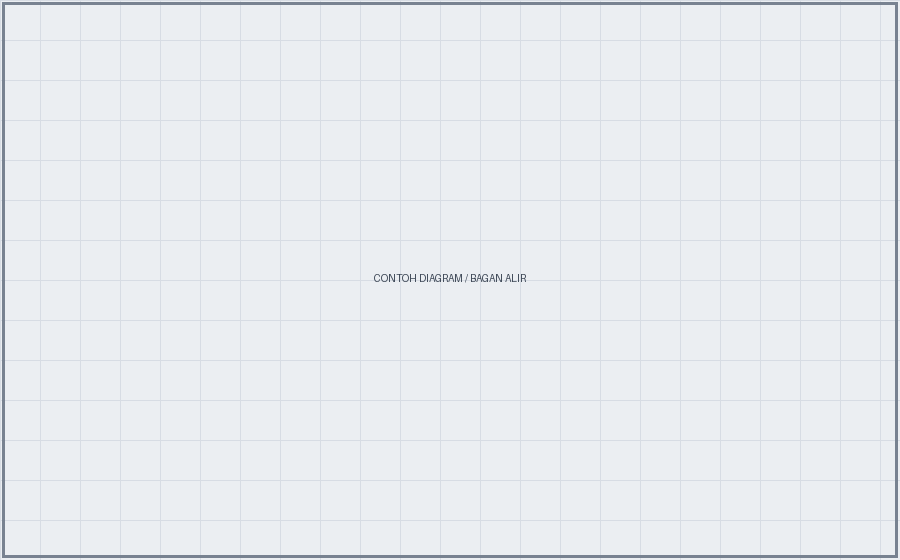
\includegraphics[width=0.6\linewidth]{contoh-diagram}
    \caption{Contoh gambar tunggal}
    \label{fig:g-tunggal}
\end{figure}

\subsection{Gambar dengan keterangan sumber}
Gunakan perintah \texttt{\textbackslash sumber} bila gambar dikutip dari
sumber lain.

\begin{figure}[H]
    \centering
    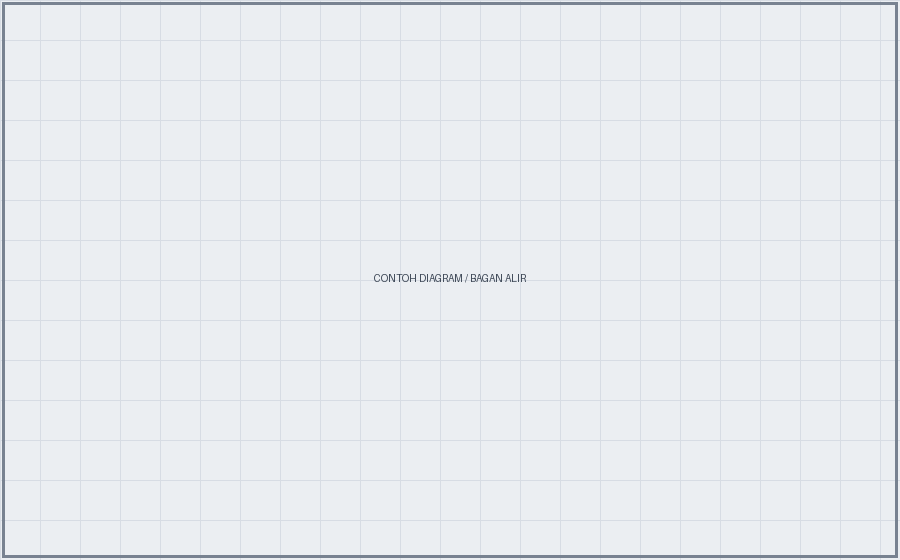
\includegraphics[width=0.55\linewidth]{contoh-diagram}
    \caption{Contoh gambar yang dikutip dari sumber lain}
    \label{fig:g-sumber}
\end{figure}
\sumber{\citet{barnes2002}}

\subsection{Dua gambar berdampingan}
Gunakan \texttt{subcaption} agar tiap bagian memperoleh label (a) dan (b) yang
dapat dirujuk terpisah, misalnya \cref{fig:g-kiri} dan \cref{fig:g-kanan}.

\begin{figure}[H]
    \centering
    \begin{subfigure}[t]{0.47\linewidth}
        \centering
        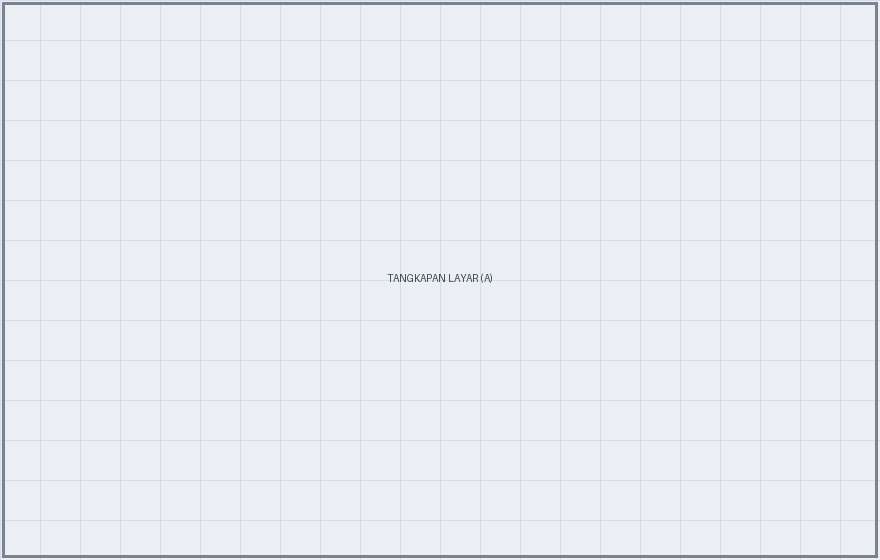
\includegraphics[width=\linewidth]{contoh-tangkapan-a}
        \caption{Tampilan sebelum perbaikan}
        \label{fig:g-kiri}
    \end{subfigure}
    \hfill
    \begin{subfigure}[t]{0.47\linewidth}
        \centering
        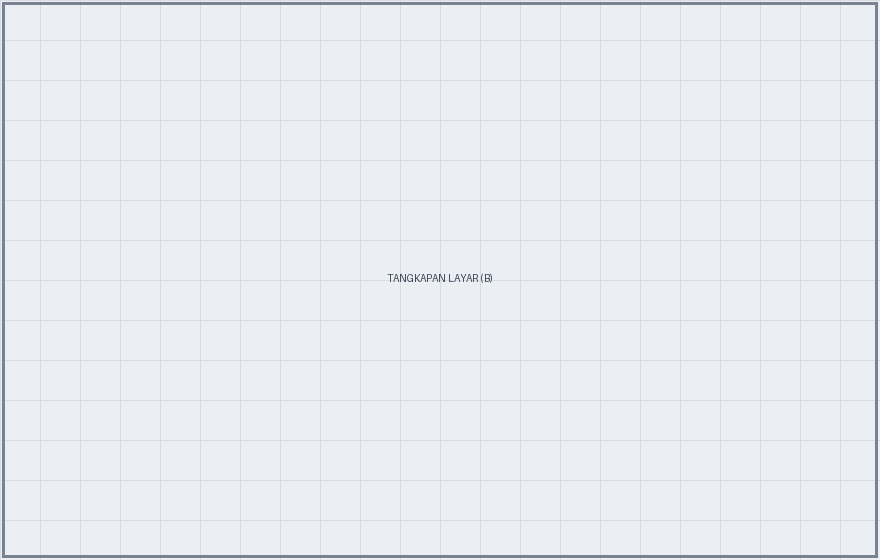
\includegraphics[width=\linewidth]{contoh-tangkapan-b}
        \caption{Tampilan sesudah perbaikan}
        \label{fig:g-kanan}
    \end{subfigure}
    \caption{Perbandingan tampilan antarmuka}
    \label{fig:g-berdampingan}
\end{figure}

\subsection{Gambar tinggi satu halaman}
Untuk gambar yang tinggi, seperti diagram alir panjang, gunakan
\texttt{height} agar tidak meluber ke halaman berikutnya.

\begin{figure}[H]
    \centering
    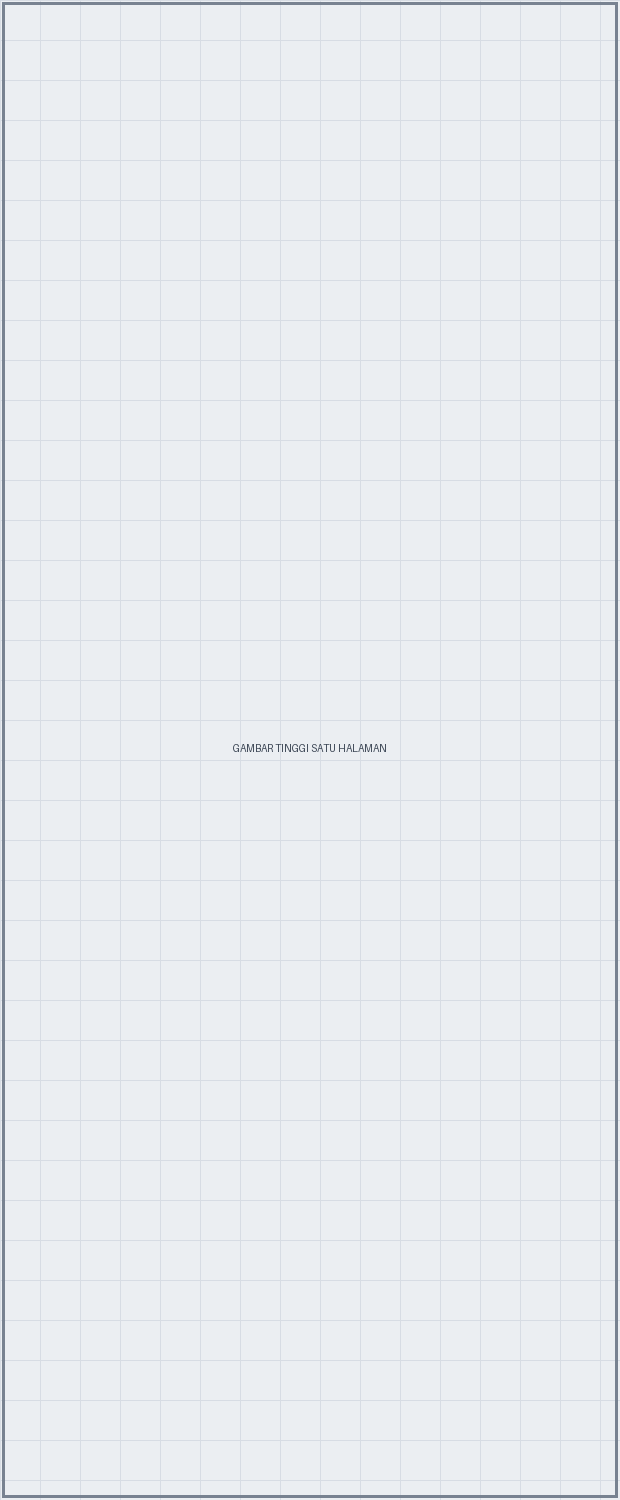
\includegraphics[height=0.78\textheight,keepaspectratio]{contoh-tinggi}
    \caption{Contoh gambar tinggi satu halaman}
    \label{fig:g-tinggi}
\end{figure}

\subsection{Gambar lanskap}

\begin{landscape}
\begin{figure}[H]
    \centering
    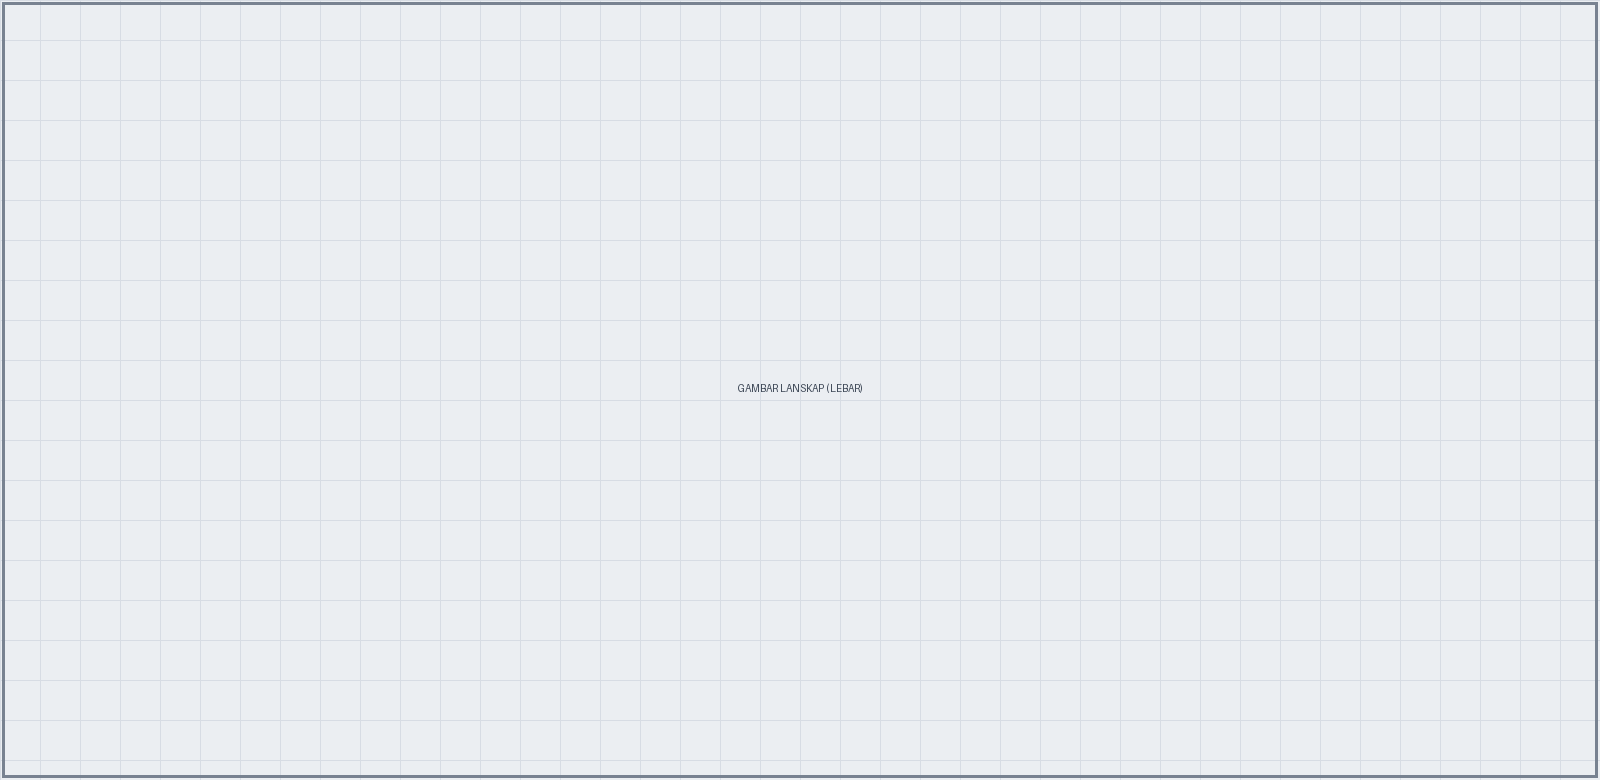
\includegraphics[width=0.92\linewidth]{contoh-lanskap}
    \caption{Contoh gambar pada halaman lanskap}
    \label{fig:g-lanskap}
\end{figure}
\end{landscape}

\subsection{Catatan penempatan gambar}
Parameter \texttt{[H]} memaksa gambar muncul tepat di posisi penulisannya.
Parameter \texttt{[htbp]} memberi LaTeX kebebasan menempatkan gambar pada
posisi terbaik, sehingga halaman tidak menyisakan ruang kosong. Gunakan
\texttt{[H]} bila urutan gambar penting, dan \texttt{[htbp]} bila
mengutamakan kerapian halaman.

% ==================================================================
\section{Persamaan}
% ==================================================================

Persamaan dalam baris teks ditulis seperti $\bar{x} = \sum x_i / n$, sedangkan
persamaan bernomor ditulis terpisah seperti \cref{eq:g-rerata}.

\begin{equation}
    \label{eq:g-rerata}
    \bar{x} = \frac{1}{n}\sum_{i=1}^{n} x_{i}
\end{equation}

Persamaan bertingkat ditulis dengan lingkungan \texttt{align}, dan setiap baris
memperoleh nomor tersendiri seperti \cref{eq:g-gap} dan \cref{eq:g-tki}.

\begin{align}
    \text{Gap}_i &= \bar{P}_i - \bar{I}_i \label{eq:g-gap} \\
    \text{TKI}_i &= \frac{\bar{P}_i}{\bar{I}_i} \times 100\% \label{eq:g-tki}
\end{align}

Beberapa bentuk yang sering dibutuhkan: pecahan $\frac{a}{b}$, akar
$\sqrt[3]{x}$, jumlah $\sum_{i=1}^{n}$, hasil kali $\prod_{i=1}^{n}$, integral
$\int_{0}^{1}$, huruf Yunani $\alpha, \beta, \sigma, \mu, \kappa$, serta matriks
berikut.

\begin{equation}
    \label{eq:g-matriks}
    \mathbf{D} =
    \begin{bmatrix}
        d_{11} & d_{12} & \cdots & d_{1n} \\
        d_{21} & d_{22} & \cdots & d_{2n} \\
        \vdots & \vdots & \ddots & \vdots \\
        d_{m1} & d_{m2} & \cdots & d_{mn}
    \end{bmatrix}
\end{equation}

% ==================================================================
\section{Kode Program}
% ==================================================================

\subsection{Kode ditulis langsung}
Kode dapat ditulis langsung di dalam naskah dan dirujuk seperti
\cref{lst:g-python}.

\begin{lstlisting}[language=Python, caption={Contoh kode Python}, label=lst:g-python]
def hitung_rerata(nilai):
    """Menghitung rata-rata dari sebuah senarai angka."""
    if not nilai:
        return 0
    return sum(nilai) / len(nilai)
\end{lstlisting}

\begin{lstlisting}[language=SQL, caption={Contoh kueri SQL}, label=lst:g-sql]
SELECT d.nama       AS dimensi,
       AVG(j.kinerja)     AS rerata_kinerja,
       AVG(j.kepentingan) AS rerata_penting
FROM   jawaban j
JOIN   butir b   ON b.id = j.butir_id
JOIN   dimensi d ON d.id = b.dimensi_id
GROUP  BY d.nama
ORDER  BY rerata_kinerja ASC;
\end{lstlisting}

\begin{lstlisting}[language=Java, caption={Contoh kode Java}, label=lst:g-java]
public class Responden {
    private final String kode;
    private final int[] jawaban;

    public Responden(String kode, int[] jawaban) {
        this.kode = kode;
        this.jawaban = jawaban;
    }

    public double rerata() {
        return Arrays.stream(jawaban)
                     .average()
                     .orElse(0.0);
    }
}
\end{lstlisting}

\begin{lstlisting}[language=PHP, caption={Contoh kode PHP}, label=lst:g-php]
<?php
function hitungGap(array $kin, array $pen): array {
    $gap = [];
    foreach ($kin as $b => $nilai) {
        $gap[$b] = round($nilai - $pen[$b], 2);
    }
    return $gap;
}
\end{lstlisting}

\subsection{Kode dibaca dari berkas}
Cara ini lebih dianjurkan untuk lampiran kode karena isinya selalu sinkron
dengan berkas sumber, dapat dicari, dan tidak membengkakkan ukuran berkas
seperti halnya tangkapan layar. Lihat \cref{lst:g-berkas}.

\lstinputlisting[language=Python, caption={Kode yang dibaca langsung dari berkas \texttt{kode/hitung-sus.py}}, label=lst:g-berkas]{kode/hitung-sus.py}

Sebagian baris saja juga dapat ditampilkan dengan parameter
\texttt{firstline} dan \texttt{lastline}.

\lstinputlisting[language=Python, firstline=7, lastline=18, caption={Cuplikan baris 7--18 dari berkas yang sama}, label=lst:g-cuplikan]{kode/hitung-sus.py}

\subsection{Pseudocode}
Untuk menuliskan algoritma, gunakan \texttt{algorithm2e}. Bentuk ini lebih
disukai penguji daripada kode nyata karena tidak terikat bahasa pemrograman
tertentu. Lihat \cref{alg:g-ipa}.

\begin{algorithm}[H]
\caption{Pemetaan kuadran \textit{Importance-Performance Analysis}}
\label{alg:g-ipa}
\KwMasukan{Senarai butir $B$, skor kepentingan $I$, skor kinerja $P$}
\KwKeluaran{Kuadran setiap butir}
$\bar{I} \leftarrow$ rata-rata seluruh nilai $I$\;
$\bar{P} \leftarrow$ rata-rata seluruh nilai $P$\;
\ForEach{butir $b \in B$}{
    \uIf{$I_b \geq \bar{I}$ \textbf{dan} $P_b < \bar{P}$}{
        $K_b \leftarrow$ ``Prioritas utama''\;
    }
    \uElseIf{$I_b \geq \bar{I}$}{
        $K_b \leftarrow$ ``Pertahankan prestasi''\;
    }
    \uElseIf{$P_b < \bar{P}$}{
        $K_b \leftarrow$ ``Prioritas rendah''\;
    }
    \Else{
        $K_b \leftarrow$ ``Berlebihan''\;
    }
}
\Return $K$\;
\end{algorithm}

% ==================================================================
\section{Sitasi dan Daftar Pustaka}
% ==================================================================

Template ini memakai gaya APA nama-tahun. Gaya diatur melalui perintah
\texttt{\textbackslash gayasitasi} pada berkas \texttt{a0-identitas.tex}.

\subsection{Bentuk sitasi}

\begin{daftarpoin}
    \item \texttt{\textbackslash citep\{kunci\}} menghasilkan sitasi dalam
          kurung: \citep{wijaya2022}. Dipakai bila rujukan bukan bagian dari
          kalimat.
    \item \texttt{\textbackslash citet\{kunci\}} menghasilkan sitasi naratif:
          \citet{wijaya2022}. Dipakai bila nama penulis menjadi subjek kalimat.
    \item Sitasi jamak ditulis dalam satu perintah:
          \citep{wijaya2022, pratama2023, sari2024}.
    \item Sitasi dengan halaman:
          \citep[hlm.~118]{barnes2002}.
    \item Sitasi dengan keterangan awalan:
          \citep[lihat][]{martilla1977}.
    \item Menyebut tahun saja: \citeyearpar{martilla1977}.
    \item Menyebut nama penulis saja: \citeauthor{barnes2002}.
\end{daftarpoin}

\subsection{Kutipan langsung}
Kutipan pendek ditulis menyatu dengan paragraf dan diapit tanda kutip.
Kutipan langsung yang panjang, yaitu lebih dari 40 kata, ditulis sebagai blok
tersendiri yang menjorok tanpa tanda kutip, seperti berikut.

\begin{quote}
    \noindent Tulis kutipan panjang Anda di sini. Blok kutipan ditulis menjorok
    ke dalam, tanpa tanda kutip, dan tetap diakhiri sitasi yang memuat nomor
    halaman sumbernya. Kutipan langsung sebaiknya digunakan seperlunya saja;
    utamakan parafrasa dengan bahasa Anda sendiri agar naskah tidak menjadi
    rangkaian kutipan. \citep[hlm.~120]{barnes2002}
\end{quote}

\subsection{Tipe entri pada berkas .bib}
Berkas \texttt{a7-pustaka.bib} memuat katalog seluruh tipe entri yang lazim
dipakai, yaitu \texttt{@article} untuk artikel jurnal, \texttt{@book} untuk
buku, \texttt{@incollection} untuk bab dalam bunga rampai,
\texttt{@inproceedings} untuk prosiding, \texttt{@mastersthesis} untuk skripsi
atau tesis, \texttt{@techreport} untuk laporan lembaga, \texttt{@manual} untuk
standar dan dokumentasi, serta \texttt{@misc} untuk sumber daring. Salin tipe
yang dibutuhkan lalu isi dengan data sebenarnya.

% Perintah \nocite berikut memaksa seluruh tipe entri ikut tampil pada
% Daftar Pustaka meskipun tidak disitasi di dalam teks, sehingga Anda
% dapat melihat bentuk tampilannya. Entri ini akan hilang sendiri
% begitu galeri dimatikan.
\nocite{contoh-buku, contoh-babbuku, contoh-prosiding, contoh-skripsi,
        contoh-laporan, contoh-standar, contoh-web}

Bentuk tampilan masing-masing tipe dapat Anda lihat langsung pada Daftar
Pustaka naskah ini.

% ==================================================================
\section{Rujukan Silang}
% ==================================================================

Seluruh rujukan silang sebaiknya memakai \texttt{\textbackslash cref} agar kata
``Gambar'', ``Tabel'', atau ``Persamaan'' muncul otomatis dan penomorannya
selalu sinkron: \cref{fig:g-tunggal}, \cref{tab:g-biasa}, \cref{eq:g-rerata},
\cref{lst:g-python}, dan \cref{alg:g-ipa}.

Beberapa objek sekaligus dapat dirujuk dalam satu perintah dan LaTeX akan
menyusun kata sambungnya sendiri: \cref{tab:g-biasa,tab:g-booktabs,tab:g-gabung}.

Rujukan ke rumusan masalah juga tersedia. Perintah \texttt{\textbackslash
cref\{rq:kualitas\}} menghasilkan \cref{rq:kualitas}, sehingga penomoran RQ di
seluruh naskah menyesuaikan sendiri bila urutannya diubah.


\end{document}
